\chapter{Advertisement video understanding through the lens of temporal context}

In this chapter, we will explore the role of temporal context in macro-level content understanding of dynamic sources, i.e., videos. Specifically, we consider advertisement videos due to their unique narrative structures of multiple short-term temporal context changes that are linked by a longer narrative thread. In order to study the context-driven approaches, we introduce a new ads-specific benchmark called \textbf{\textit{MM-AU}} with salient narrative-driven tasks for macro-level understanding, i.e., topic categorization, tone transition, and social relevance. An overview of this work can be seen in Fig \ref{advertisement video understanding}.

\begin{figure}
    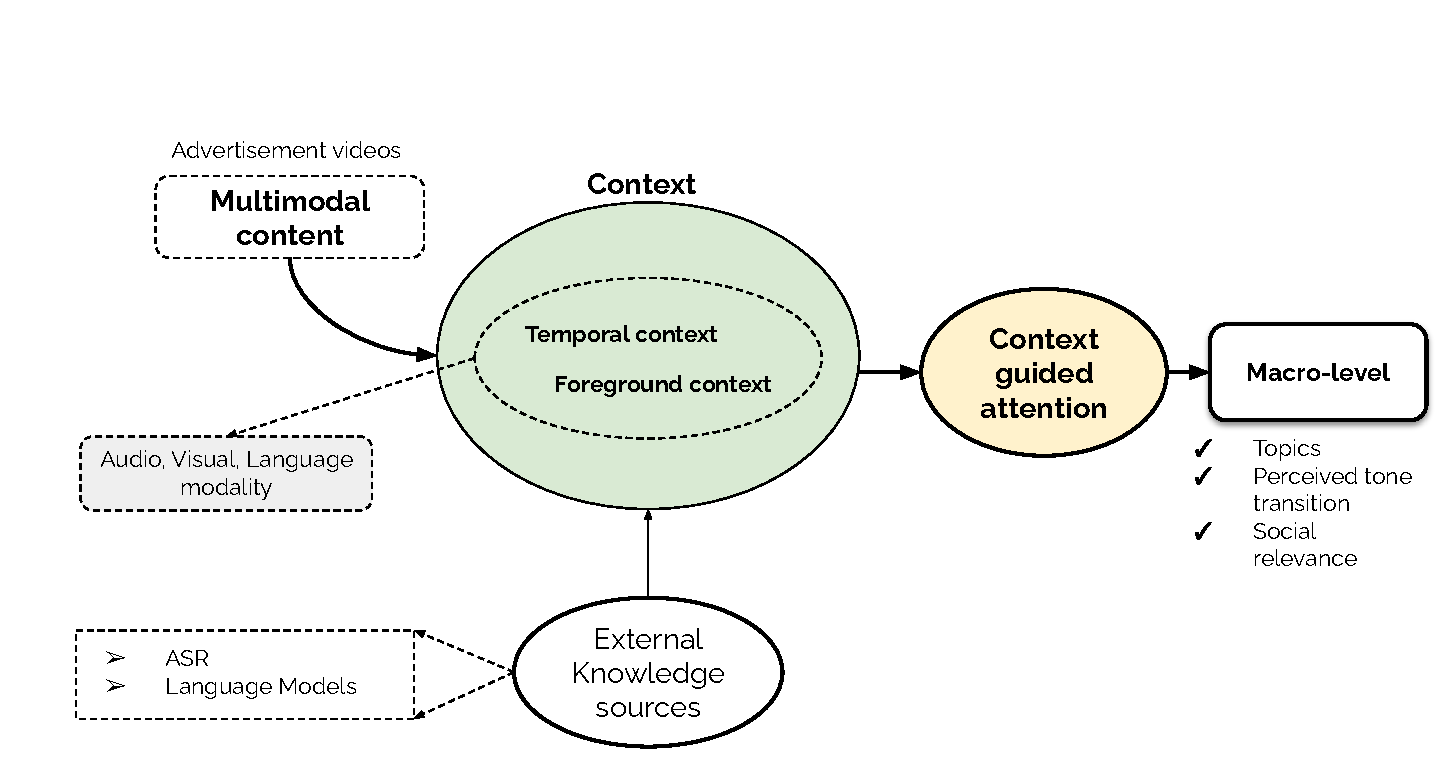
\includegraphics[width=\textwidth]{figures/advertisement_video_understanding.pdf}
    \caption{Overview of advertisement video understanding through the lens of temporal context}
    \label{advertisement video understanding}
\end{figure}

\section{Video Understanding}

Video Understanding aims to identify semantic elements from videos, including: \textit{environment}, \textit{objects}, \textit{actions}, \textit{events}, \textit{attributes}, \textit{concepts/themes} \cite{diba_large_2020}. Recognition of the semantic elements requires processing temporal context across different time scales, including short-term and long-term. As shown in Fig \ref{short term and long term context}, the short-term context in videos centers around visible human actions for a limited duration. However, long-term context consists of an integrated narrative spanning across multiple short-term context changes. In the case of movies, the long-term context can even span the entire duration of the movie. In this work, we primarily look at advertisement videos due to their unique narrative structure consisting of multiple short-term context changes along with long-term linkage within a limited time frame.

\begin{figure}[h!]
\centering
\subfloat[]{%
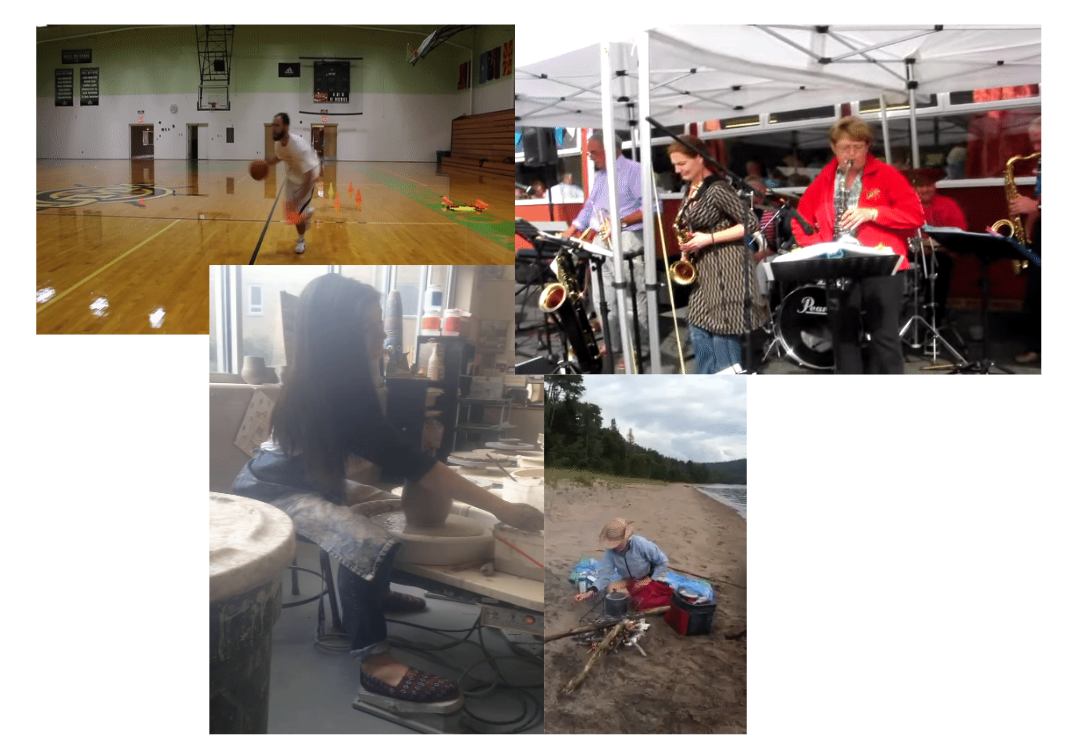
\includegraphics[width=0.5\textwidth]{figures/short_context_pictures.png}% 
\label{short context}
}
\subfloat[]{%
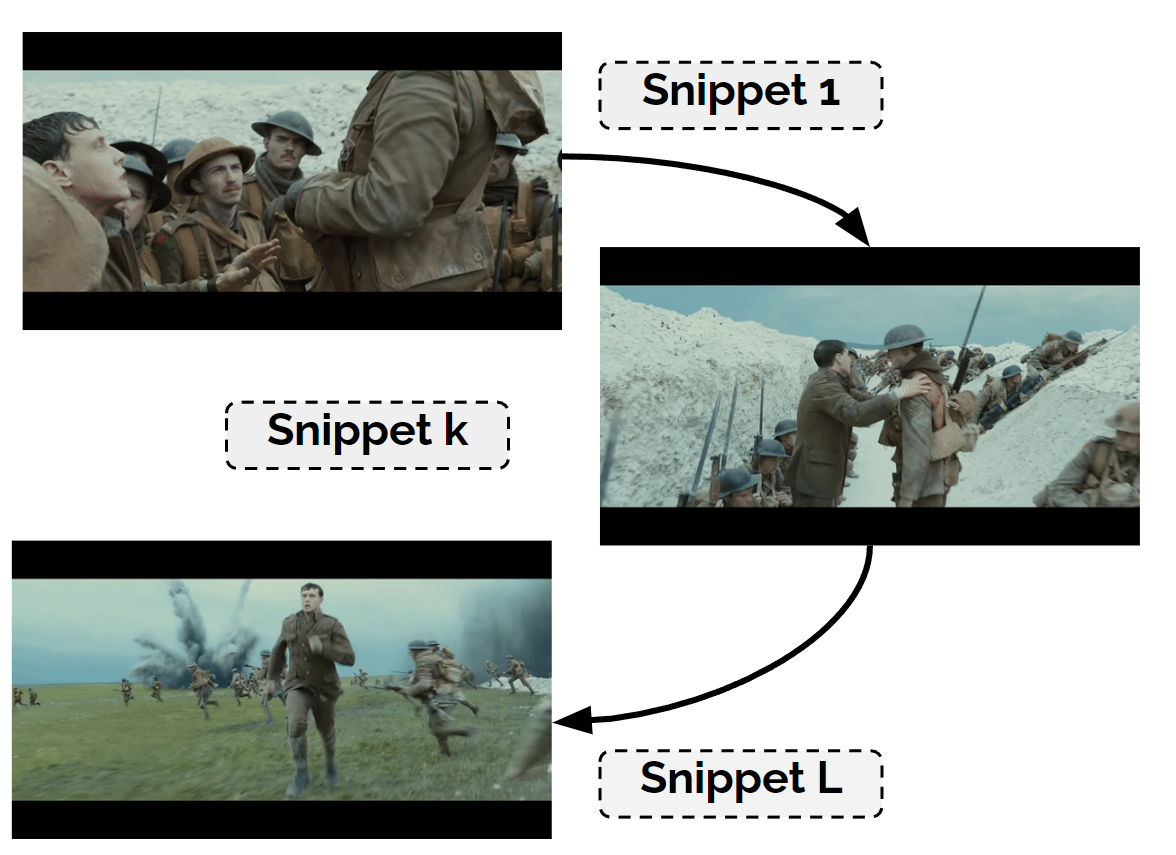
\includegraphics[width=0.5\textwidth]{figures/long_context_picture.png}%
\label{long context}
}
\caption{(a) Short-term context centered on human actions (b) Long-term context in movies useful for narrative understanding}
\label{short term and long term context}
\end{figure}

\section{Advertisements - Context transitions}

In terms of context transitions, advertisements lie between action-oriented short videos and feature-length movies. In Fig \ref{ads_structure_set}, we can see that multiple short-term context changes are happening due to the following sequence of activities/interactions:
\begin{itemize}
\item Police activity starting
\item Police chief gathering 
\item Police vehicles are getting destroyed
\item Children playing with toys 
\end{itemize}
From the sequence of events, it can be inferred that even though the short-term temporal information indicates negative situations, the overall theme revolves around toys for kids.
Thus, the temporal context information needs to be processed both locally and globally for a holistic understanding of ads at macro-level. 

\begin{figure}[h!]
\centering
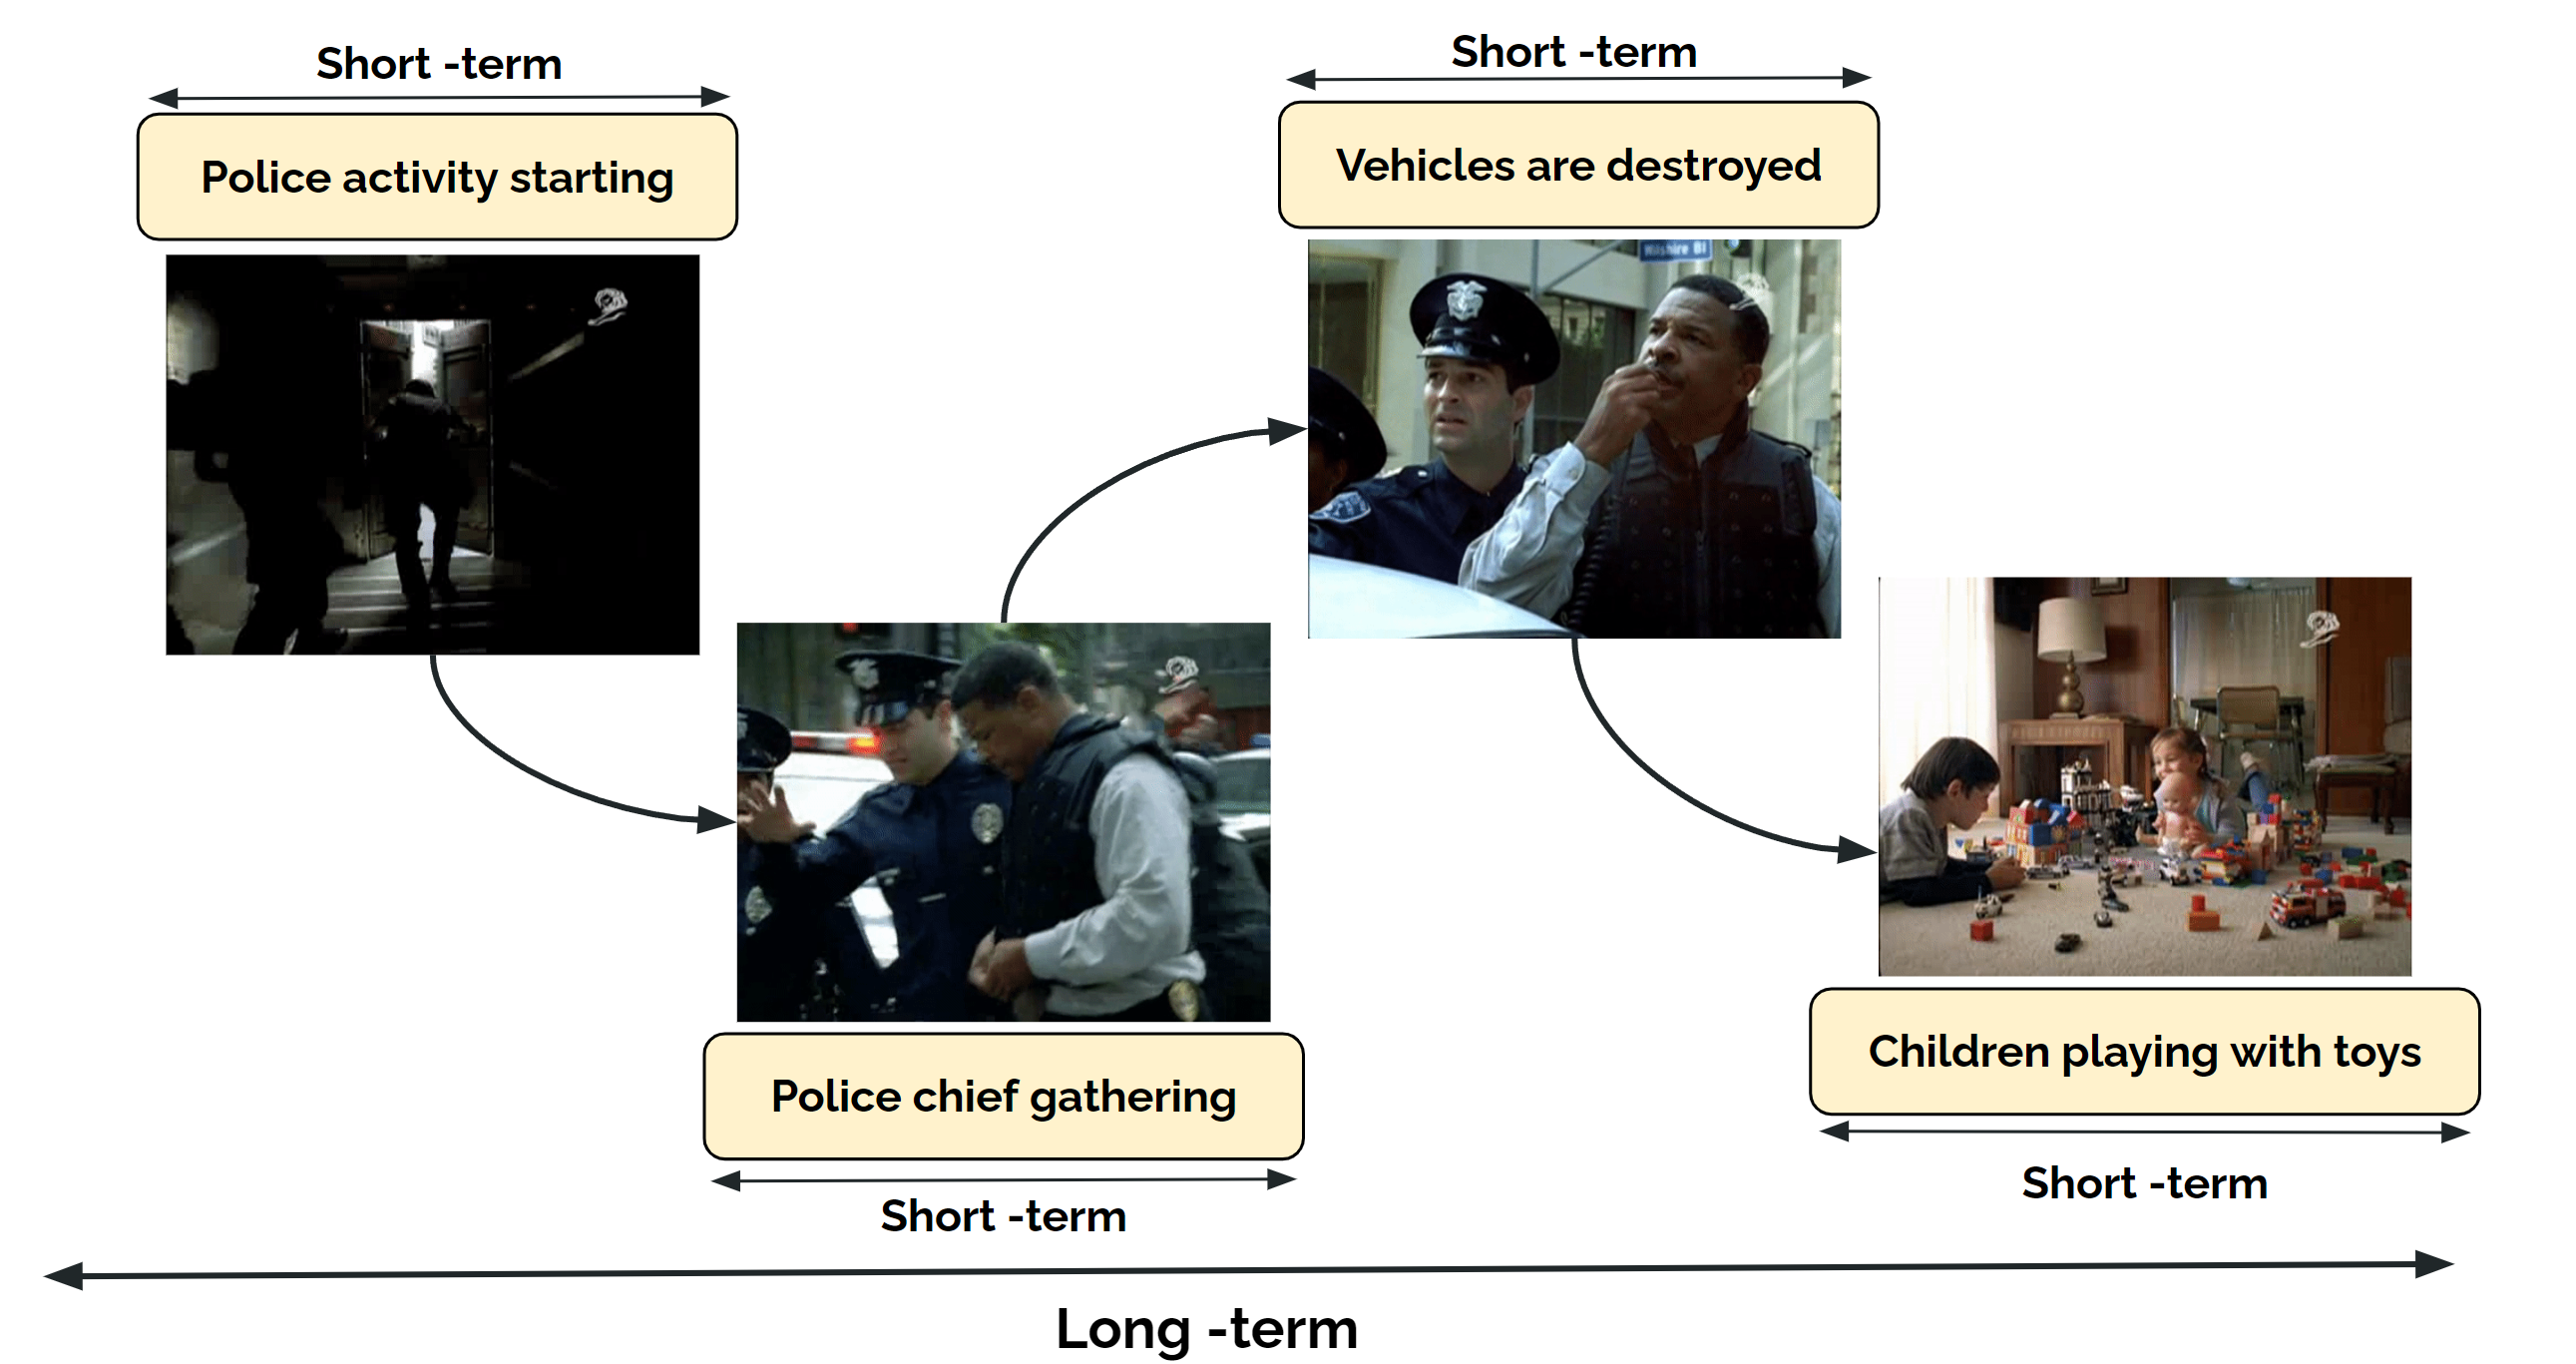
\includegraphics[width=\textwidth]{figures/ads_structure_figure.png}
\caption{Structure of advertisement video with multiple short-term context changes and overall long-term linkage}
\label{ads_structure_set}
\end{figure}

\section{Advertisements as medium}
As a primary media source for disseminating information, advertisements (ads for short) have been utilized to promote products or convey messages about extant social or political issues. The utility of advertisements as a media source has been amplified by the wide variety of platforms like radio, television, newspaper print, video streaming, and social networking sites, presenting significant influences, whether direct or indirect, to viewers from diverse backgrounds \cite{Pardun}. As shown in Fig \ref{ads_spending}, The rising importance of advertisements in the current socio-economic scenario is evident from the expected increase in media ad spending from 225.79 in 2020 to 322.11 billion dollars in 2024.

\begin{figure}[h!]
\centering
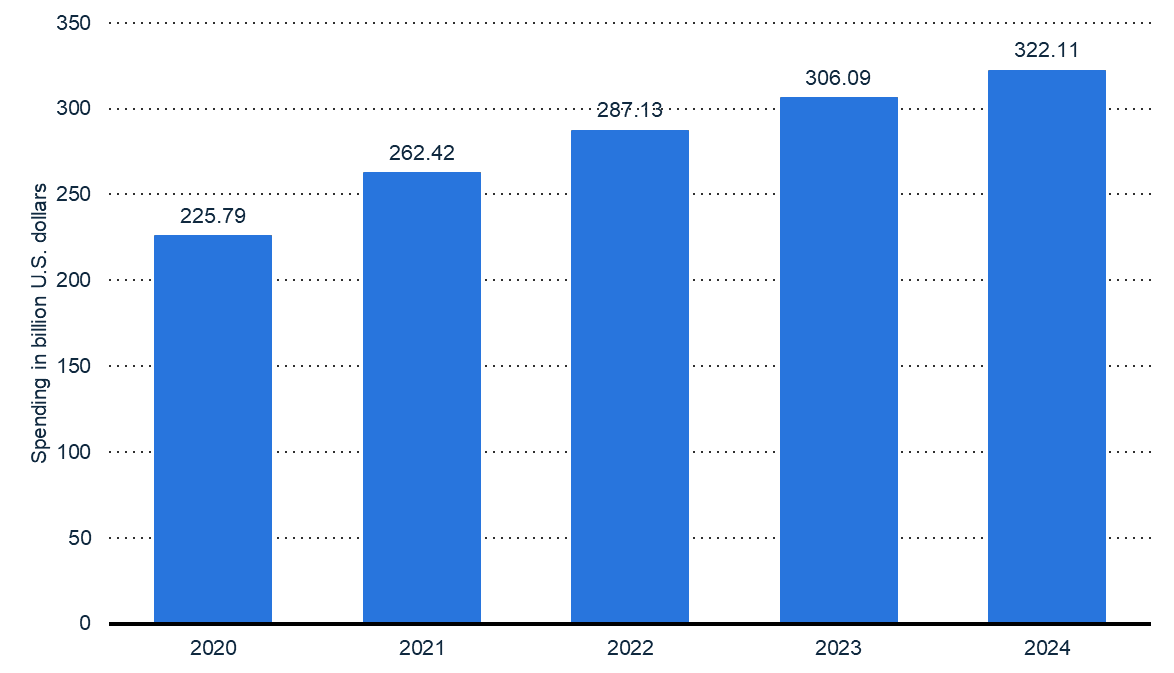
\includegraphics[width=0.8\textwidth]{figures/statistic_ads_spending.png}
\caption{Increase in demand for advertisements over last 4 years}
\label{ads_spending}
\end{figure}

\section{Advertisements - Narrative driven tasks and challenges}

Objectively understanding the rich content in ads and their impact on the viewer experience and behavior is hence of great interest. However, in enabling computational media understanding \cite{CMI}, advertisements present unique challenges in the form of condensed narrative structures \cite{Kim2017WhyNA}. Due to their relatively short duration when compared to feature-length movies, an advertisement video showcases a particular narrative structure in a tightly integrated sequence with different formats, including slice-of-life \cite{Mick1987TowardAS}, drama \cite{Leong1994UsingDT}, and transformational \cite{Puto1984InformationalAT}. Further, reasoning about the narrative structure requires a multi-scale understanding of the underlying topic and fine-grained elements, including the sequence of events (of characters and interactions) and related messages. As shown in Fig~\ref{introfig}, the key elements associated with the narrative structure of ads and related challenges are listed as follows:

\begin{figure}[h!]
\centering 
    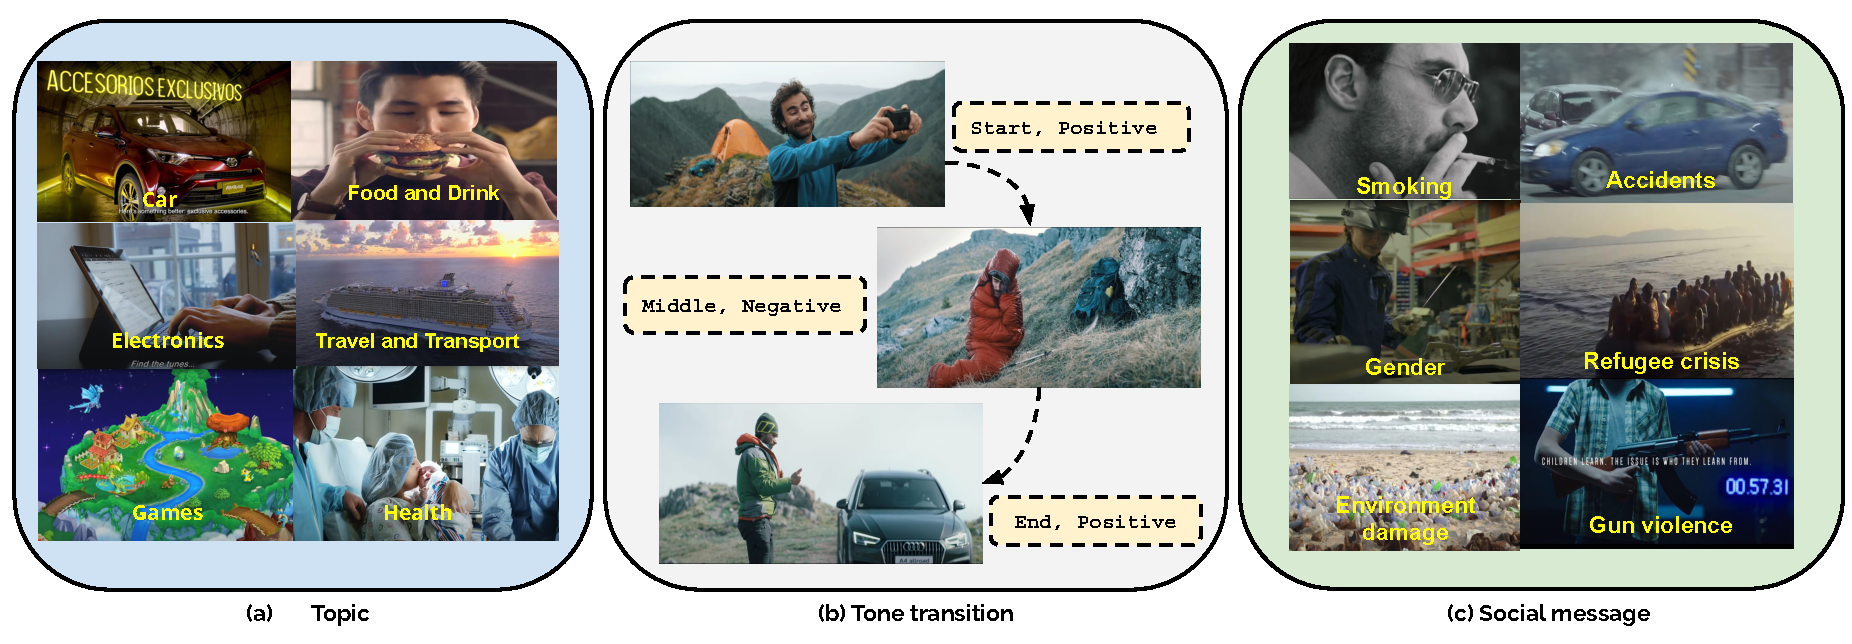
\includegraphics[width=0.8\textwidth]{figures/Task_outline_1_Topic_TT_SM.pdf}
  \caption{Schematic diagram showing illustrative examples of various tasks in the MM-AU (Multi-modal ads understanding) dataset. Multimodal understanding of ads along the lines of (a) Topic categorization (18 classes) (b) Tone transition (c) Social message detection i.e. Absence/Presence of social message}
  \label{introfig}
\end{figure}

\textbf{\underline{Topic}}: understanding enables personalized categorization and retrieval for customers along with key insights into the representation of genders \cite{google-diversity} and different demographic groups with respect to target classes like healthcare, retail, travel, etc. Topic categorization involves the handling of both inter and intra-topic diversity between the videos in terms of human-object interactions and a wide variety of items/products, as shown in Fig~\ref{introfig} (a). 

\textbf{\underline{Tone transition}}: Affective tone associated with an advertisement video refers to the perceived feeling by a viewer \cite{Veer2008HowTT}. Associating the appropriate tone with an ad enhances its persuasiveness, thus enabling the associated brand to expand its reach to a wide range of customers. While the positive tone centers around optimistic elements associated with hope and success \cite{Brooks2020ExploringAO}, portrayals of negative tone are tied to sad narratives involving fear and suffering. However, due to the narrative structure, the perceived affective tone exhibits transitions during the duration of an advertisement video, accompanied by changes in visuals and background music.  In Fig~\ref{introfig} (b), the video starts on a positive note with a happy person taking a picture, followed by a perceived negative tone in the middle due to the suffering of the person. The advertisement ends on a positive note, with the person being saved by an incoming vehicle.\\

\textbf{\underline{Social message}}: Advertisements act as a major source of information about pressing social issues for consumers. Brands conveying messages about various social issues, including but not limited to gender inequalities, racial discrimination, and environmental conservation, are viewed favorably by consumers across different age groups \cite{Brooks2020ExploringAO}. In terms of advertisement videos, social message portrayal is characterized by a huge diversity in depiction, as shown in Fig~\ref{introfig} (c) due to underlying categories like smoking, accidents, gun violence etc.

In this work, we introduce a multilingual multimodal benchmark called \textbf{\textit{MM-AU}} for the macro-level understanding of advertisement videos across the tasks of topic categorization, social message, and tone transition detection. Due to the inherent structure of the ads involving transitions in temporal context driven through multiple modalities, we propose context-guided attention mechanisms for the previously mentioned macro-level tasks. Our contributions can be listed as follows:
\begin{itemize}
    \item \textbf{\underline{Topic classification:}} We merge existing taxonomies for topic annotations from prior ads datasets and publicly available websites like {Ads of world}\footnote{https://www.adsoftheworld.com/} to obtain a condensed set of topic labels for the advertisement videos.
    \item \textbf{\underline{Tone Transition detection:}} We introduce a novel benchmark task of tone transition detection in advertisement videos by obtaining crowdsourced feedback from human annotators.
    \item \textbf{\underline{Social message detection:}} We provide weak human expert-based labels for detecting the presence/absence of social messages in advertisement videos.
    \item \textbf{\underline{Language-based reasoning:}} We explore zero-shot baselines for the three benchmark tasks through applications of large-language models on ad transcripts.
    \item \textbf{\underline{Context guided attention:}} We provide multiple context-guided attention baselines to benchmark the performance for the three macro-level tasks (topic classification, transition detection, and social message) and highlight future possibilities of explorations.
\end{itemize}
\section{Related work}
\textbf{Narrative understanding:} 
Narratives \cite{Fisher1987HumanCA} play an important role in enabling effective human communication and organizing the daily sequence of events. Advertisements centered on narratives \cite{Escalas1998ADVERTISINGNW} influence consumers by providing a concrete story arc centered around specific themes, protagonists, and their actions. Kim et al. \cite{Kim2017WhyNA} introduced an integrated theory of understanding narratives in advertisements based on key variables like emotic response, ad hedonic value, ad credibility, and perceived goal facilitation. Lien et al. \cite{Lien2013NarrativeAT} explored narrative ads from the lens of persuasion and the relationship with different advertisement mediums - verbal or visual. In the realm of computational narrative understanding, prior works have focused on language-based approaches for marking high-level structures in short stories \cite{Li2017AnnotatingHS}, most reportable events (MRE) in Reddit comment threads \cite{Ouyang2015ModelingRE} and primary processes in movie scripts, newspaper articles, etc \cite{Boyd2020TheNA}.\\
\textbf{Affect modeling in videos:}
Advertisement brands tend to invoke emotional reactions \cite{Holbrook1984TheRO} in viewers by influencing their actions i.e., purchasing a particular product. In the domain of television commercials, a combination of physiological, symbolic, and self-report measures was explored in \cite{Micu2010MeasurableEH} to determine the emotional responses of viewers. The role of facial expressions in decoding the preferences of viewers, including purchase intent, and smile responses, has been explored through large-scale studies in \cite{McDuff2014PredictingAL}, \cite{Teixeira2014WhyWA}. Apart from facial expressions, the role of CNN-based audio-visual and EEG descriptors from the viewers has been explored in a multi-task setup \cite{Shukla2017AffectRI,Shukla2017EvaluatingCV,Shukla2019RecognitionOA} for arousal and valence prediction in advertisement videos. Existing video-based affect datasets like DEAP \cite{Koelstra2012DEAPAD}, VideoEmotion \cite{Jiang2014PredictingEI} also focused on single arousal, valence, and dominance ratings as well as discrete emotion labels for music and user-generated videos, respectively.\\
In the domain of continuous affect modeling, datasets with frame-level annotations have been introduced across a wide variety of domains, including naturalistic and induced clips (HUMAINE \cite{DouglasCowie2007TheHD}), movies (COGNIMUSE \cite{Zlatintsi2017COGNIMUSEAM}, LIRIS-ACCEDE \cite{Baveye2015LIRISACCEDEAV}) and online videos (EEV \cite{Sun2020EEVDP}). Further extensions of continuous affect modeling based on independent and self-reports have been explored for daily emotional narratives in SENDv1 dataset \cite{Ong2019ModelingEI}. For advertisements, climax annotations (presence + rough timestamps) were provided by human annotators on a subset of the Video Ads dataset \cite{Hussain2017AutomaticUO} in \cite{Ye2018StoryUI} along with climax-driven modeling strategies to predict sentiment labels at the video level. 
In our proposed benchmark \textbf{\textit{MM-AU}}, based on the standard definition in \cite{Brooks2020ExploringAO}, we ask human annotators to denote the perceived tone in the advertisement video across segments approximately marking the start, middle, and end. The perceived tone transition enables tracking of the narrative dynamics in advertisement videos by considering the interactions between various contextual streams through different modalities, i.e. audio, visual, and narrations/spoken interactions (through transcripts).\\
\textbf{Advertisement benchmarks:} 
\begin{table*}[h!]
\centering
\resizebox{\textwidth}{!}{
\begin{tabular}{|c|c|c|c|c|c|c|c|c|}
\hline
\textbf{Dataset}       & \textbf{Annotation type} & \textbf{Duration} & \textbf{\#Samples} & \textbf{\#Shot} & \textbf{\#Class}                     & \textbf{Modalities}      & \textbf{Languages}                   & \textbf{Tasks}                      \\ \hline
Video Ads Dataset (I)  & H                        & NA                & 64832              & NA              & 38 (T), 30 (S), AR (OE), H(2), Ex(2) & Images                   & English                              & Image level classification          \\ \hline
Video Ads Dataset (V)  & H                        & 144.87            & 3477               & NA              & 38 (T), 30 (S), AR (OE), H(2), Ex(2) & Video                    & English                              & Video level classification          \\ \hline
Tencent-AVS            & H                        & 142.1h            & 12k                & 121.1k          & 25 (Pr), 34 (St), 23 (Pl)            & Video/Audio/ASR/OCR              & Chinese and English                  & Scene level classification          \\ \hline
Ads-persuasion dataset & H + AL                   & NA                & 3000               & NA              & 21 (PS)                              & Images                   & English                              & Image level classification          \\ \hline
E-MMAD                 & SG descriptions          & 1021.6 h          & 120984             & NA              & 4863 (PC)                            & Video                    & Chinese and English                  & Video level captioning              \\ \hline
\textbf{MM-AU}         & \textbf{H + SA}          & \textbf{147.8h}   & \textbf{8399}      & \textbf{216.4k} & \textbf{18 (T), 3 (Tone), 2 (SM)}    & \textbf{Video/Audio/ASR} & \textbf{Multilingual (65 languages)} & \textbf{Video level classification} \\ \hline
\end{tabular}
}
\vspace{5mm}
\caption{Comparison of \textbf{\textit{MM-AU}} with other available advertisement benchmarks across different modalities.  \underline{Annotation type:} \textbf{H}: Human annotation, \textbf{AL}: Active Learning, \textbf{SA}: Semi-automatic, \textbf{SG}: Store generated. \underline{Duration:} \textbf{NA}: Not applicable for images; Mentioned in hours(h). \underline{\#Samples:} Number of video clips or images. \underline{\#Shot:} \textbf{NA}: Not applicable for images; Number of shots detected from all the video samples. \underline{\#Class:} \textbf{T:} Topic, \textbf{S:} Sentiment, \textbf{OE:} Open-Ended, \textbf{H:} Humor, \textbf{Ex:} Exciting, \textbf{Pr:} Presentation, \textbf{St:} Style, \textbf{Pl:} Place, \textbf{PS:} Persuasion strategy, \textbf{PC:} Product categories, \textbf{SM:} Social messages}
\label{Overview_ads}
\end{table*}

While there has been progress in terms of movie understanding due to the introduction of large-scale multimodal benchmark datasets like Condensed Movies \cite{bain2020condensed}, MovieNet \cite{huang2020movienet}, MAD \cite{Soldan_2022_CVPR}, Movie-cuts \cite{Pardo2021MovieCutsAN}, MovieCLIP \cite{Bose_2023_WACV} and SAM-S \cite{Hebbar2023ADF}, only few benchmarks have focused on large-scale understanding of advertisements across broad and fine-grained content. Hussain et al. \cite{Hussain2017AutomaticUO} introduced the benchmark Video-Ads dataset to facilitate understanding of images and videos along the lines of broad topics, induced sentiments, and action/intent reasoning. The images in the Video-Ads dataset were utilized in \cite{Singla2022PersuasionSI} for computational modeling of persuasion across 21 categories in marketing domain. Regarding large-scale ads understanding, Tencent-AVS dataset \cite{Jiang2022TencentAA} was proposed to enable multi-modal scene level categorization into semantic classes like presentation, places and styles. While the previously mentioned datasets focused on classification tasks, E-MMAD \cite{Zhang2022AttractMT} introduced the task of informative caption generation from advertisements across 120k e-commerce videos.
\\
\textbf{\textit{MM-AU}}, our curated multilingual dataset utilizes publicly available videos from Ads of the World along with a subset from Video-Ads dataset and an in-house video catalog from Cannes Lion archive \cite{cannes-lions}. We provide 18 broad topic categories by combining existing taxonomies (Cannes Lion, Ads of World, and Video-Ads dataset). Further, we rely on human expert annotators to label transitions in perceived tone along with the absence/presence of social messages in 8.4K advertisement videos. A comparative overview of \textbf{\textit{MM-AU}} and other advertisement datasets is shown in Table \ref{Overview}.\\
\textbf{Semantic video understanding:}
Existing large-scale video datasets including Kinetics\cite{Carreira2017QuoVA}, Moments-in-time \cite{Monfort2018MomentsIT}, ActivityNet \cite{Heilbron2015ActivityNetAL}, AVA \cite{Gu2017AVAAV} have focused mainly on classifying entity driven actions from in-the-wild short videos. Higher-level semantic labels beyond actions like topics, concepts, events, and video types were exploited for large-scale video-level categorization in datasets like Youtube-8M \cite{AbuElHaija2016YouTube8MAL}, Holistic-visual understanding (HVU) \cite{diba2020large} and 3MASSIV \cite{Gupta20223MASSIVMM}. Our proposed benchmark \textbf{\textit{MM-AU}} explores the domain of semantic video understanding in ads by considering broad categories like topic, presence/absence of social message, and fine-grained affective labels of perceived tone transition.\\
\textbf{Multimodal representation learning:} Multimodal representation learning \cite{Liang2022FoundationsAR} centers around the fusion of information from different modalities at multiple scales, including early, late, and mid-fusion. Prior works related to ads have utilized multimodal-LSTMs \cite{Vedula2017MultimodalCA}, segment-level autoencoders \cite{SomandepJointenc} or joint cross-modal embedding \cite{Ye2019InterpretingTR} approaches for learning multimodal representations for a variety of tasks. With the advent of transformer \cite{transformers} based multimodal models like PerceiverIO \cite{Jaegle2021PerceiverIA}, attention bottlenecks\cite{nagrani2021attention}, and VATT \cite{Akbari2021VATTTF}, information fusion at the input token space, followed by joint encoders, have become more prevalent. A multi-task attention-based approach was explored in \cite{LookReadFeel} for jointly predicting topic and sentiment labels associated with advertisement images. A NextVLAD \cite{Lin2018NeXtVLADAE} based approach \cite{Weng2021AMF} combined with global-local attention was utilized for predicting scene-specific labels in the Tencent \cite{Jiang2022TencentAA} ads benchmark dataset.
\section{MM-AU benchmark}
\subsection{Data sources}
We consider multiple ads-specific sources for curating our proposed MM-AU dataset. As a primary source, we consider Ads-of-the-world (AOW)\footnote{https://www.adsoftheworld.com/} video hosting website since it contains a richly-curated catalog of ads in various formats like film, print, digital, and video spanning across multiple countries. As auxiliary sources, we consider additional videos from the Cannes Lion Film Festival archive and Video-Ads dataset \cite{Hussain2017AutomaticUO}. We filter the videos based on unique video ids associated with their public links to ensure no duplicates across three sources. The share of different sources in curating the combined list of 8399 advertisement videos is shown in Fig~\ref{ads_sources}
\begin{figure}[h!]
    \centering
    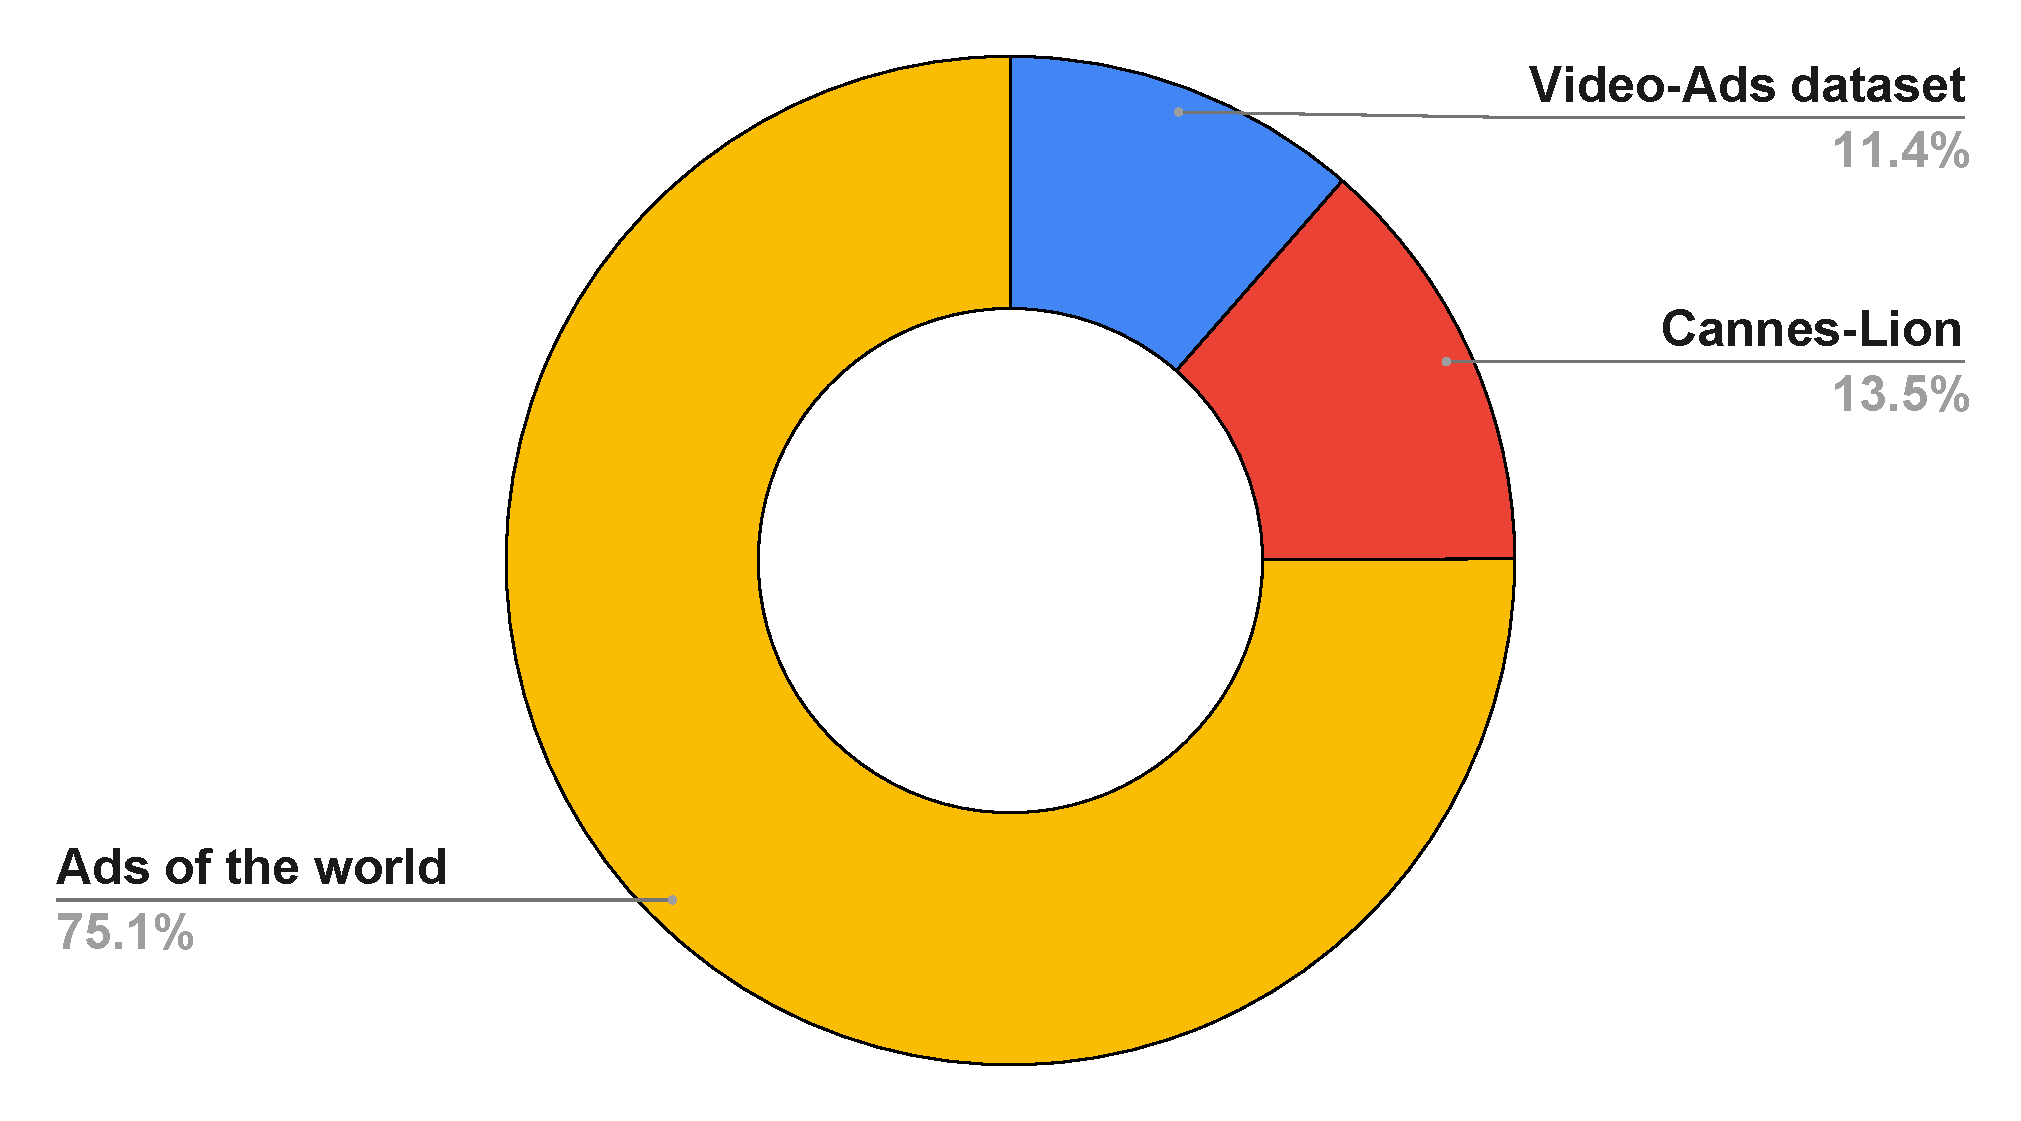
\includegraphics[width=0.8\textwidth]{figures/data_sources_distribution.pdf}
    \caption{Share of different ad sources in MM-AU dataset. Ads of the world (6304 videos), Cannes Lion (1135), Video-Ads dataset (960) }
    \label{ads_sources}
\end{figure}

\subsection{Human expert-driven annotations}
We employ a semi-automatic process for tagging the advertisement videos with broad topic categories. For the detection tasks of tone transition and social message, we use Amazon Mechanical Turk \footnote{https://www.mturk.com/} to obtain responses from a pool of 36 human annotators. 
For selecting a pool of workers with the requisite expertise, we hosted an initial pilot study where the workers are instructed to mark the tone transition labels and presence/absence of social message in the given set of videos. Further, in the final annotation phase, three annotators independently annotate each sample for the tone-transition and social message detection tasks. 
The annotation process details associated with the respective tasks are listed below:\\
\textbf{\underline{Tone transition:}} The annotators are instructed to mark the perceived tone labels associated with the start, middle, and ending segments of the advertisement videos. To reduce the burden associated with the task, no instructions are provided to mark the timestamps associated with the respective segments. 
\begin{figure*}[h!]
    \centering
    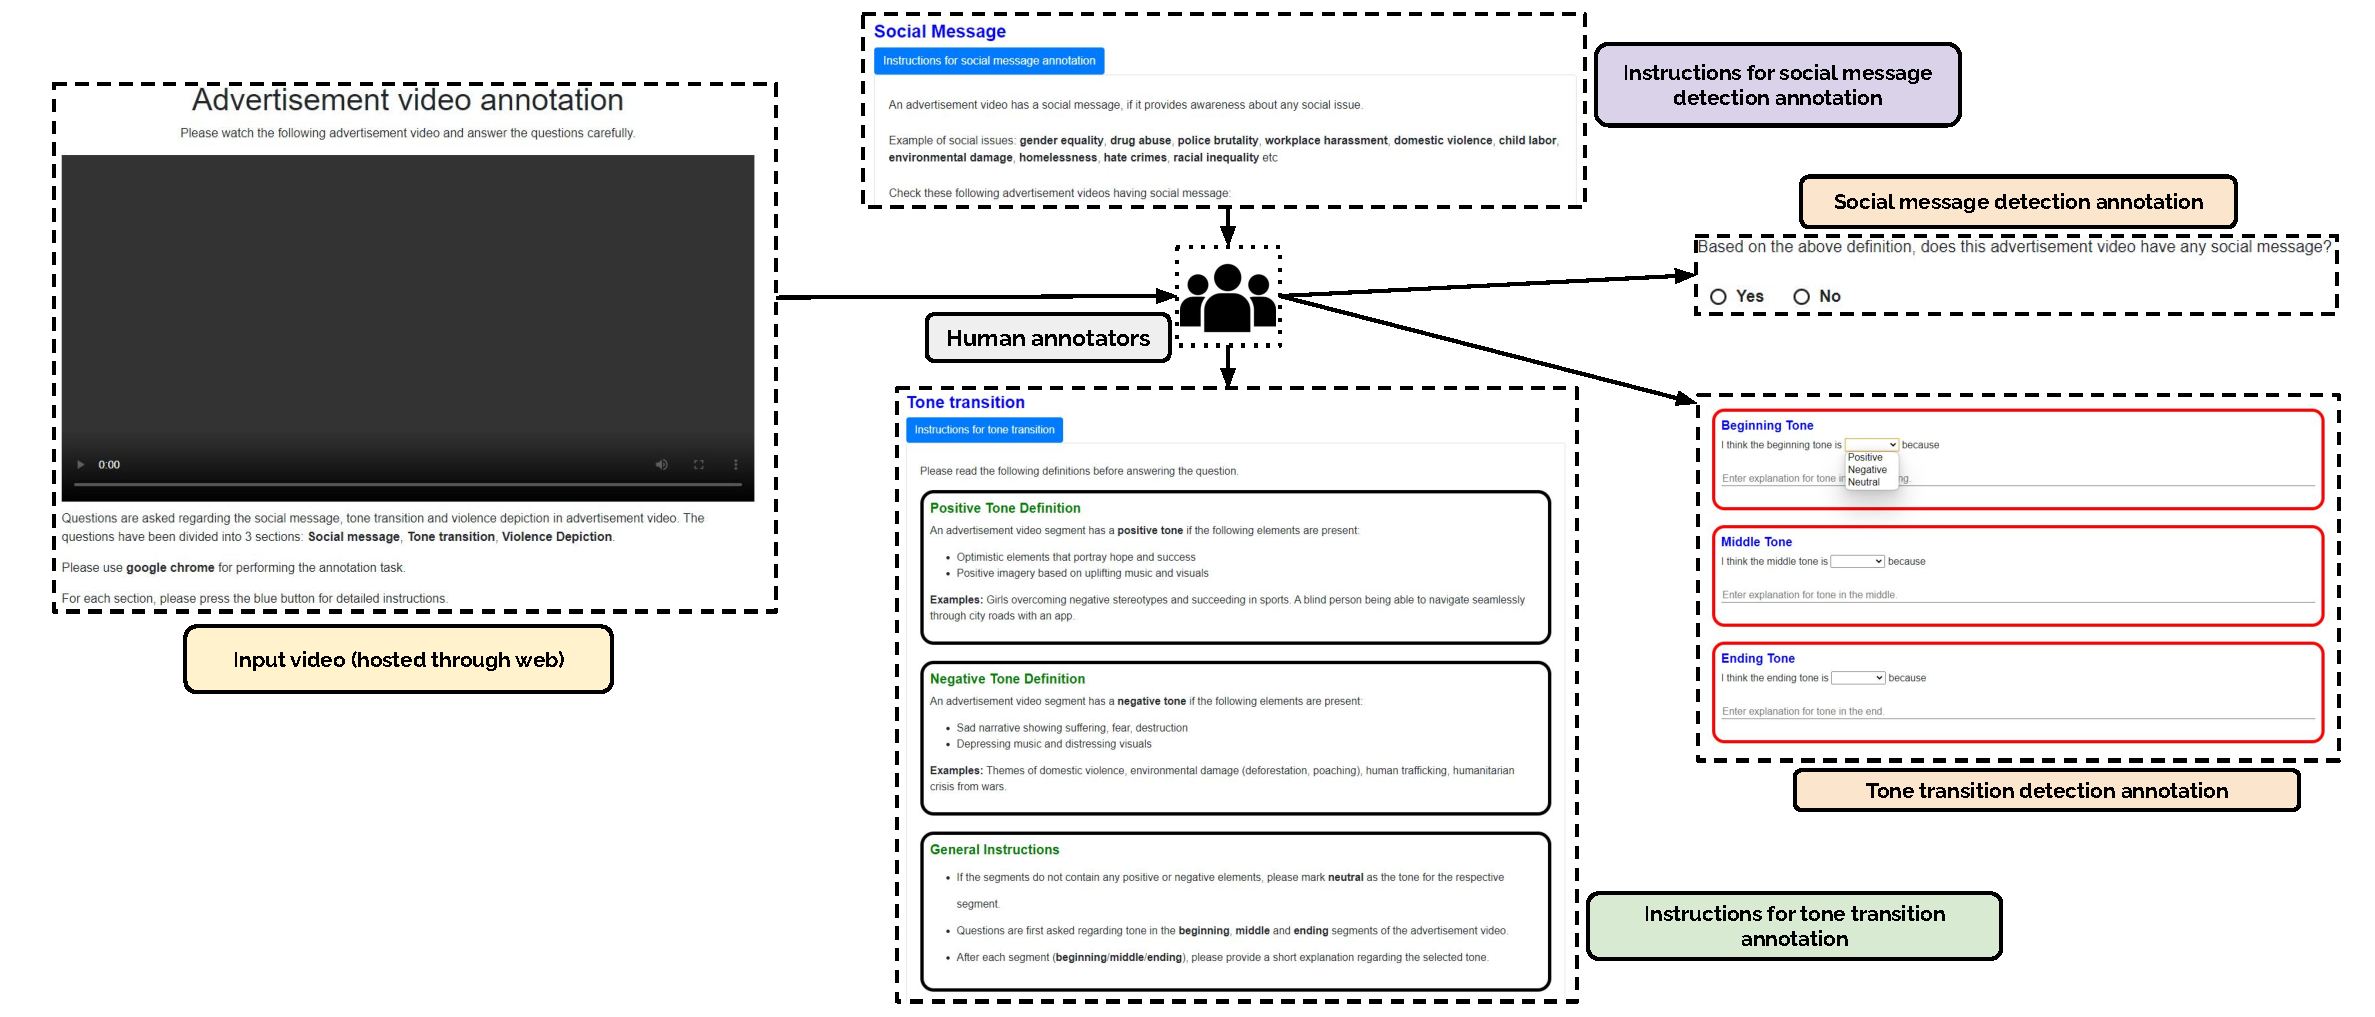
\includegraphics[width=\textwidth]{figures/Annotation_Flow_Part_2_updated.pdf}
    \caption{Outline of the annotation framework for tone transition and social message detection problem}
    \label{annot_framework}
\end{figure*}
Based on the tone definition considered in \cite{Brooks2020ExploringAO}, we provide the following descriptions to aid the annotation process:
\begin{itemize}
    \item \textbf{Positive tone:} An advertisement video segment has a positive tone if it contains: \textit{optimistic elements portraying hope and success} or \textit{positive imagery based on uplifting music and visuals}. Examples include girls overcoming negative stereotypes and succeeding in sports or a blind person being able to navigate easily through city roads by using an app.
    \item \textbf{Negative tone:} An advertisement video segment has a negative tone if it contains: \textit{sad narrative showing suffering, fear, destruction} or \textit{depressing music and distressing visuals}. Salient themes associated with negative tone include domestic violence, environmental damage, human trafficking, crisis from wars etc.
\end{itemize}
If a segment does not contain the above-mentioned characteristics, the annotators are instructed to mark the perceived tone as neutral. To determine the reasoning involved in marking the tone labels associated with the segments, the annotators are also asked to provide explanations regarding their choices. In Fig \ref{annot_framework}, we show the outline of the framework provided to the annotators for marking the tone associated with the start, middle, and end segments and the absence/presence of a social message. We provide a sample example to the annotators regarding tone transition and associated explanations, as shown in Fig \ref{tone_transition}. As seen in Fig \ref{tone_transition}, the beginning (start) segment has a perceived \textcolor{red}{\textbf{negative}} tone because police activity is being shown. The middle segment also shows a \textcolor{red}{\textbf{negative}} tone because vehicles are being destroyed, followed by a \textcolor{blue}{\textbf{positive}} tone at the ending portion because the kids are playing with toys.
\begin{figure}[h!]
    \centering
    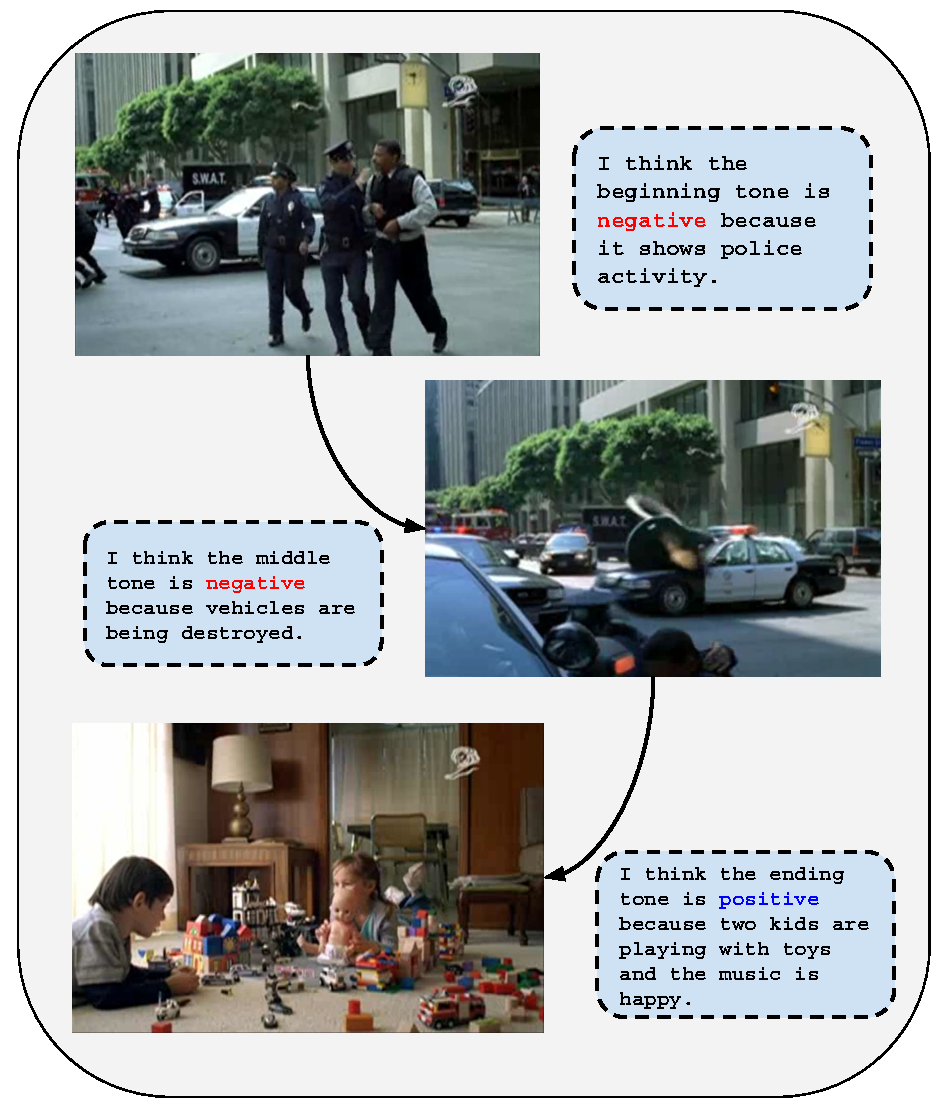
\includegraphics[width=0.5\columnwidth]{figures/Annotation_examples_tone_transition_new.pdf}
    \caption{Example provided to the annotators showing the tone transition and associated explanations}
    \label{tone_transition}
\end{figure}
\\
\textbf{\underline{Social message detection:}} For social message detection, the annotators are instructed to check for the absence/presence of social messages in the given video. Based on the social message framing in ads \cite{Brooks2020ExploringAO}, we provide the following definition to guide the annotation process:
\begin{itemize}
    \item An advertisement video has a social message if it provides awareness about any social issue. Examples include \textit{gender equality}, \textit{drug abuse}, \textit{police brutality}, \textit{workplace harassment}, \textit{domestic violence}, \textit{child labor}, \textit{homelessness}, \textit{hate crimes} etc.
\end{itemize}
To simplify the annotation process, we ask the annotators to mark Yes/No for indicating the presence/absence of social messages in the videos instead of marking the exact categories in the curated list of social issues \cite{ciment2006social}. The outline of the framework provided to annotators for marking the presence/absence of social messages is shown in Fig \ref{annot_framework}.
Further, annotators are also provided with example videos showing different forms of social messages. In Fig \ref{social_message} (a), frame transitions are shown from an example video urging everyone to vote since voters having bias can cast votes in their absence. In Fig  \ref{social_message} (b), sample frames in the sequence are shown from another example video highlighting the importance of equal opportunities for everyone in sports.
\begin{figure*}[h!]
\centering
    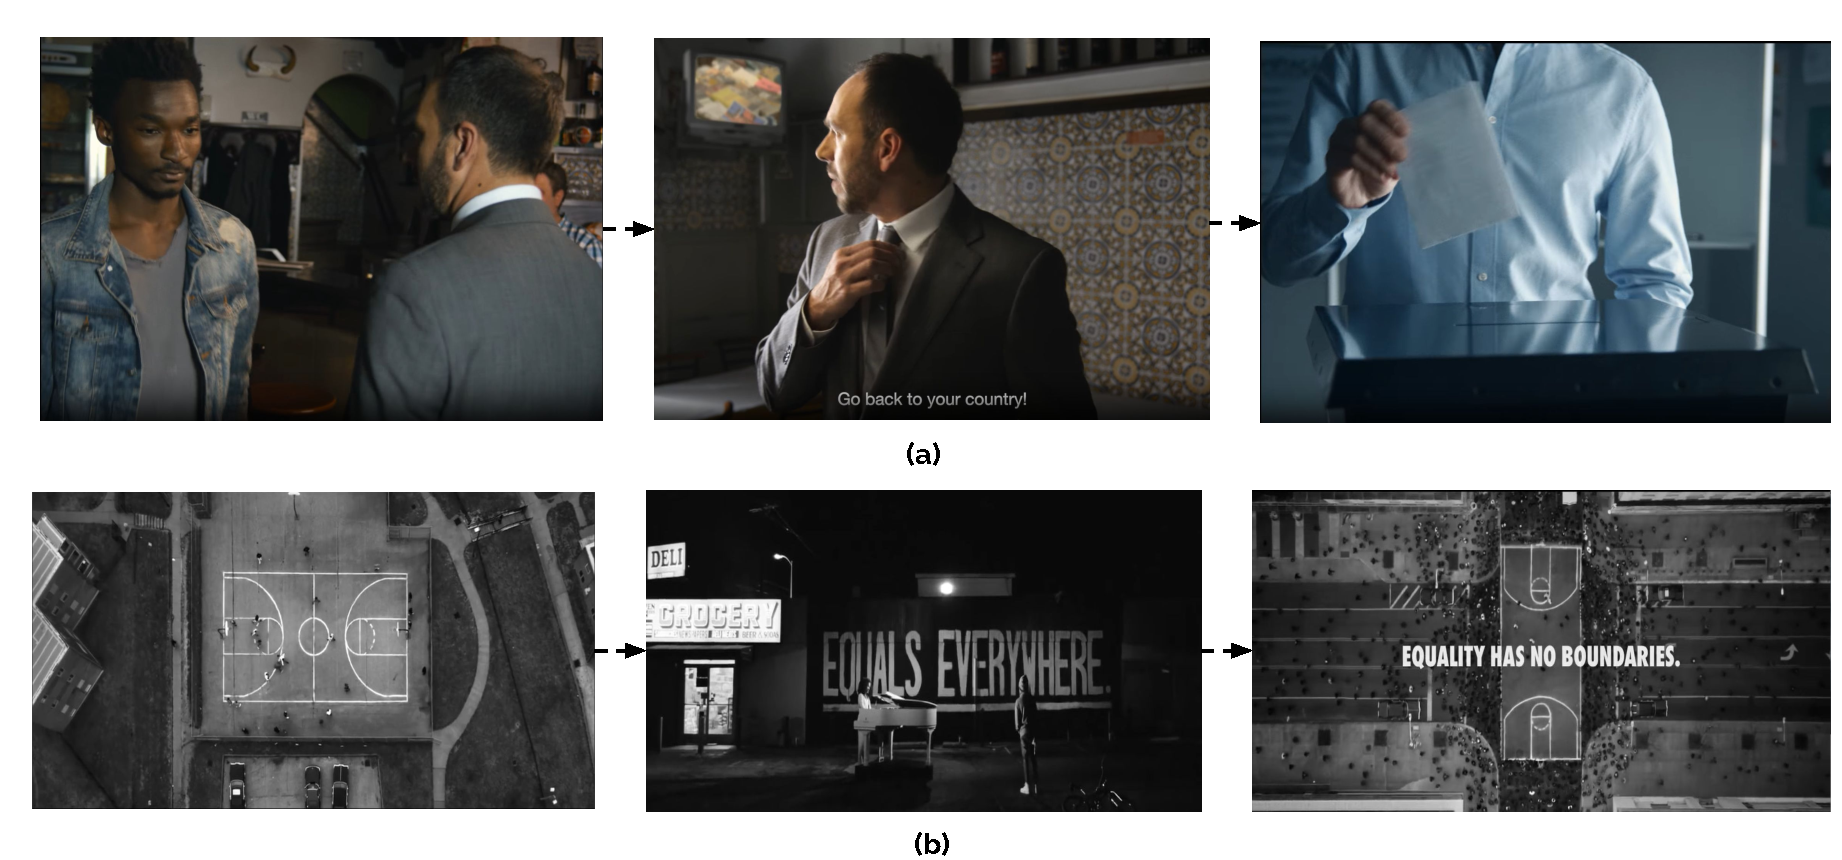
\includegraphics[width=0.8\textwidth]{figures/new_social_message_image.pdf}
    \caption{Example videos associated with absence/presence of social message provided to the annotators. (a) Frame transition associated with an example video urging people to vote (b) Frame transition associated with an example video emphasizing equal opportunities for everyone in sports.}
    \label{social_message}
\end{figure*}
\\
\textbf{\underline{Topic categorization:}}
We annotate topic categories using the existing taxonomies from Ads-of-the-world (AOW), Cannes Lions Film Festival \cite{cannes-lions}, and Video-Ads \cite{Hussain2017AutomaticUO} datasets. We denote the taxonomies associated with Cannes Lions Film Festival and Video-Ads datasets as Cannes-coding [\textcolor{purple}{\textbf{CC}}] and Video-Ads [\textcolor{blue}{\textbf{VA}}] coding schemes. 
We extract the available tags associated with 6304 videos in Ads-of-the-world [\textcolor{red}{\textbf{AOW}}] and retain the top 40 tags based on frequency. Then we manually merge the filtered topic tags from AOW with similar labels in Cannes-coding  [\textcolor{purple}{\textbf{CC}}] and Video-Ads [\textcolor{blue}{\textbf{VA}}] coding schemes. Some examples of merged labels from different sources are listed as follows with the final parent topic category:
\begin{itemize}
    \item \textbf{Publications media:} Media \& Publications  [\textcolor{purple}{\textbf{CC}}]; Media and arts [\textcolor{blue}{\textbf{VA}}]; TV Promos, Music, Media, Movies [\textcolor{red}{\textbf{AOW}}]
    \item \textbf{Games:} Games and toys [\textcolor{blue}{\textbf{VA}}]; Gaming [\textcolor{red}{\textbf{AOW}}]
    \item \textbf{Sports:} Sports equipment and activities [\textcolor{blue}{\textbf{VA}}]; Sports [\textcolor{red}{\textbf{AOW}}]
    \item \textbf{Clothing:} Clothing, Footwear \& Accessories [\textcolor{purple}{\textbf{CC}}]; Clothing and accessories [\textcolor{blue}{\textbf{VA}}]; Personal Accessories [\textcolor{red}{\textbf{AOW}}]
\end{itemize}
A detailed list of mapping between the AOW, CC and VA coding schemes is included as part of the Appendix (\ref{app:topic_categories}). Our final merged topic taxonomy consists of 18 categories as follows:
\begin{itemize}
    \item \textit{Games, Household, Services, Misc, Sports, Banking, Clothing, Industrial and agriculture, Leisure, Publications media, Health, Car, Electronics, Cosmetics, Food and Drink, Awareness, Travel and transport, Retail}
\end{itemize}
\textbf{\underline{Dataset Filtering:}} During the annotation process, we employ certain checks to maintain the quality of the annotated data. We reject those tone transition annotations with very short explanations (single words) or long generic descriptions of ads copied from the internet. Further, we also flag tone-transition annotations with the copied content across the start, middle, and end segments. For topic categorization, we merge categories with low frequencies, i.e., Alcohol and Restaurant, into the broad category of Food and Drink.
\subsection{Statistics}
MM-AU consists of 8399 annotated videos with a total of 147 hours of curated data. A detailed overview of MM-AU with total duration, number of tags, and year coverage is shown in Table \ref{Data_stats_table}.
\begin{table}[h!]
\centering
\begin{tabular}{@{}cc@{}}
\toprule
\textbf{Attribute} & \textbf{Value} \\ \midrule
\textbf{\#videos}           & 8399           \\
\textbf{\#explanations}     & 74970         \\
\textbf{\#topics}           & 18          \\
\textbf{\#social msg labels}       & 25197          \\
\textbf{\#tone labels}           & 75,591         \\
\textbf{\#duration}         & 147.79 hrs     \\
\textbf{\#avg duration}     & 63.35s         \\
\textbf{year}               & 2006-2019      \\
\textbf{\#annotators}       & 36             \\ 
\textbf{\#countries}       & 99             \\ \bottomrule
\end{tabular}
\caption{Data statistics of MM-AU dataset. \#social msg labels: total number of labels }
\label{Data_stats_table}
\end{table}
\begin{figure}[h!]
    \centering
    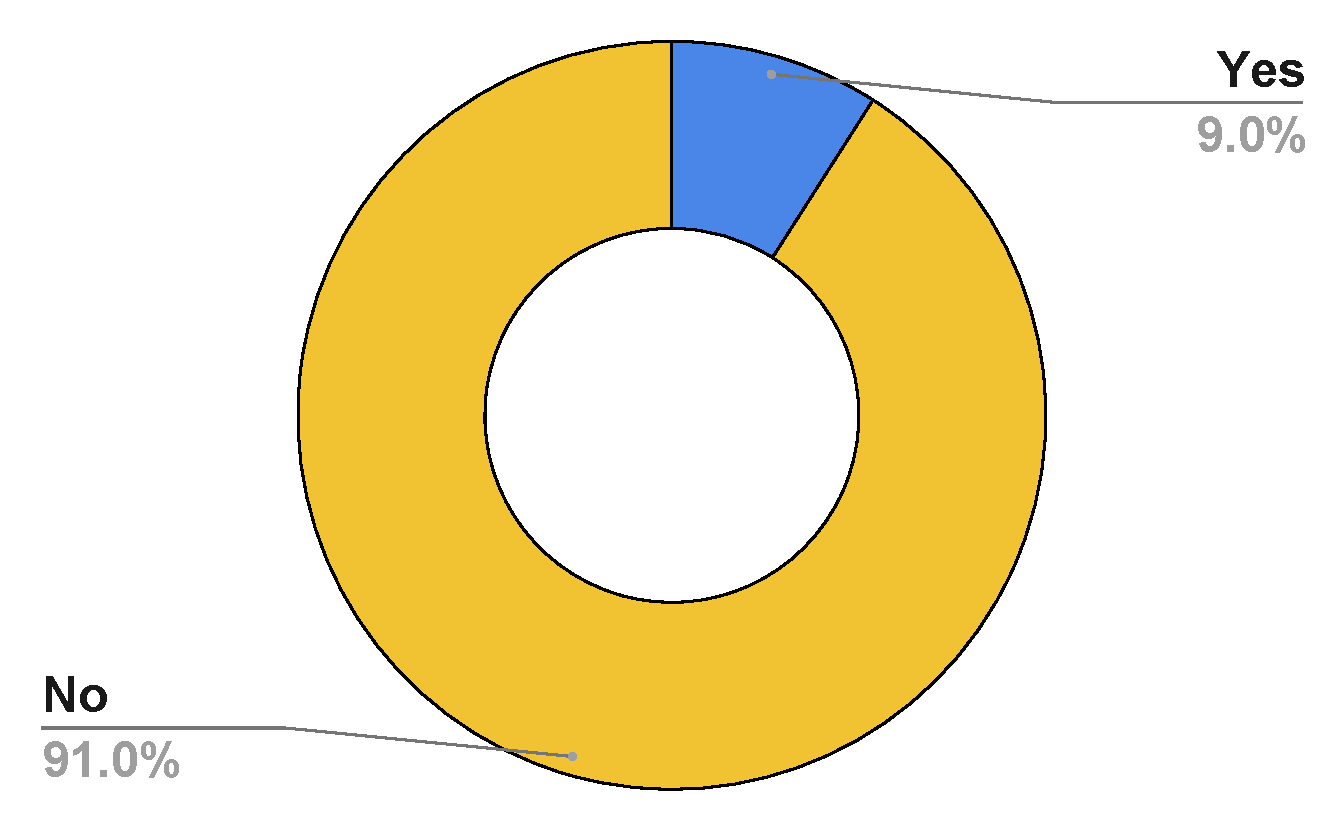
\includegraphics[width=0.6\columnwidth]{figures/social_message_majority.pdf}
    \caption{Distribution of the social message absence (No) and presence (Yes) labels in MM-AU}
    \label{Social_message_majority}
\end{figure}
\begin{figure*}[h!]
  \centering
  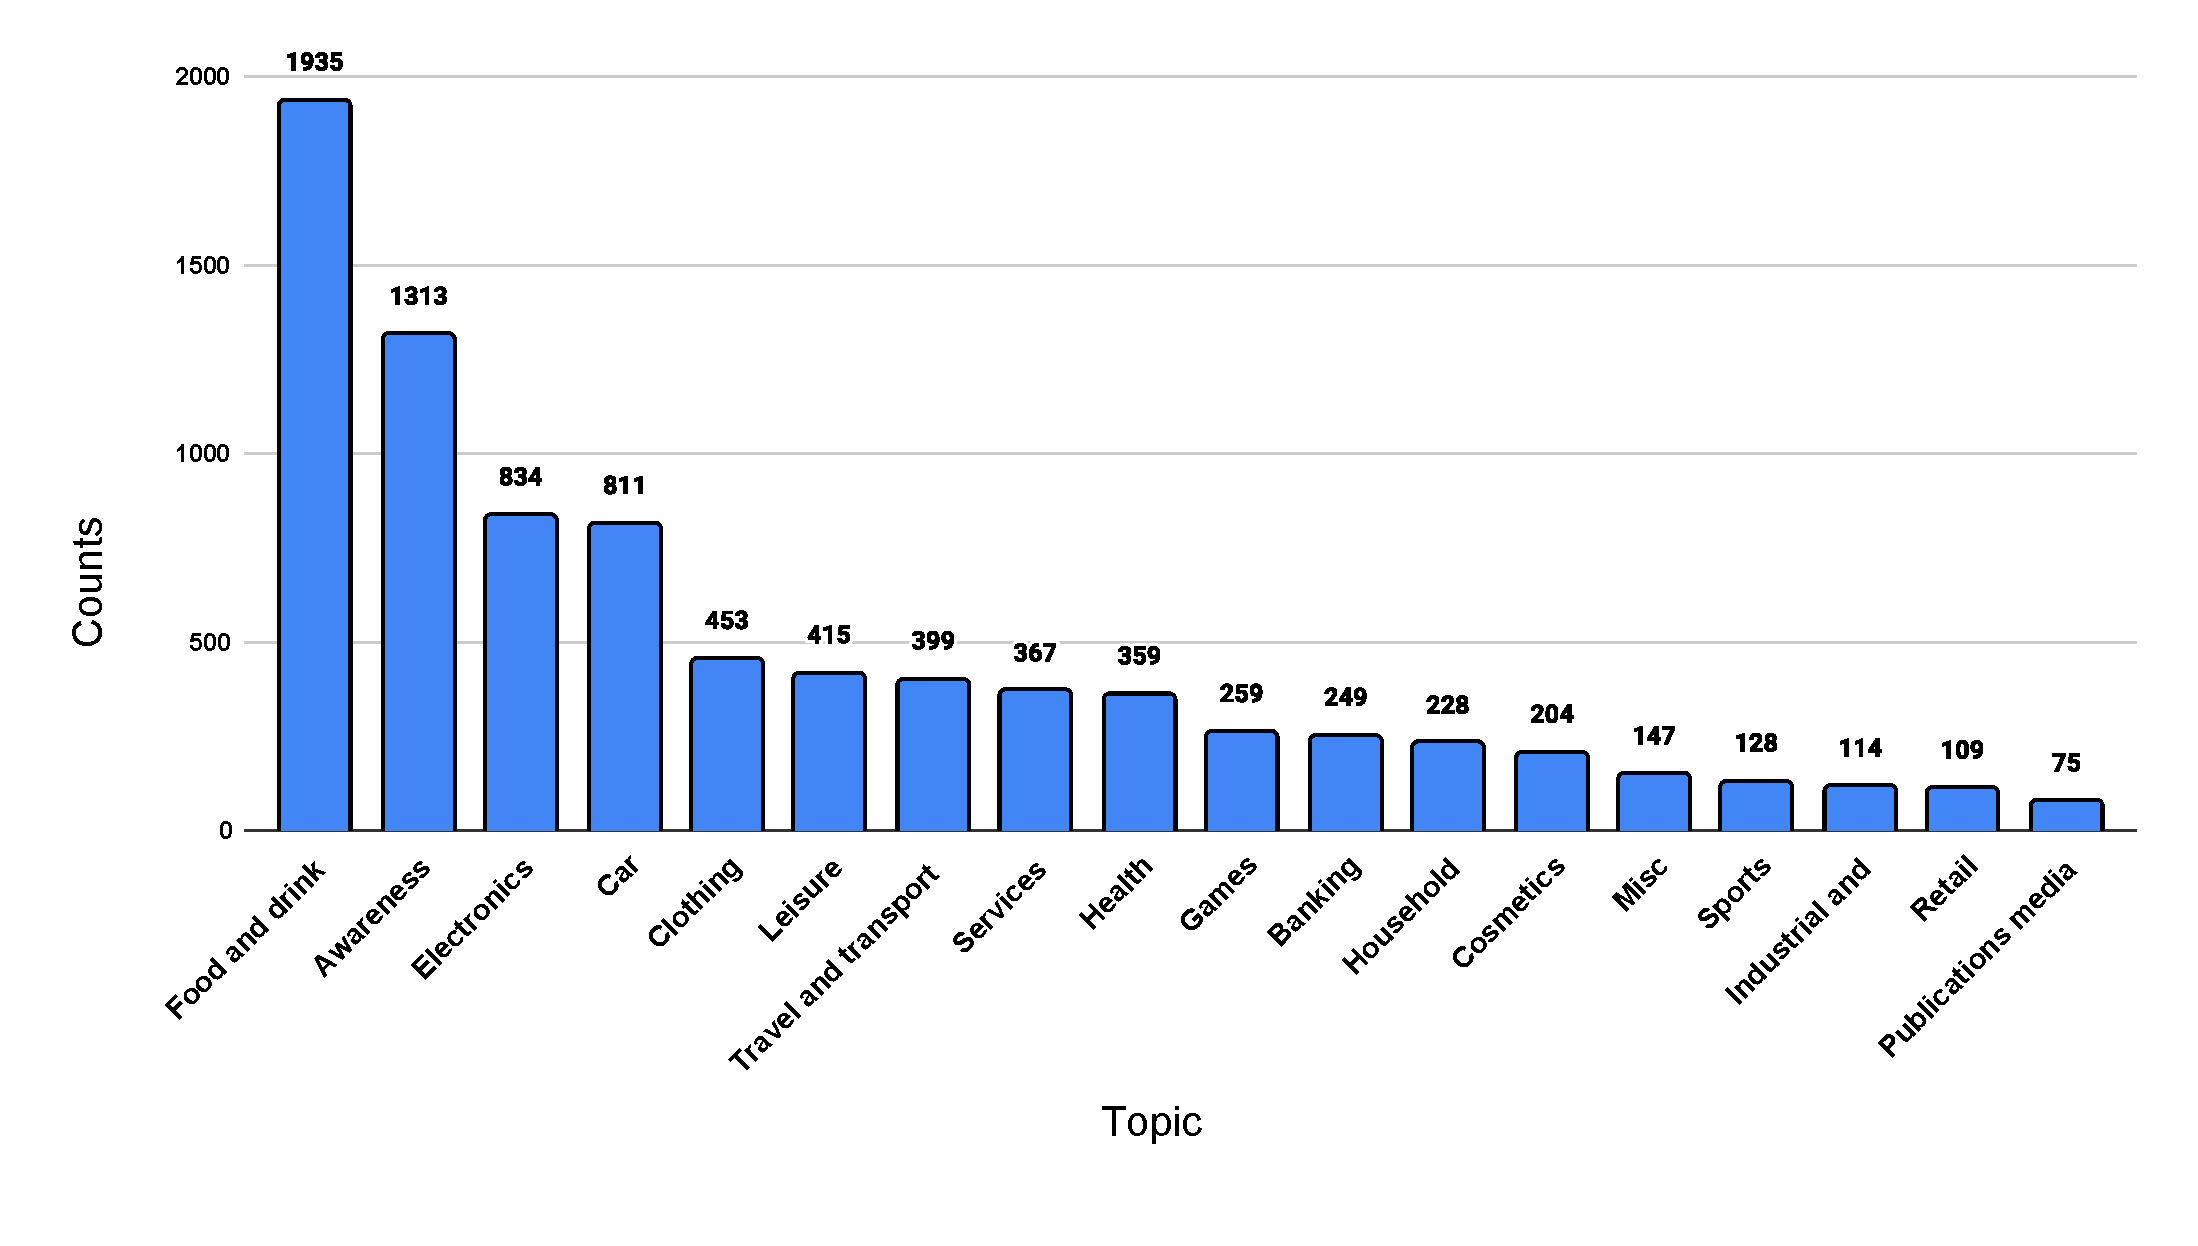
\includegraphics[width=\textwidth]{figures/topic_listing_new_pdf.pdf}
  \caption{Distribution of topics in MM-AU dataset}
  \label{topics}
\end{figure*}
The distribution of topics is shown in Fig~\ref{topics}, with Food and Drink, Awareness, and Electronics being the top-3 dominant categories. In the case of perceived tone labels, we obtain a high majority agreement among annotators in marking the start (\textbf{91.2\%}), middle (\textbf{91.6\%}), and the ending (\textbf{94.5\%}) segments of the videos with perceived tone labels. Since annotating the presence/absence of social messages is a comparatively less subjective task than perceived tone labeling, we obtain a majority agreement (\textbf{99\%}) among the annotators. In terms of tone labels for start, middle, and end segments, we can see from Fig~\ref{start_mid_end_tone}, that the dominant perceived tone for the advertisements is positive, with its share rising from \textbf{60.2\%} (start) to \textbf{81.3\%} (end). This can be explained due to the fact that advertisements are primarily designed to persuade viewers to buy certain products or act toward certain social issues. However, from Fig~\ref{start_mid_end_tone}, we can see that the share of negative tone labels increases from \textbf{15.5\%} to \textbf{19.6\%} due to the narrative structure of the ads, where the middle segment portrays negative elements like human suffering, environmental damage, etc to set up the final conclusion. From Fig~\ref{Social_message_majority}, we can see that \textbf{9.0\%} of the videos, i.e. 759 contain social messages, as marked by \textbf{Yes} label. Out of 759 videos, \textbf{62.5\%} exhibit transition in perceived tone with the share of negative tone rising from \textbf{32.3\%} to \textbf{43.3\%} in the middle segments.

% \begin{figure}[h!]
% \centering
% \subfloat[]{%
% 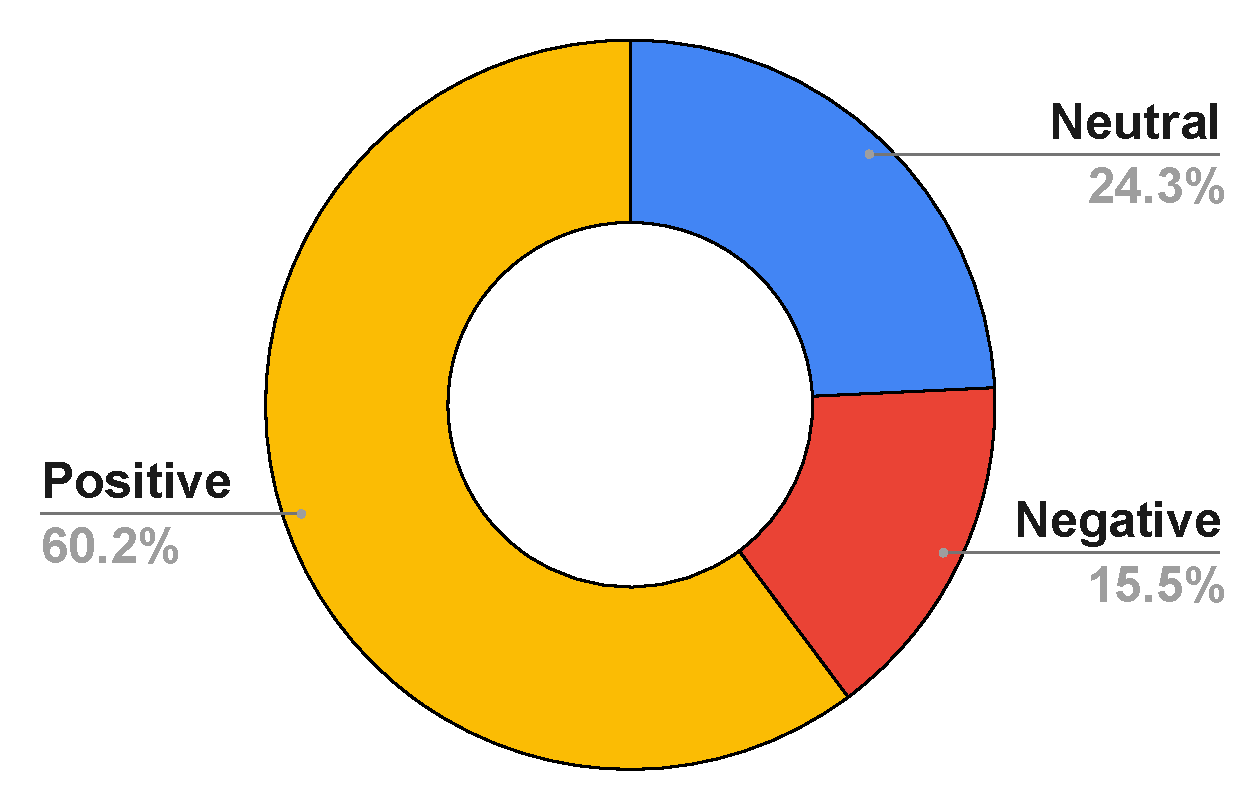
\includegraphics[width=0.33\textwidth]{figures/start_tone_majority.pdf}% 
% \label{start_tone}
% }
% \subfloat[]{%
% 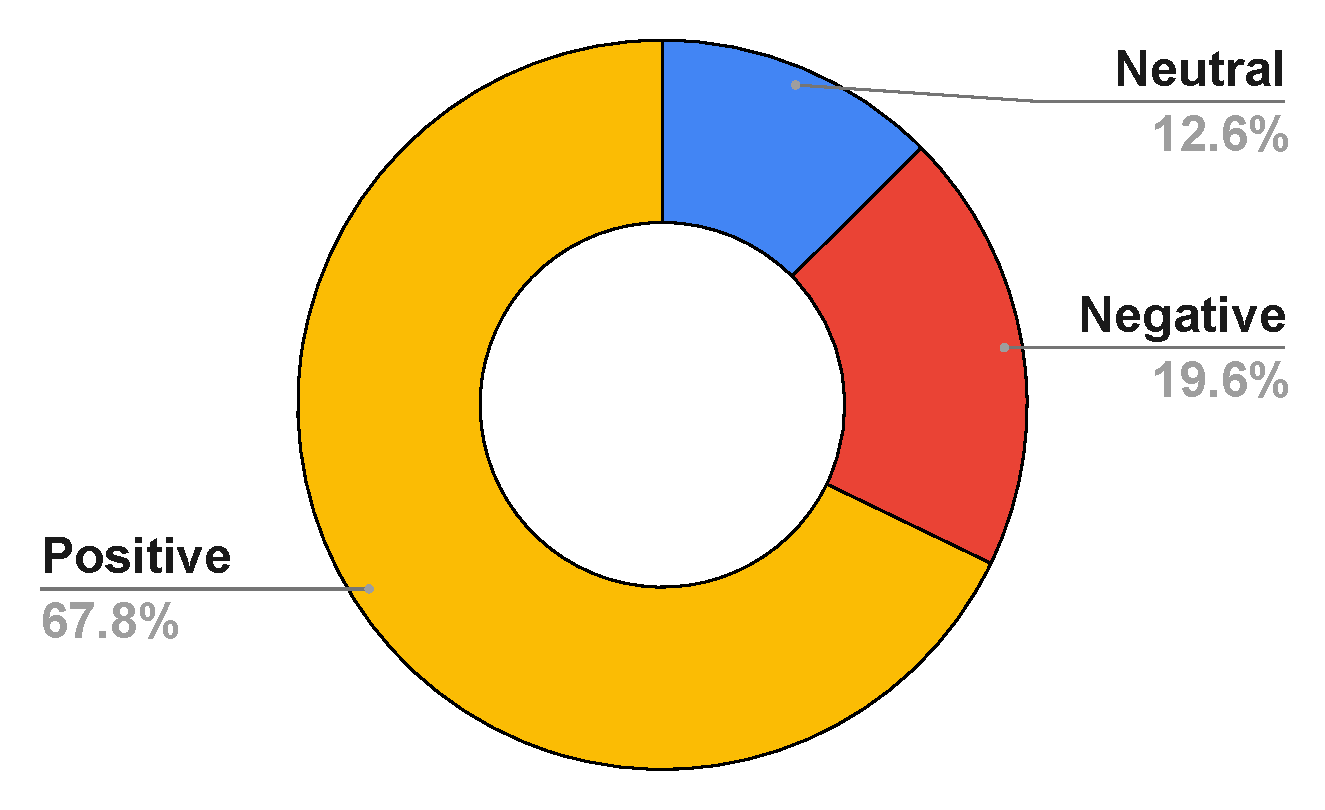
\includegraphics[width=0.33\textwidth]{figures/middle_tone_majority.pdf}%
% \label{mid_tone}
% }
% \subfloat[]{%
% 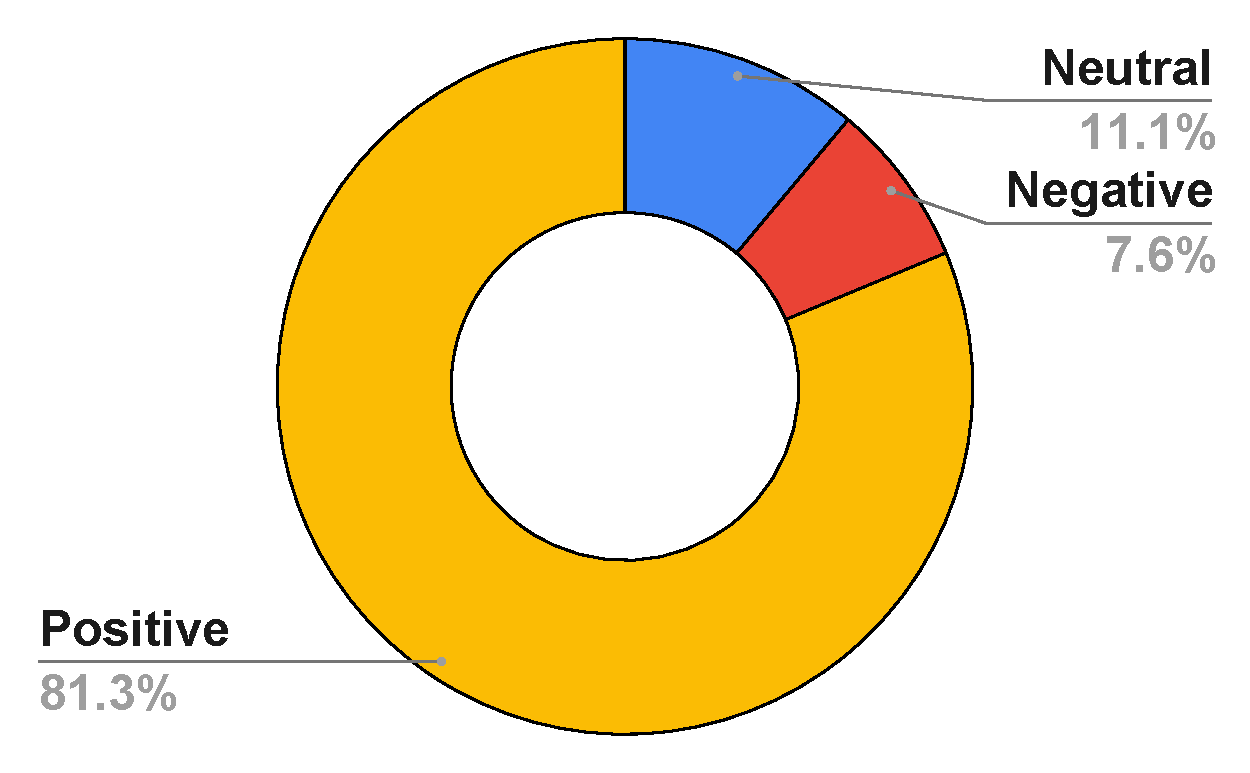
\includegraphics[width=0.34\textwidth]{figures/end_tone_majority.pdf}%
% \label{mid_tone}
% }
% \caption{Distribution of majority perceived tone labels (among 3 annotators) across (a) start, (b) middle, and (c) ending segments in MM-AU dataset (8399 videos) }
% \label{start_mid_end_tone}
% \end{figure}
\begin{figure}
\begin{subfigure}{.33\textwidth}
  \centering
  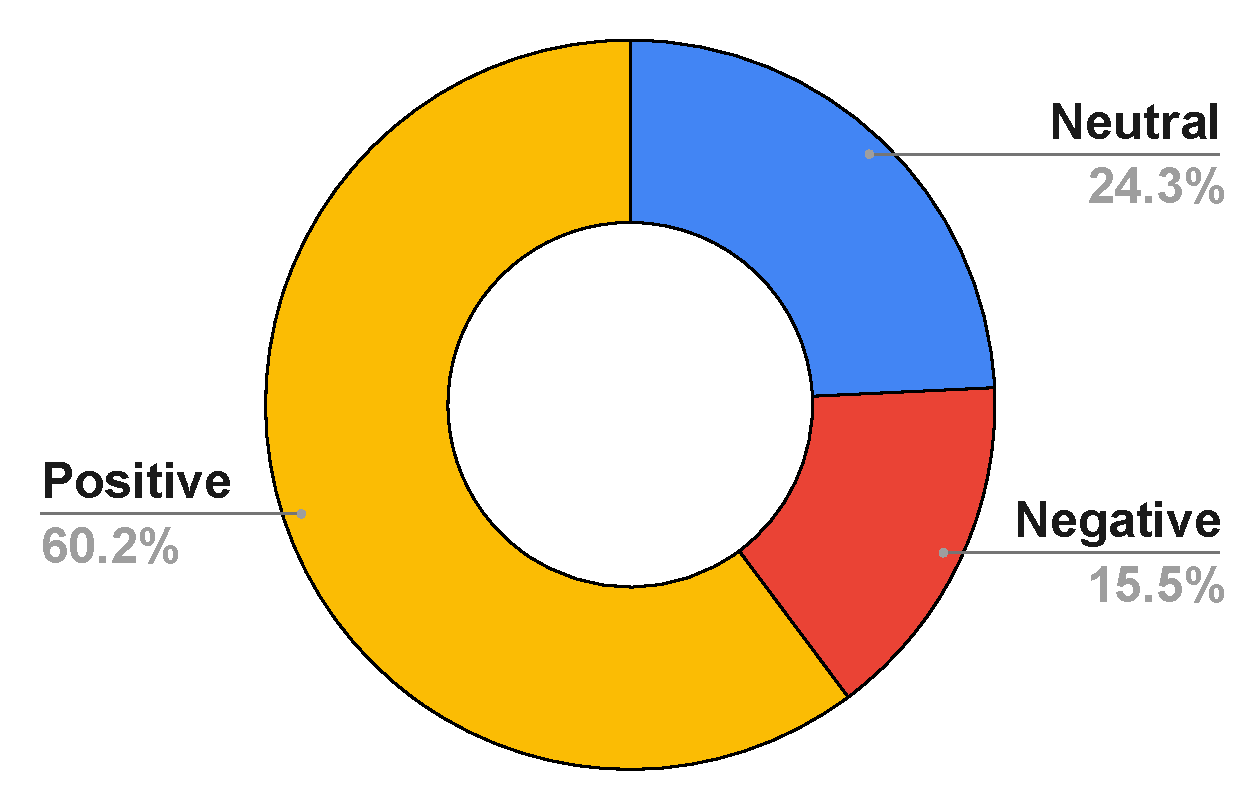
\includegraphics[width=.8\linewidth]{figures/start_tone_majority.pdf}
  \caption{Start segment}
  \label{start_tone}
\end{subfigure}%
\begin{subfigure}{.33\textwidth}
  \centering
  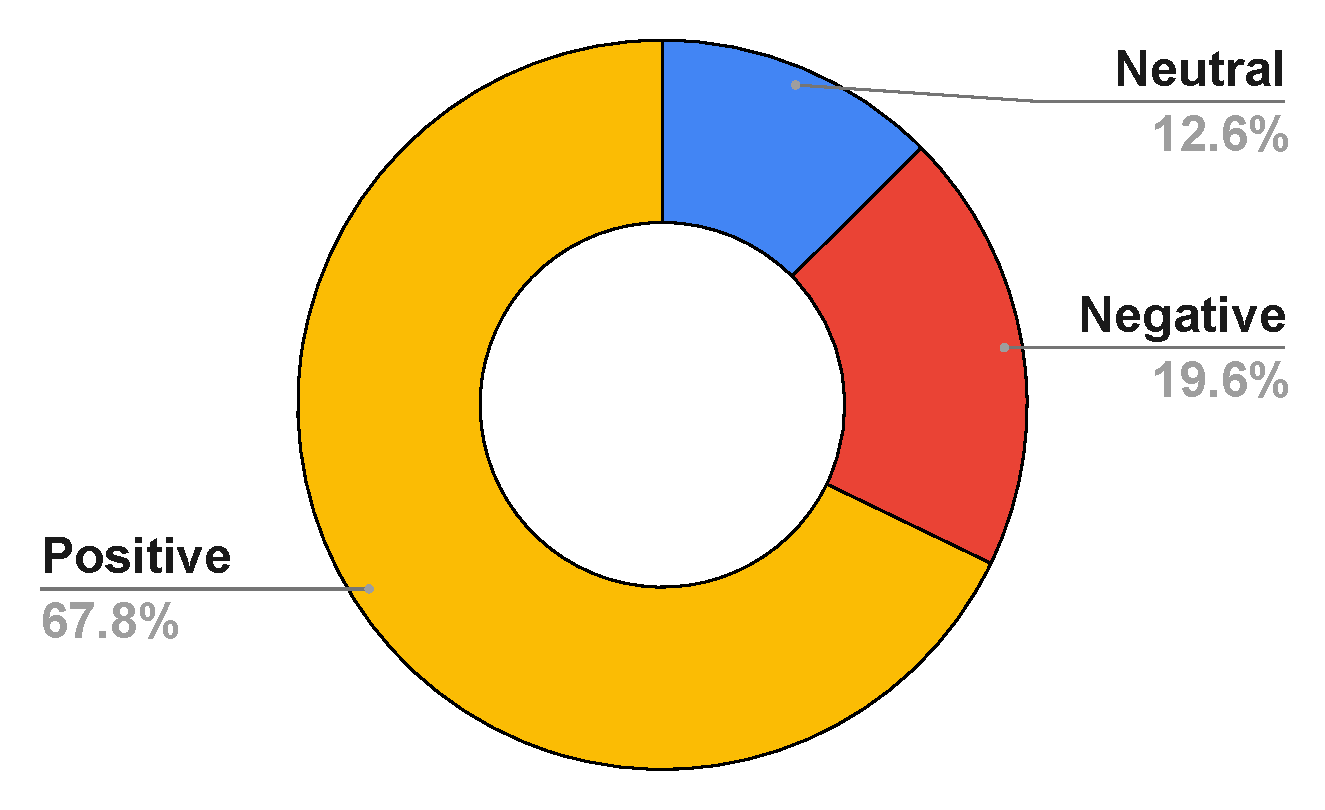
\includegraphics[width=.8\linewidth]{figures/middle_tone_majority.pdf}
  \caption{Middle segment}
  \label{mid_tone}
\end{subfigure}
\begin{subfigure}{.33\textwidth}
  \centering
  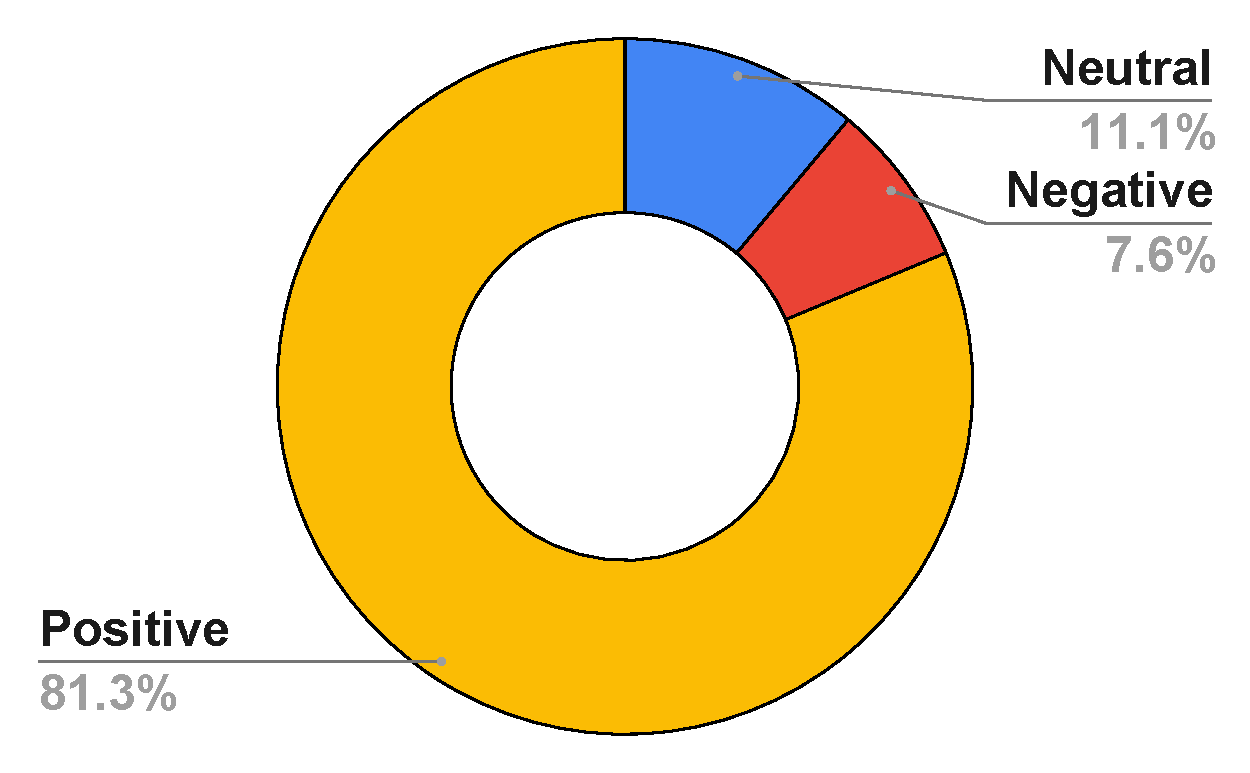
\includegraphics[width=.8\linewidth]{figures/end_tone_majority.pdf}
  \caption{End segment}
  \label{end_tone}
\end{subfigure}
\caption{Distribution of majority perceived tone labels (among 3 annotators) across (a) start, (b) middle, and (c) ending segments in MM-AU dataset (8399 videos) }
\label{start_mid_end_tone}
\end{figure}

\begin{figure}
\begin{subfigure}{.50\textwidth}
  \centering
  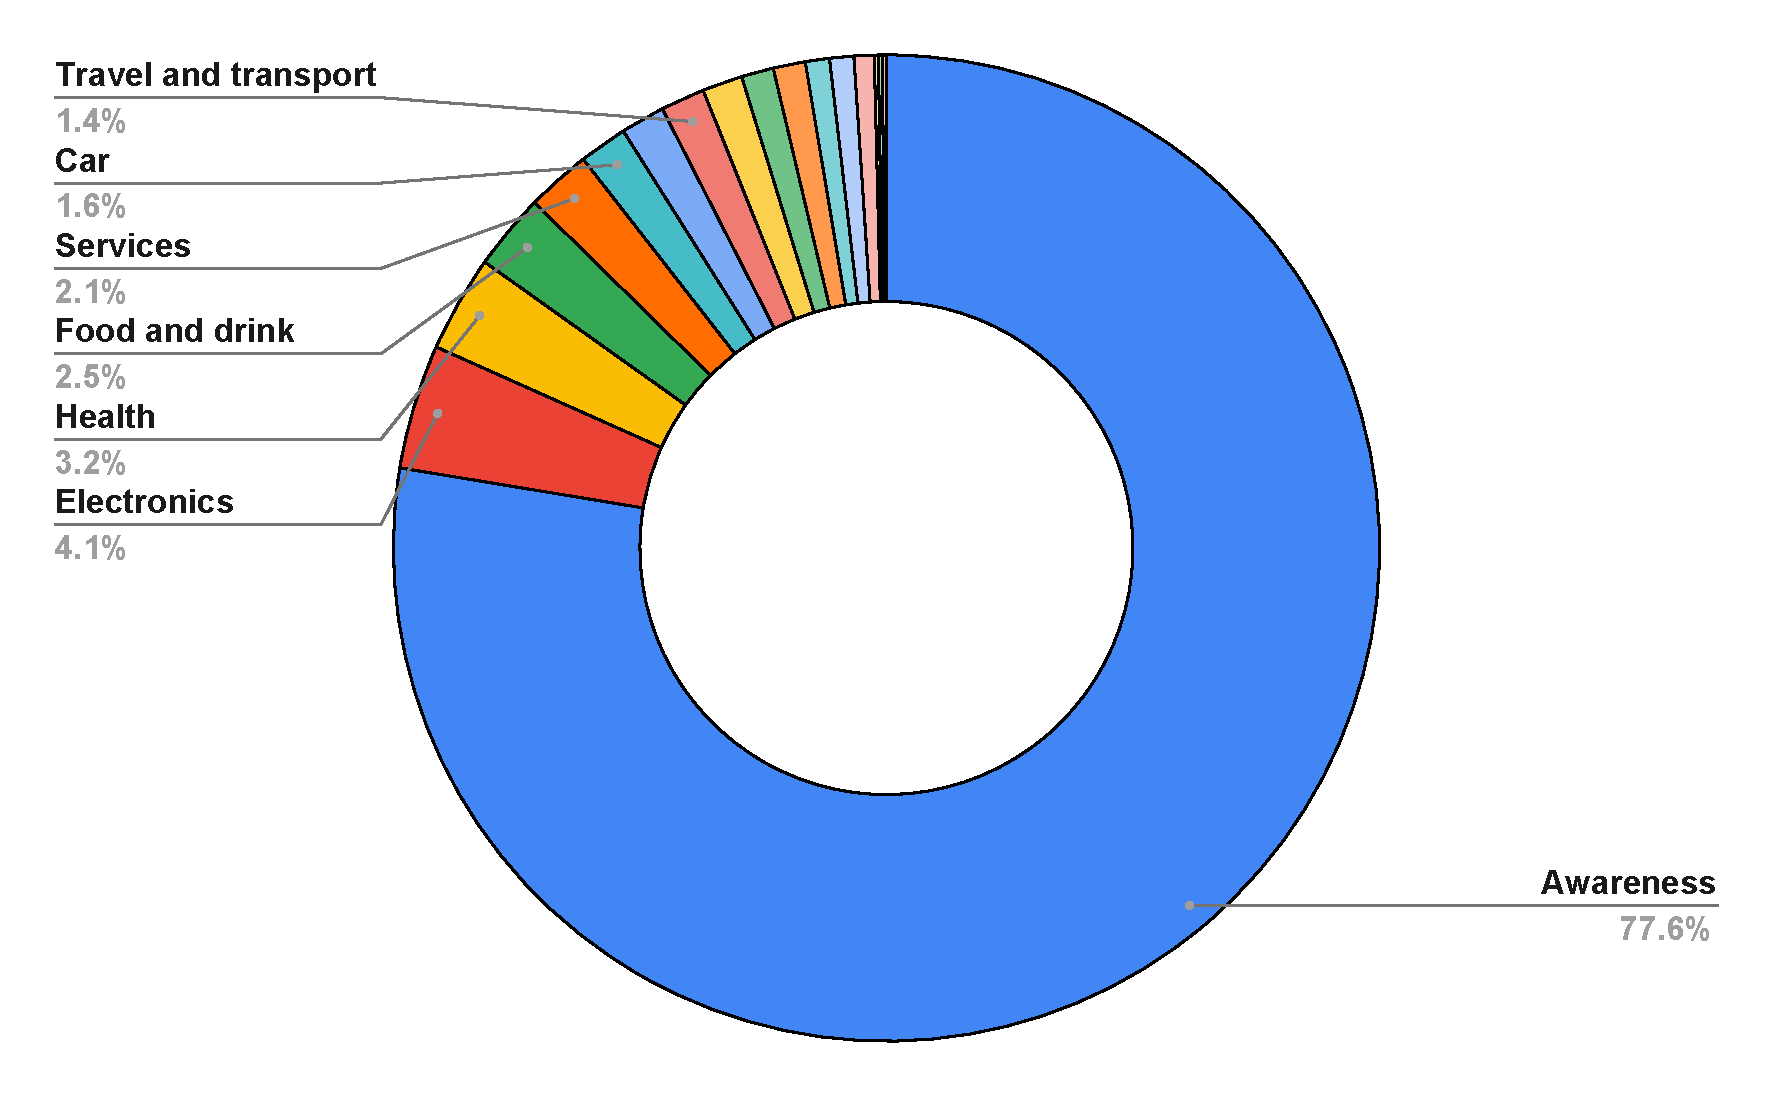
\includegraphics[width=\linewidth]{figures/topic_vs_social_message.pdf}
  \caption{Distribution of Topics wrt social message}
  \label{topic_social_message}
\end{subfigure}%
\begin{subfigure}{.50\textwidth}
  \centering
  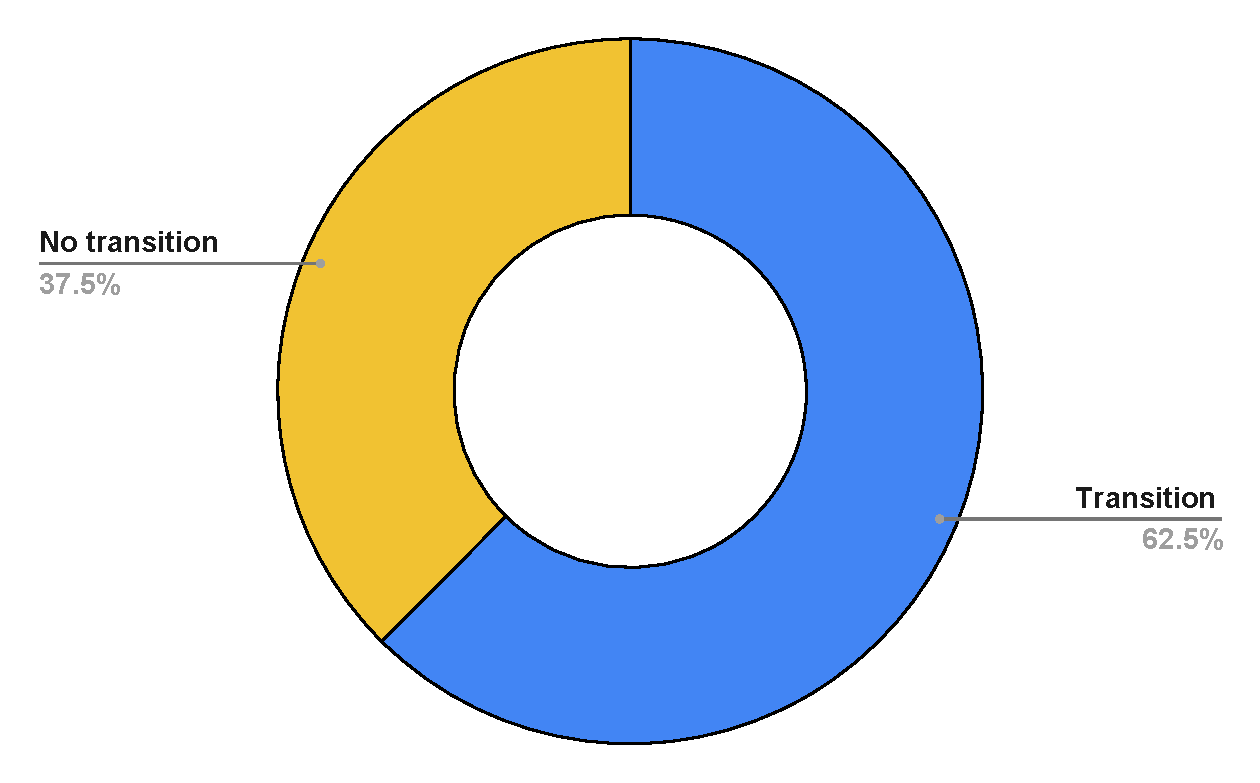
\includegraphics[width=\linewidth]{figures/transition_vs_social_message.pdf}
  \caption{Distribution of Tone transition wrt social message}
  \label{tone_transition_social_message}
\end{subfigure}
\caption{Distribution of topics and perceived tone transition across videos having the presence of social message (739 videos) in MM-AU dataset}
\label{topic_tone_transition_social_message}
\end{figure}
We further explore the intersection between the presence of social message and associated topics and tone transition (including tone labels for different segments of the video). From Fig \ref{topic_tone_transition_social_message} (a), we can see that out of 739 videos having social messages, \textbf{77.9\%} have \textbf{Awareness} as the associated topic label. The \textbf{Awareness} topic label includes subcategories related to social issues involving environmental damage, animal rights, smoking, alcohol abuse, domestic violence, refugee crisis, cyberbullying, etc. Further, as shown in Fig \ref{topic_tone_transition_social_message} (b), we observe a greater incidence of transitions in perceived tone (\textbf{62.5\%}) associated with videos having social messages. A detailed breakdown of segment-wise perceived tone labels for videos having social messages is shown in Fig \ref{start_mid_end_soc_msg_tone}. We can see an increase in the perceived negative tone from \textbf{32.3\%} to \textbf{43.3\%}. This can be attributed to the narrative structure of the advertisement videos having the presence of a social message where the middle segment primarily portrays negative elements i.e. environmental damage, human suffering etc to set up the conclusion.
\begin{figure}
\begin{subfigure}{.33\textwidth}
  \centering
  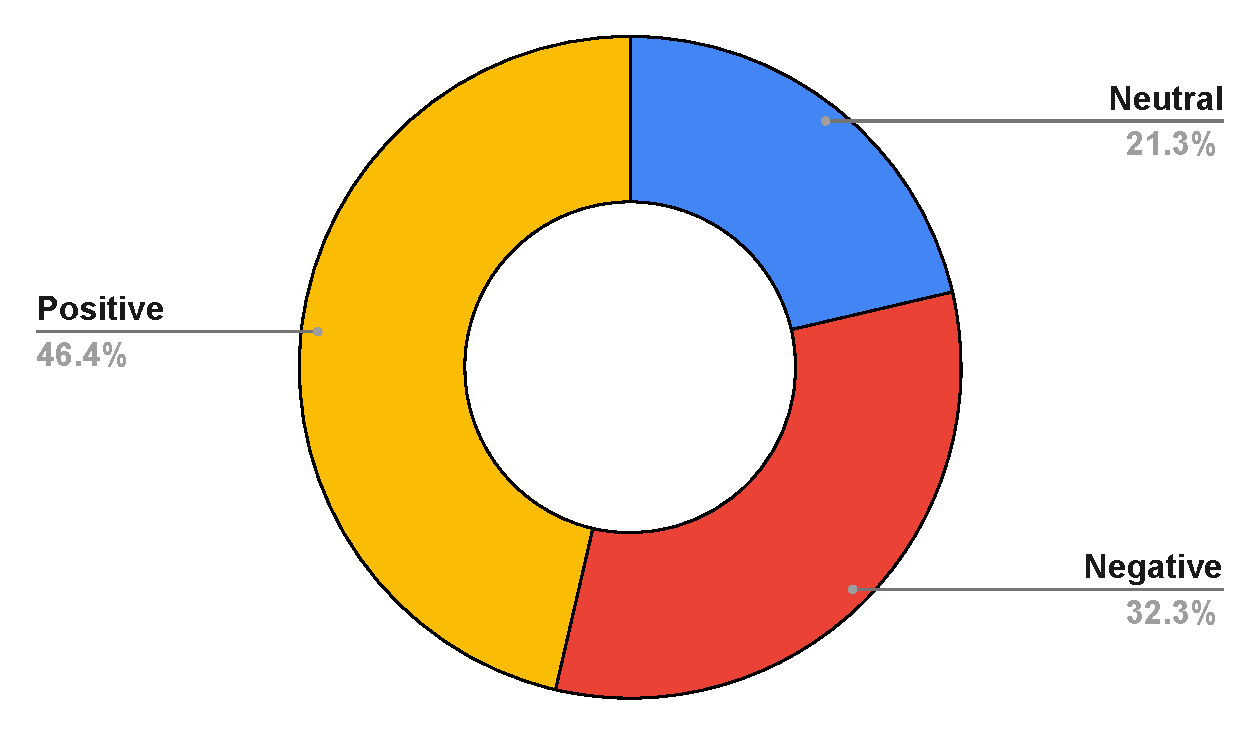
\includegraphics[width=\linewidth]{figures/start_tone_vs_social_message.pdf}
  \caption{Start segment}
  \label{start_tone_social_message}
\end{subfigure}%
\begin{subfigure}{.33\textwidth}
  \centering
  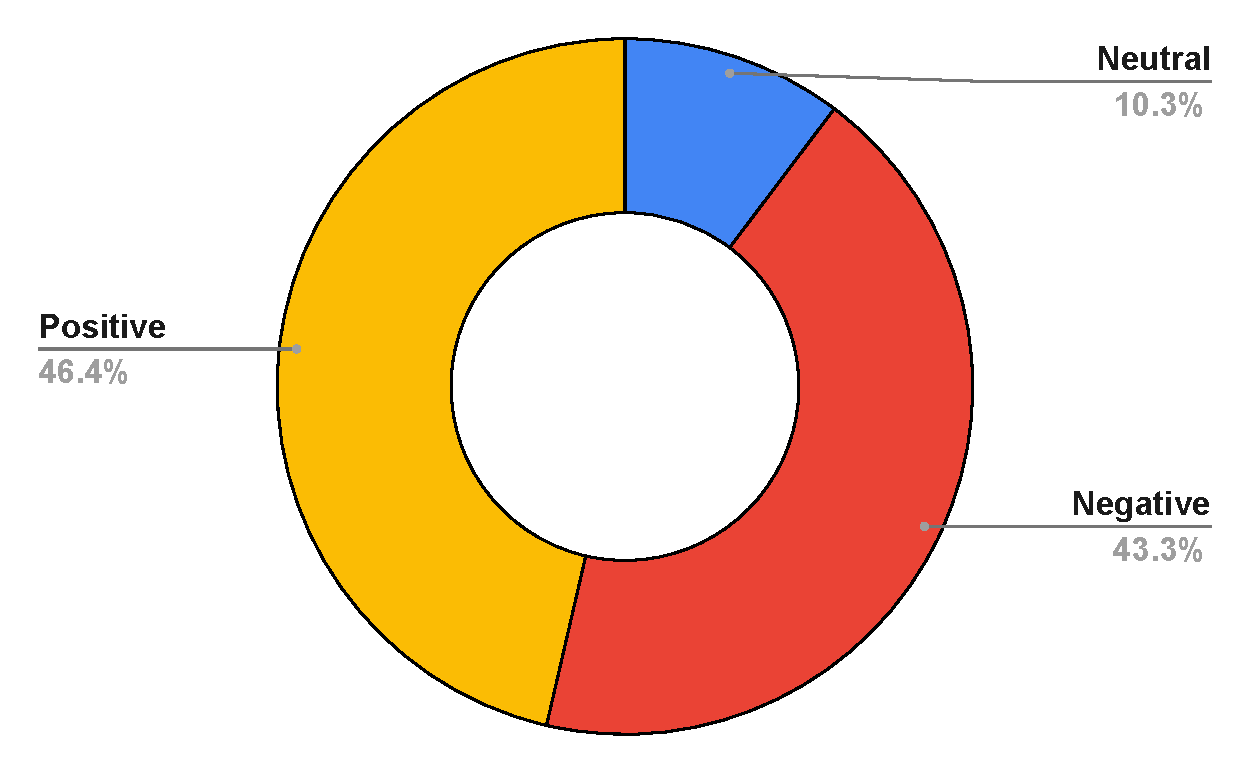
\includegraphics[width=\linewidth]{figures/middle_tone_vs_social_message.pdf}
  \caption{Middle segment}
  \label{mid_tone_social_message}
\end{subfigure}
\begin{subfigure}{.33\textwidth}
  \centering
  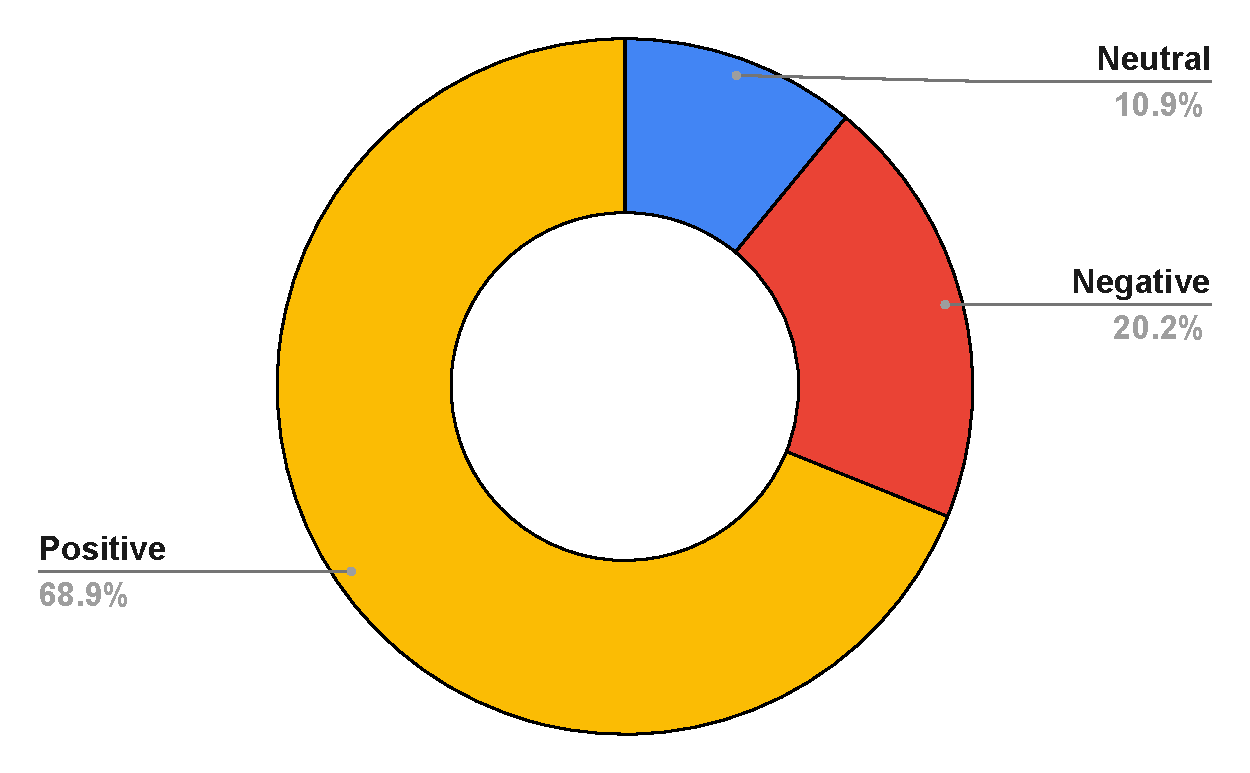
\includegraphics[width=\linewidth]{figures/ending_tone_vs_social_message.pdf}
  \caption{End segment}
  \label{end_tone_social_message}
\end{subfigure}
\caption{Distribution of perceived tone labels across the (a) start, (b) middle, and (c) ending segments in MM-AU dataset for videos having social message (739 videos) }
\label{start_mid_end_soc_msg_tone}
\end{figure}
\section{Task definition}
\textbf{\underline{Social message detection:}}
Based on the social message annotations (majority), the presence/absence of social message (SM) for $ith$ video is defined as:
\begin{equation}
  SM_{i} =
    \begin{cases}
      0 & \text{No (Absence of SM)}\\
      1 & \text{Yes (Presence of SM)}
    \end{cases}       
\end{equation}
Our aim is to learn a network $f_{SM}$ to predict social message presence/absence $\hat{SM}_{i}$ for the $ith$ video. The above definition results in 759 and 7640 videos marked with the presence  (1) and absence (0) of social messages, respectively.\\
\textbf{\underline{Tone transition:}}
Based on the start, middle, and end perceived tone labels (majority), we define the transition for $ith$ video as follows:
\begin{equation}
  Tr_{i} =
    \begin{cases}
      0 & \text{$Start_{i}=Mid_{i}=End_{i}$}\\
      1 & \text{else}
    \end{cases}       
\end{equation}
Our aim is to learn a network $f_{Tr}$ to predict binary tone transition $\hat{Tr}_{i}$ for the $ith$ video.
MM-AU dataset has 3854 and 4545 videos marked with Transition (1) and No Transition (0), respectively.\\
\textbf{\underline{Topic categorization:}}
For topic categorization, we aim to learn a multimodal network $f_{Topic}$ to predict $\hat{Topic}_{i}$ for the $ith$ video out of 18 target categories. 
\section{Context through multimodality}
In the case of advertisements, we utilize the available information with temporal and foreground contexts for macro-level understanding based on the previously mentioned tasks of topic categorization, social message detection, and tone transition. The context information can be processed through the modalities mentioned below:
\begin{itemize}
    \item \textbf{Temporal context:} Visual modality (shots with different camera viewpoints and semantic divisions), Audio modality 
      (Background music and audio events).
    \item \textbf{Foreground context:} Language modality (Narrations/descriptions through text transcripts).
\end{itemize}
\section{Multimodal context fusion}
For the input modalities $a$, $v$, $t$, we outline the separate context-guided fusion operations as follows:
\subsection{Foreground and temporal context fusion}
We outline the operations for foreground (\textbf{language}) and temporal (\textbf{visual}) context fusion as follows:
 \begin{align}
    \begin{split}
     e_{text}&=Text_{proj}(f_{text}(t))\\
     e_{vis}&=Vis_{proj}(f_{visual}(v)) \\ 
     TV_{logits}&=\mathbf{AvgPool}(\mathbf{{Tx}_{TV}}([e_{text};e_{vis}])) \\
    \end{split}
 \end{align}
 Here, $\mathbf{{Tx}_{TV}}$ is the text-visual fusion block used for combining foreground (\textbf{text}) and temporal (\textbf{visual}) contexts. $f_{visual}$ and $f_{text}$ refer to the pretrained visual and text encoders. The linear projection layers for visual and text modalities are denoted by $Vis_{proj}$ and $Text_{proj}$. 
 \begin{figure}[h!]
     \centering
     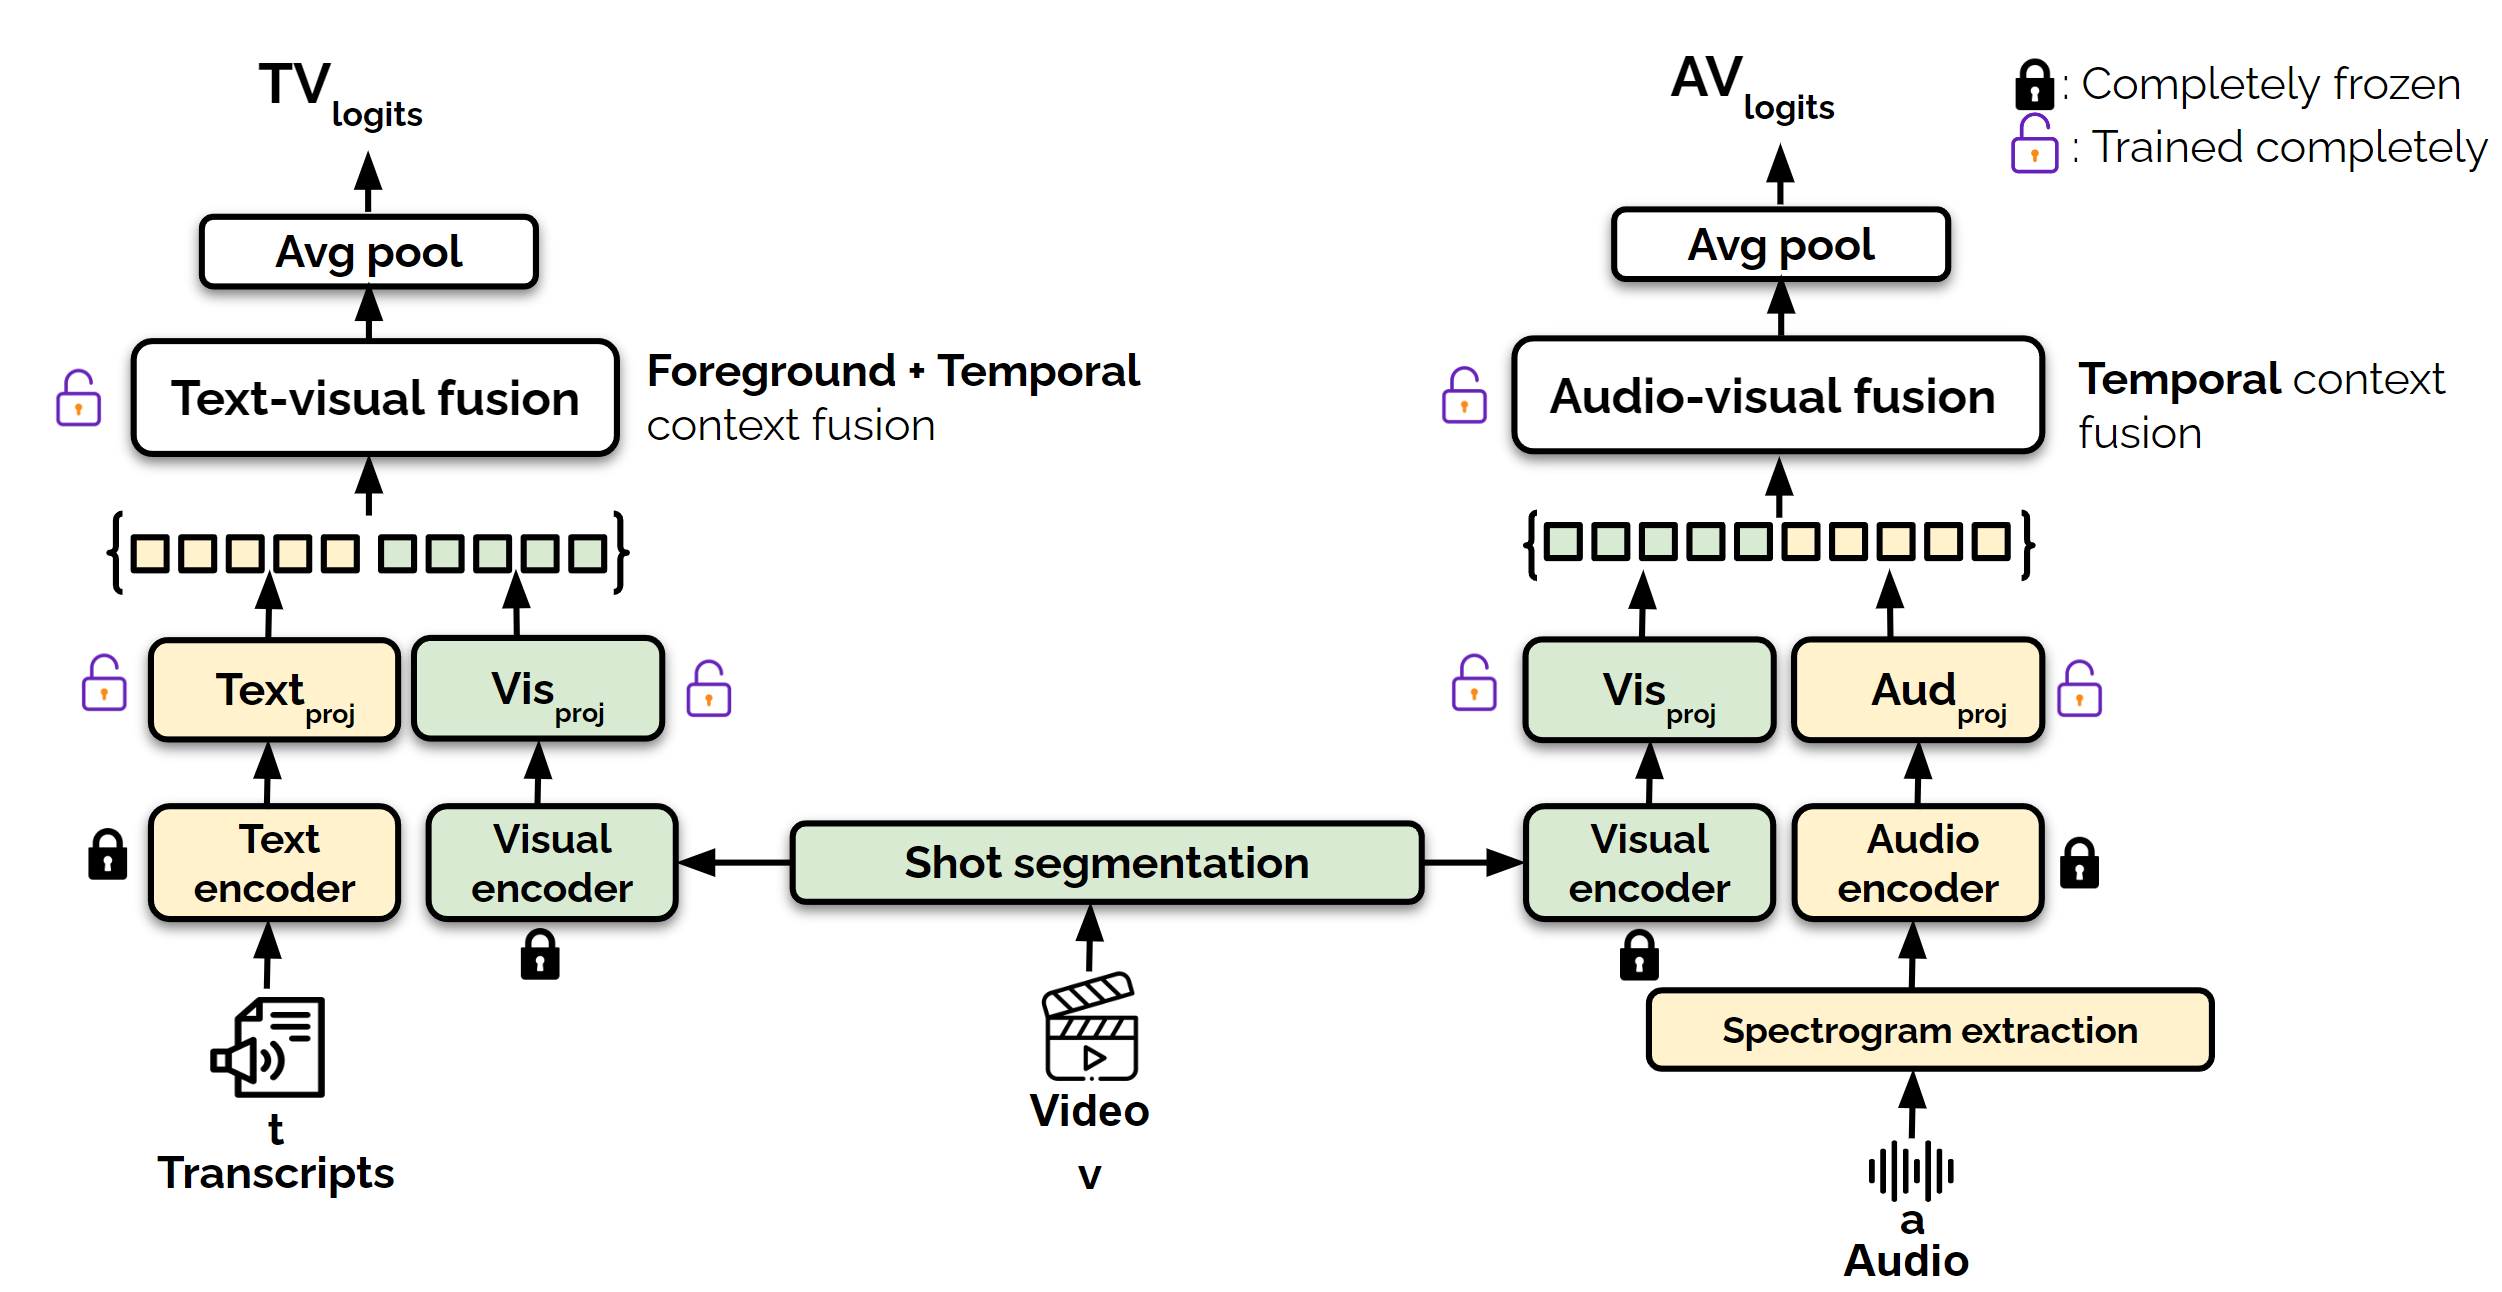
\includegraphics[width=\textwidth]{figures/ads_modeling_structure.png}
    \caption{Proposed architecture for the fusion of different modalities associated with temporal and foreground contexts. }
\end{figure}
\subsection{Temporal context fusion}
For the temporal context fusion block, we have the following sequence of operations:
\begin{align}
    \begin{split}
     e_{aud}&=Aud_{proj}(f_{aud}(a))\\
     e_{vis}&=Vis_{proj}(f_{visual}(v)) \\ 
     AV_{logits}&=\mathbf{AvgPool}(\mathbf{{Tx}_{AV}}([e_{aud};e_{vis}])) \\
    \end{split}
\end{align}
 Here, $\mathbf{{Tx}_{AV}}$ is the audio-visual fusion block used for combining temporal context information from (\textbf{audio}) and   (\textbf{visual}) modalities. $f_{visual}$ and $f_{aud}$ refer to the pretrained visual and audio encoders. The linear projection layers for visual and audio modalities are denoted by $Vis_{proj}$ and $Aud_{proj}$. 

 For the fusion blocks, we consider the PerceiverIO transformer architecture \cite{Jaegle2021PerceiverIA} due to the following reasons:

 \begin{itemize}
    \item \textbf{Reduction in operational complexity:} In the case of PerceiverIO, the input embedding matrix having a significantly large sequence length is mapped to a limited group of latent vectors followed by attention operation on the latent vectors. This decreases the operational complexity of the attention operation. In Fig \ref{Perceiver}, $N$ is smaller than input sequence length $M$.
    \item \textbf{Generalization to a wide variety of inputs:} PerceiverIO architecture has been shown to be highly generalizable to a wide variety of inputs, including video, audio, and point clouds.
 \end{itemize}

In our proposed approach, we train the fusion blocks $\mathbf{{Tx}_{AV}}$ and $\mathbf{{Tx}_{TV}}$ separately due to overfitting issues faced while using a single fusion block for three modalities. Further, the combinations of different modalities (\textbf{audio-visual}) and (\textbf{text-visual}) contain complementary information that further improves macro-level understanding across the tasks in MM-AU benchmark. In order to capture the complementary information, we perform logit fusion by freezing the $\mathbf{{Tx}_{AV}}$ and $\mathbf{{Tx}_{TV}}$ blocks using the following strategies:

\begin{itemize}
    \item \textbf{A-max:} $pred_{class}=\argmaxA_i (TV_{logits}(i)+AV_{logits}(i))/2$
    \item \textbf{D-max:} $pred_{class}=\argmaxA_i max\{(TV_{logits}(i),AV_{logits}(i))\}$
\end{itemize}
Here $i \in \{1,...Class\}$, where $Class$ refers to the number of classes associated with the task.

 \begin{figure}
 \centering
    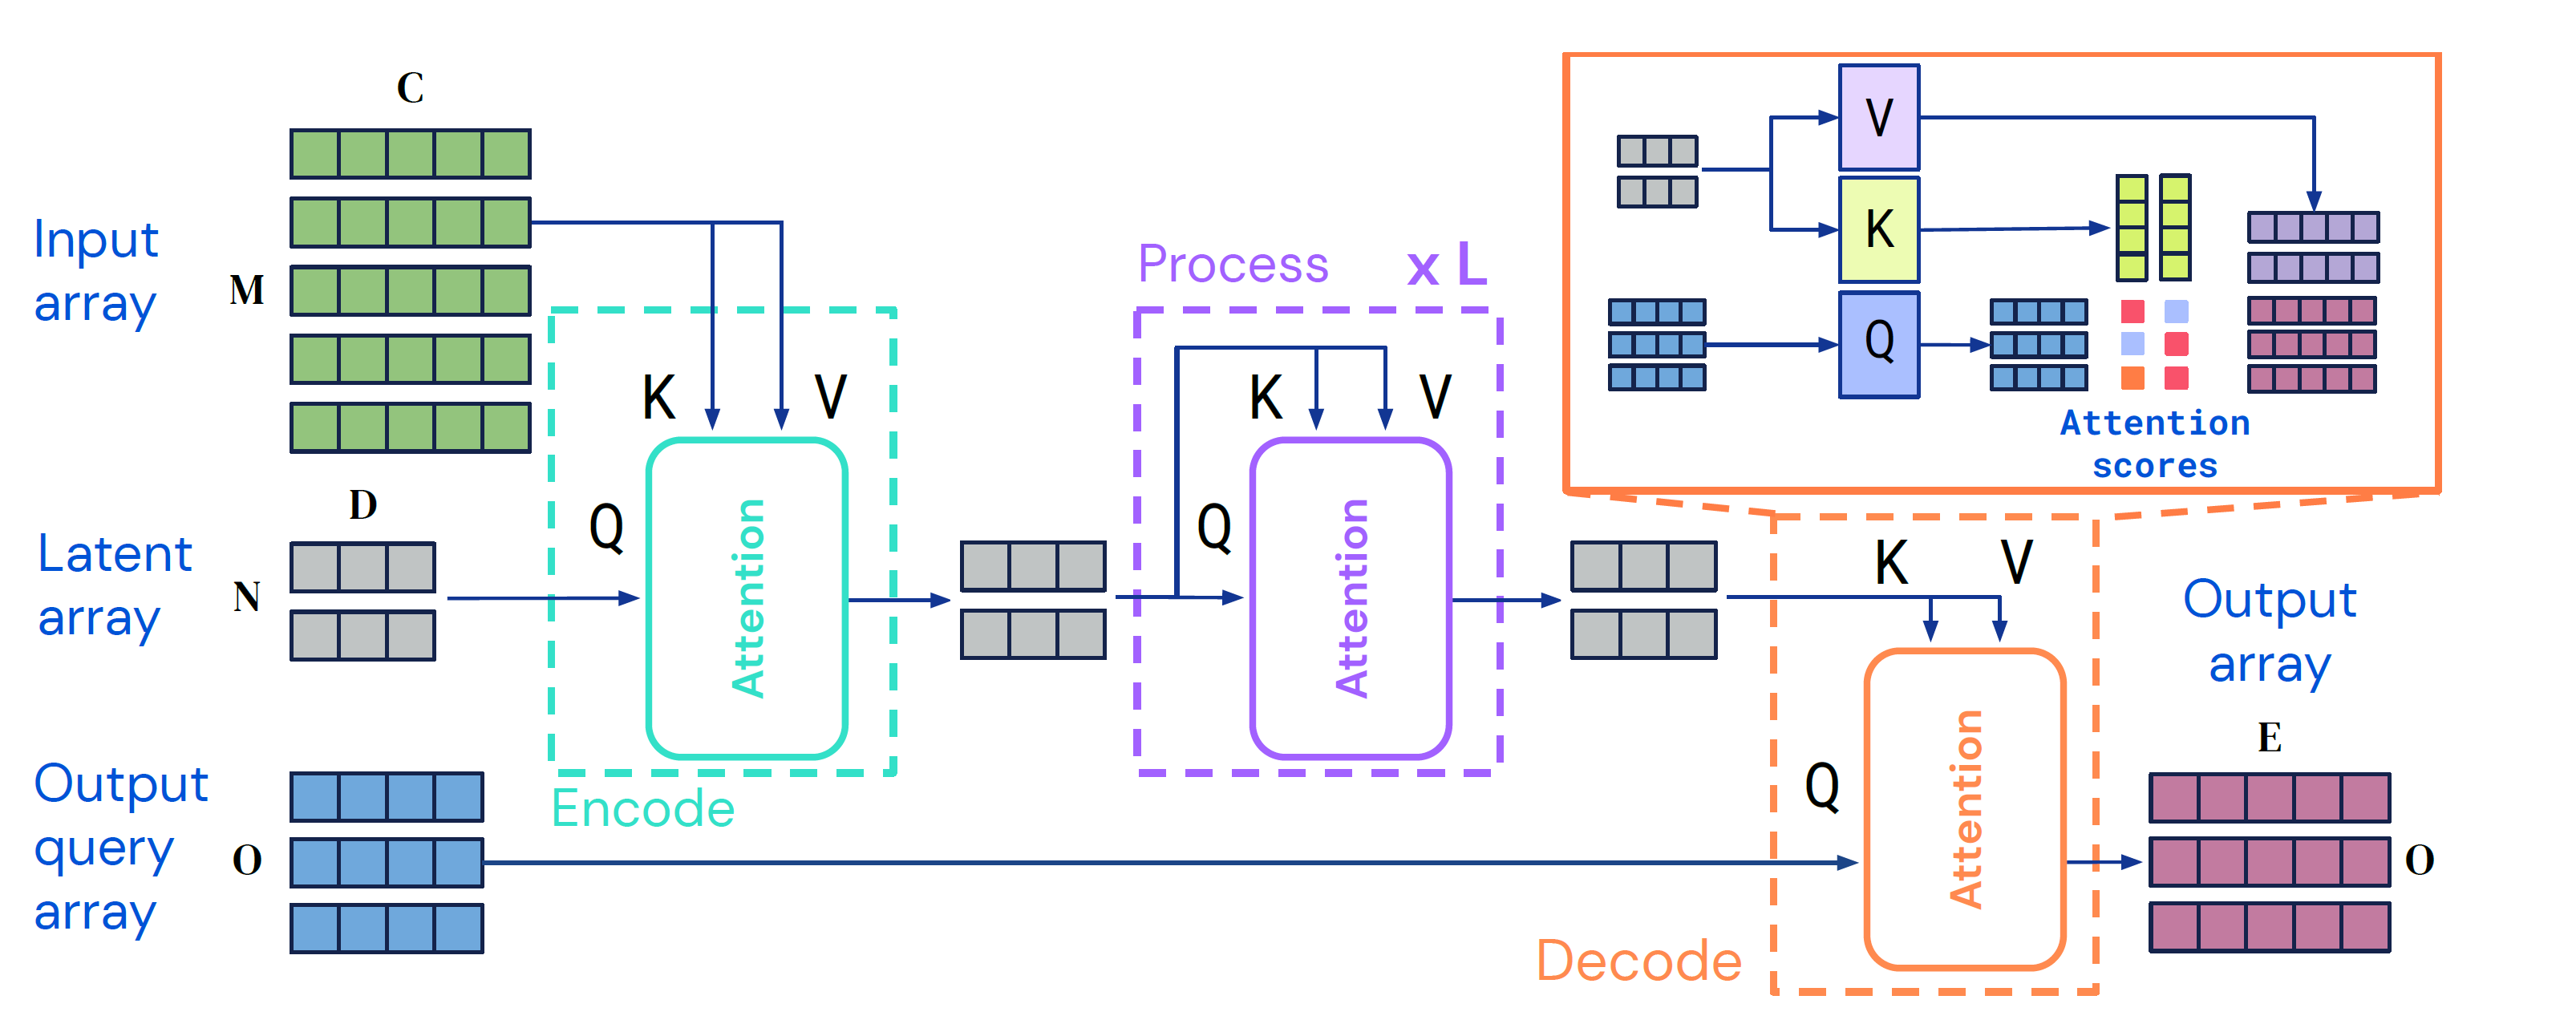
\includegraphics[width=0.8\textwidth]{figures/perceiver_architecture.png}
    \caption{PerceiverIO architecture \cite{Jaegle2021PerceiverIA}}
    \label{Perceiver}
 \end{figure}

\section{Experiments}
\subsection{Experimental Setup}
For training, validation, and testing purposes, we consider a split of 5877 (\textbf{70\%}), 830 (\textbf{10\%}), and 1692 (\textbf{20\%}) videos. The modality-specific details are as follows:

\textbf{\underline{Visual:}} For the visual modality, we segment the videos into shots using \texttt{PySceneDetect}\footnote{https://github.com/Breakthrough/PySceneDetect}. We use the shots to extract frame-wise features at 4 fps using CLIP's \cite{Radford2021LearningTV} pretrained visual encoder ($f_{visual}$), \texttt{ViT-B/32}. Further, we average pool the frame-wise visual representations to obtain shot representations. For modeling temporal context information through visual modality, we consider the shot as the basic unit due to its ability to capture short-term temporal variations. \\
 \textbf{\underline{Text:}} For the text modality, we use Whisper \cite{Radford2022RobustSR} multilingual model (\texttt{large}) to extract the transcripts.  We translate the multilingual transcripts to English using \texttt{GPT-4} \cite{OpenAI2023GPT4TR} (\textit{temp=0.02, max tokens=2048}) by providing the following translation-specific prompt: \textit{\textbf{Please provide an English translation of this transcript}}. We use the pretrained BERT\cite{Devlin2019BERTPO} model as the text encoder ($f_{text}$). The translated transcripts contain details about the foreground context in terms of narrations regarding interactions.\\
 \textbf{\underline{Audio:}} For the audio modality, we use the Audio-Spectrogram transformer (AST) \cite{gong21b_interspeech} model ($f_{audio}$) pretrained on AudioSet \cite{Gemmeke2017AudioSA} for extracting features at 10-sec intervals with a step size of 512.  \\
 We conduct our experiments in a distributed manner using the Pytorch \cite{Paszke2019PyTorchAI} framework on 4 2080ti GPUs. We use \textbf{accuracy} and \textbf{macro-F1} for evaluation metrics.
 \subsection{Language-based reasoning}
We investigate the zero-shot capabilities of foundational large language models \cite{Zhao2023ASO} by applying \texttt{GPT-4} \cite{OpenAI2023GPT4TR}, \texttt{Opt-IML} \cite{Iyer2022OPTIMLSL}, \texttt{Flan-T5} (XXL,XL,L) \cite{Chung2022ScalingIL} and \texttt{Alpaca} \cite{alpaca} on the translated transcripts. We report the results on 1670 non-empty transcripts out of the test split of 1692 samples for zero-shot evaluation. For \texttt{GPT-4} we use the following task-specific prompts:
\begin{itemize}
    \item \textbf{SM:} \textit{An advertisement video has a social message if it provides awareness about any social issue. Example of social issues: gender equality, drug abuse, police brutality, workplace harassment, domestic violence, child labor, environmental damage, homelessness, hate crimes, racial inequality etc. Based on the given text transcript, determine if the advertisement has any social message. Please provide answers in \textbf{Yes} and \textbf{No.}}
    \item \textbf{TT:} \textit{Based on the given text transcript from the advertisement, determine if the advertisement has any transitions in tones. Possible tone labels are: positive, negative, and neutral. Please respond by saying \textbf{Transition} or \textbf{No transition}}
    \item \textbf{Topic:} \textit{Associate a single topic label with the transcript from the given set: $<$Topic list$>$}
\end{itemize}
Here \textbf{SM}, \textbf{TT}, and \textbf{Topic} refer to the benchmark tasks of Social message detection, tone transition, and topic categorization. $<$Topic list$>$ refers to the condensed list of 18 topic categories curated for the MM-AU benchmark. Further details about the prompting strategies are included as part of the Appendix (\ref{app:language_baselines}).
\subsection{Unimodal and Multimodal context fusion}
For the supervised unimodal baselines we consider the following model choices:
\begin{itemize}
    \item \textbf{LSTM \cite{lstm}:} 2 layers and hidden dimension = 256
    \item \textbf{MHA \cite{transformers}:} 4 layers, 4 heads and hidden dimension = 256
\end{itemize}
For the fusion blocks $\mathbf{{Tx}_{AV}}$ and $\mathbf{{Tx}_{TV}}$, we adopt a lightweight PerceiverIO structure composed of 4 encoder layers, 16 latent vectors, 8 heads, and a hidden latent dimensionality of 256. We use binary cross-entropy for social message and tone transition detection tasks and multi-class cross-entropy for topic categorization. For training the unimodal and multimodal models, we use a batch size of 16 with Adam \cite{Kingma2015AdamAM} or AdamW \cite{AdamW} as optimizers and $lr \in \{1e-4, 1e-5\}$. While training the supervised models, we fix the maximum sequence lengths for visual(shots), audio, and text modalities at 35, 14, and $\{256,512\}$, respectively. During multimodal fusion, when text is missing in the transcripts due to the absence of speech, we replace the text with a string of \texttt{[MASK]} tokens.

\section{Results}

\subsection{Language-only reasoning}

\begin{table}[h!]
\resizebox{\columnwidth}{!}{
\begin{tabular}{|cc|cc|cc|cc|}
\hline
\multicolumn{2}{|c|}{\textbf{Configurations}}                & \multicolumn{2}{c|}{\textbf{SM}}                & \multicolumn{2}{c|}{\textbf{TT}}                & \multicolumn{2}{c|}{\textbf{Topic}}             \\ \hline
\multicolumn{1}{|c|}{\textbf{Model}}       & \textbf{Params} & \multicolumn{1}{c|}{\textbf{Acc}} & \textbf{F1} & \multicolumn{1}{c|}{\textbf{Acc}} & \textbf{F1} & \multicolumn{1}{c|}{\textbf{Acc}} & \textbf{F1} \\ \hline
\multicolumn{1}{|c|}{\textbf{GPT-4 \textcolor{red}{\cite{OpenAI2023GPT4TR}}}}       & $NA^{*}$             & \multicolumn{1}{c|}{\textbf{87.6}}         & \textbf{65.66}    & \multicolumn{1}{c|}{\textbf{58.56}}        & \textbf{58.33}       & \multicolumn{1}{c|}{\textbf{33.29}}       & \textbf{29.21}       \\ \hline
\multicolumn{1}{|c|}{\textbf{Flan-T5-XXL \textcolor{red}{\cite{Chung2022ScalingIL}}}} & 11B             & \multicolumn{1}{c|}{85.69}        & 62.7        & \multicolumn{1}{c|}{54.79}        & 44.15       & \multicolumn{1}{c|}{30.54}        & 24.23       \\ \hline
\multicolumn{1}{|c|}{\textbf{Flan-T5-XL \textcolor{red}{\cite{Chung2022ScalingIL}}}}  & 3B              & \multicolumn{1}{c|}{65.51}        & 49.31       & \multicolumn{1}{c|}{54.67}        & 42.39       & \multicolumn{1}{c|}{27.18}        & 24.1        \\ \hline
\multicolumn{1}{|c|}{\textbf{Alpaca  \textcolor{red}{\cite{alpaca}}}}      & 7B              & \multicolumn{1}{c|}{10.77}        & 10.56       & \multicolumn{1}{c|}{46.88}        & 39.1        & \multicolumn{1}{c|}{11.19}        & 11.68       \\ \hline
\multicolumn{1}{|c|}{\textbf{Opt-IML \textcolor{red}{\cite{Iyer2022OPTIMLSL}}}}     & 1.3B            & \multicolumn{1}{c|}{37.07}        & 32.49       & \multicolumn{1}{c|}{54.37}        & 35.22       & \multicolumn{1}{c|}{22.22}        & 19.08       \\ \hline
\multicolumn{1}{|c|}{\textbf{Flan-T5-L \textcolor{red}{\cite{Chung2022ScalingIL}}}}   & 780M            & \multicolumn{1}{c|}{8.32}         & 7.76        & \multicolumn{1}{c|}{54.43}        & 35.25       & \multicolumn{1}{c|}{26.82}        & 19.42       \\ \hline
\multicolumn{1}{|c|}{Random Baseline}      & \textbf{-}           & \multicolumn{1}{c|}{49.57}        & 39.61       & \multicolumn{1}{c|}{49.95}        & 49.88        & \multicolumn{1}{c|}{5.71}        & 4.71 \\ \hline
\multicolumn{1}{|c|}{Majority Baseline}      & \textbf{-}           & \multicolumn{1}{c|}{90.96}        & 47.63       & \multicolumn{1}{c|}{54.11}        & 35.11        & \multicolumn{1}{c|}{23.04}        & 2.08 \\ \hline
\end{tabular}
}
\caption{Zero shot performance comparison between various LLMs on MM-AU dataset.
Tasks: \textit{SM}: Social message detection, \textit{TT}: Tone transition, \textit{Topic}: Topic categorization. $NA^{*}:$  Information not available.  F1: Macro-F1. Best performing results are marked in bold for respective tasks.}
\label{llm}
\end{table} 

Based on results in Table \ref{llm}, we can see that \texttt{GPT-4} exhibits superior zero-shot performance (F1 and Accuracy) across all the tasks when compared to other large language models. Further, there is a trend towards improved model performance with model scaling, except for \texttt{Alpaca}. The poor performance of \texttt{Alpaca} can be attributed to a lack of self-instruct data associated with complex reasoning tasks from transcripts. Instruction finetuning coupled with model scaling improves the zero-shot performance (F1) of T-5 models from \textbf{49.31\%} to \textbf{62.7\%} and \textbf{42.39\%} to \textbf{44.15\%} for social message and tone transition tasks respectively.  
\par
We provide class-wise comparisons between \texttt{Flan-T5-XXL} and \texttt{GPT-4} for the three benchmark tasks of social message, tone transition detection, and topic categorization. From Fig \ref{tone_transition_social_message} (a), we can see that \texttt{GPT-4} obtains a higher F1-score (\textbf{38.21\%}) as compared to \texttt{Flan-T5-XXL} (\textbf{33.52\%}) for the \textbf{Yes} class signifying the presence of social message in a complete zero-shot setting. Further for the tone-transition task, \texttt{GPT-4} obtains a significantly higher F1-score (\textbf{55.18\%}) for the \textbf{Transition} class than \texttt{Flan-T5-XXL} (\textbf{19.75\%}). In terms of topic categorization, we can see from Fig \ref{gpt_4_flan_t5_xxl_topic} that \texttt{GPT-4} performs better than \texttt{Flan-T5-XXL} in the case of all categories, except for the \textbf{Awareness} class.  For the minority topic categories i.e. \textbf{Retail}, \textbf{Publications media}, \textbf{Industrial and Agriculture}, \texttt{GPT-4} performs slightly better than \texttt{Flan-T5-XXL}. The poor performance of \texttt{GPT-4} and \texttt{Flan-T5-XXL} in the \textbf{Misc} category can be attributed to the grouping of multiple diverse subcategories like \textbf{Petfood}, \textbf{Business and equipment}, \textbf{Politics} into a single large category. Future work will involve the usage of expanded topic taxonomy to mark the transcripts with respective categories by incorporating reasoning mechanisms like chain of thought prompting \cite{Wei2022ChainOT}.

\begin{figure}[h!]
\begin{subfigure}{.50\textwidth}
  \centering
  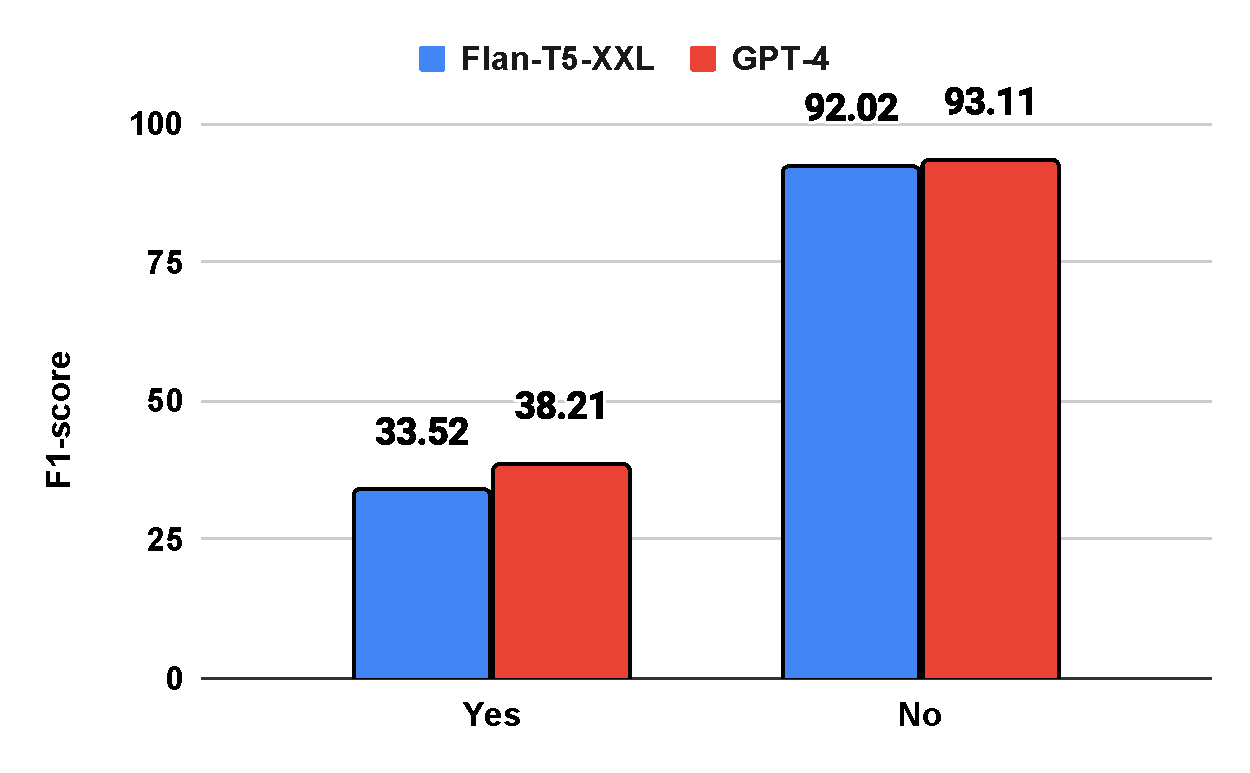
\includegraphics[width=\linewidth]{figures/gpt_4_flan_t5_xxl_social_message.pdf}
  \caption{F1-score for social message detection task class wise}
  \label{class_wise_social_message}
\end{subfigure}%
\begin{subfigure}{.50\textwidth}
  \centering
  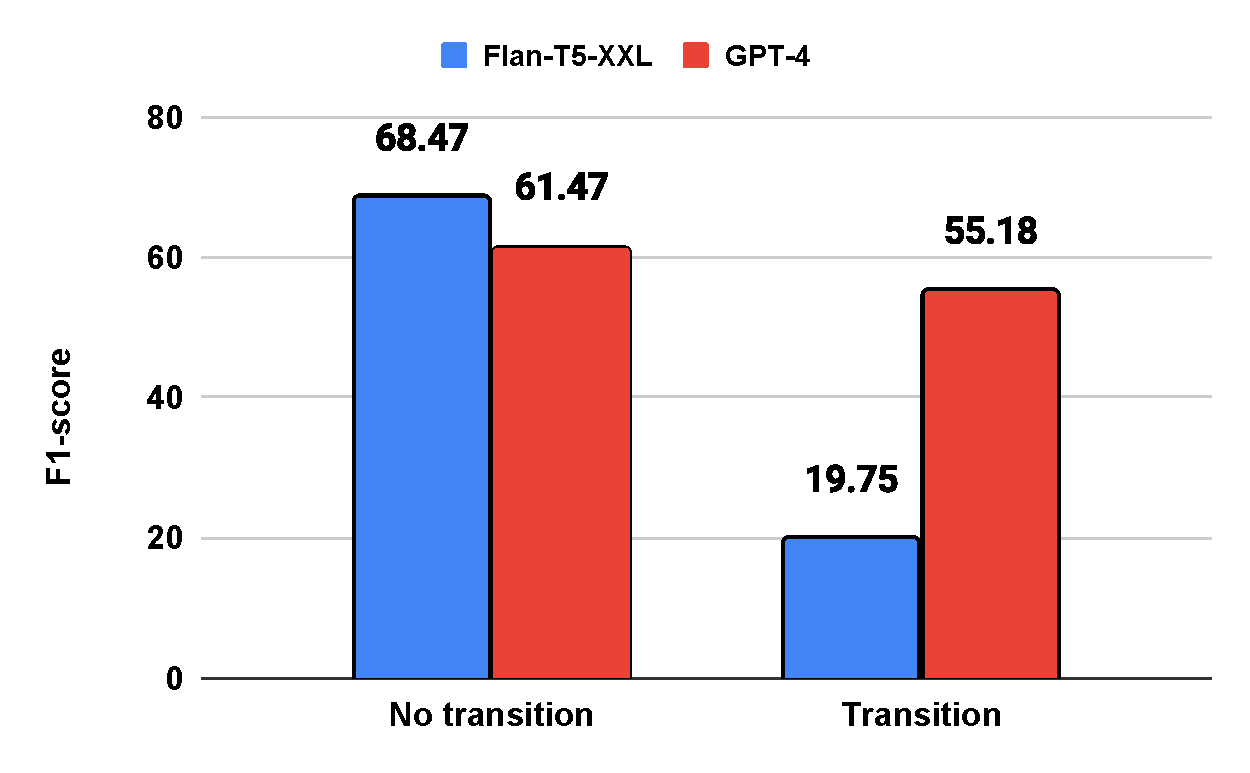
\includegraphics[width=\linewidth]{figures/gpt_4_flan_t5_xxl_transition.pdf}
  \caption{F1-score for tone transition detection task class wise}
  \label{class_wise_tone_transition}
\end{subfigure}
\caption{Comparisons between \texttt{Flan-T5-XXL} and \texttt{GPT-4} in terms of class-wise F1-score for the social message (Yes: Presence of social message, No: Absence of social message), Tone transition detection tasks.}
\label{tone_transition_social_message}
\end{figure}

\begin{figure}[h!]
    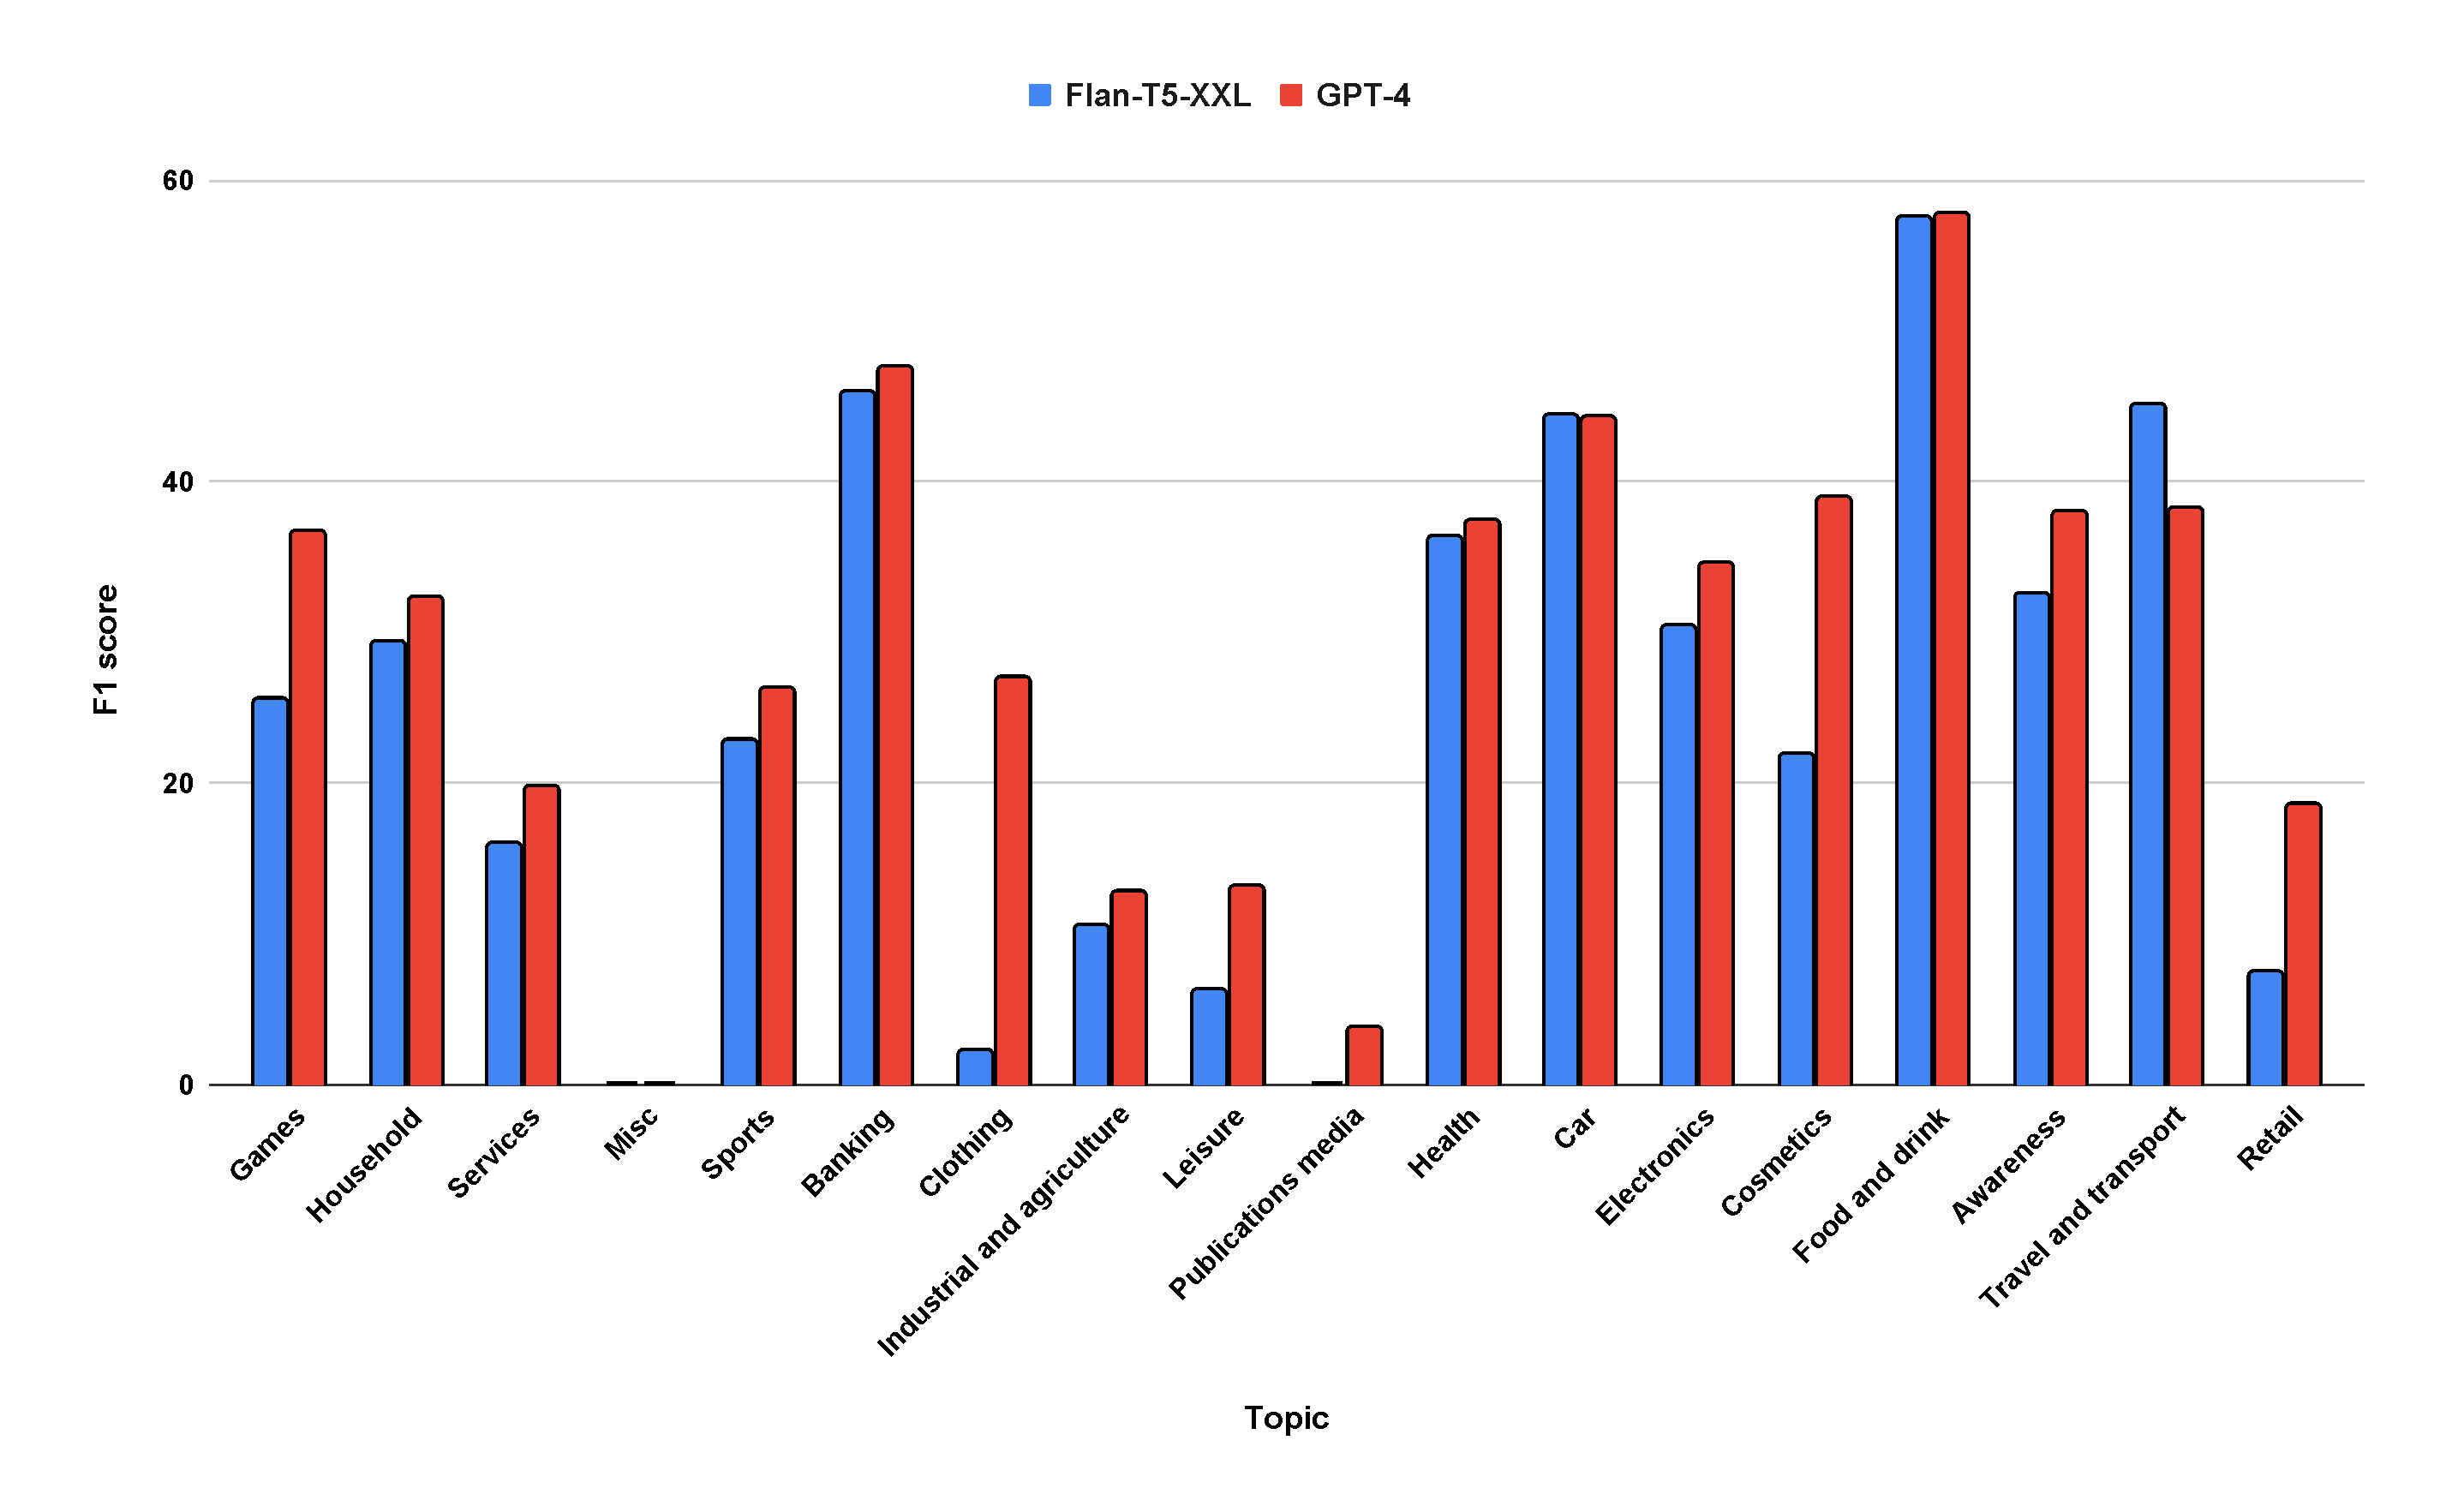
\includegraphics[width=\textwidth]{figures/gpt_4_flan_t5_xxl_topic.pdf}
    \caption{Comparisons between \texttt{Flan-T5-XXL} and \texttt{GPT-4} in terms of class-wise F1-score for the topic categorization task}
    \label{gpt_4_flan_t5_xxl_topic}
\end{figure}


\subsection{Unimodal vs Multimodal context fusion}

\begin{table}[h!]
\centering
\resizebox{\textwidth}{!}{
\begin{tabular}{|ccccccccc|}
\hline
\multicolumn{3}{|c|}{\textbf{Configurations}}                                                                               & \multicolumn{1}{c|}{\textbf{Acc}} & \multicolumn{1}{c|}{\textbf{F1}} & \multicolumn{1}{c|}{\textbf{Acc}} & \multicolumn{1}{c|}{\textbf{F1}} & \multicolumn{1}{c|}{\textbf{Acc}}   & \textbf{F1}  \\ \hline
\multicolumn{1}{|c|}{\textbf{Model}}      & \multicolumn{1}{c|}{\textbf{Features}} & \multicolumn{1}{c|}{\textbf{Modality}} & \multicolumn{2}{c|}{\textbf{Social message}}                         & \multicolumn{2}{c|}{\textbf{Tone transition}}                        & \multicolumn{2}{c|}{\textbf{Topic categorization}} \\ \hline
\multicolumn{1}{|c|}{\textbf{Random}}     & \multicolumn{1}{c|}{NA}                & \multicolumn{1}{c|}{NA}                & \multicolumn{1}{c|}{49.57±0.28}   & \multicolumn{1}{c|}{39.61±0.28}  & \multicolumn{1}{c|}{49.95±0.30}   & \multicolumn{1}{c|}{49.88±0.30}  & \multicolumn{1}{c|}{5.71±0.16}      & 4.71±0.24    \\ \hline
\multicolumn{1}{|c|}{\textbf{Majority}}   & \multicolumn{1}{c|}{NA}                & \multicolumn{1}{c|}{NA}                & \multicolumn{1}{c|}{90.96}        & \multicolumn{1}{c|}{47.63}       & \multicolumn{1}{c|}{54.11}        & \multicolumn{1}{c|}{35.11}       & \multicolumn{1}{c|}{23.04}          & 2.08         \\ \hline
\multicolumn{9}{|c|}{\textbf{Unimodal}}                                                                                                                                                                                                                                                                                        \\ \hline
\multicolumn{1}{|c|}{\textbf{LSTM}}       & \multicolumn{1}{c|}{CLIP-S}            & \multicolumn{1}{c|}{V}                 & \multicolumn{1}{c|}{90.57±0.47}   & \multicolumn{1}{c|}{68.65±1.70}  & \multicolumn{1}{c|}{61.93±0.37}   & \multicolumn{1}{c|}{61.65±0.37}  & \multicolumn{1}{c|}{52.86±0.43}     & 36.48±1.58   \\ \hline
\multicolumn{1}{|c|}{\textbf{MHA}}        & \multicolumn{1}{c|}{AST}               & \multicolumn{1}{c|}{A}                 & \multicolumn{1}{c|}{89.07±2.02}   & \multicolumn{1}{c|}{55.33±3.96}  & \multicolumn{1}{c|}{59.78±1.56}   & \multicolumn{1}{c|}{58.60±0.96}  & \multicolumn{1}{c|}{25.11±1.39}     & 15.48±1.57   \\ \hline
\multicolumn{1}{|c|}{\textbf{MHA}}        & \multicolumn{1}{c|}{CLIP-S}            & \multicolumn{1}{c|}{V}                 & \multicolumn{1}{c|}{90.41±2.24}   & \multicolumn{1}{c|}{72.28±1.66}  & \multicolumn{1}{c|}{61.74±1.07}   & \multicolumn{1}{c|}{61.48±1.11}  & \multicolumn{1}{c|}{61.30±0.89}     & 47.74±1.27   \\ \hline
\multicolumn{9}{|c|}{\textbf{Multimodal}}                                                                                                                                                                                                                                                                                      \\ \hline
\multicolumn{1}{|c|}{$\mathbf{Tx_{AT}}$}      & \multicolumn{1}{c|}{AST + BERT}        & \multicolumn{1}{c|}{A + T}             & \multicolumn{1}{c|}{90.24±0.81}   & \multicolumn{1}{c|}{64.02±0.81}  & \multicolumn{1}{c|}{62.98±0.56}   & \multicolumn{1}{c|}{62.29±0.83}  & \multicolumn{1}{c|}{42.99±0.65}     & 30.77±0.96   \\ \hline
\multicolumn{1}{|c|}{\textbf{(1) $\mathbf{Tx_{AV}}$}}  & \multicolumn{1}{c|}{CLIP-S +AST}       & \multicolumn{1}{c|}{A + V}             & \multicolumn{1}{c|}{91.62±0.58}   & \multicolumn{1}{c|}{70.05±0.67}  & \multicolumn{1}{c|}{64.01±0.54}   & \multicolumn{1}{c|}{63.72±0.66}  & \multicolumn{1}{c|}{61.62±0.46}     & 48.67±0.64   \\ \hline
\multicolumn{1}{|c|}{\textbf{(2) $\mathbf{Tx_{TV}}$}}  & \multicolumn{1}{c|}{CLIP-S +BERT}      & \multicolumn{1}{c|}{T + V}             & \multicolumn{1}{c|}{\textbf{92.23±0.57}}  & \multicolumn{1}{c|}{\textbf{74.03±1.00}}  & \multicolumn{1}{c|}{63.96±0.99}   & \multicolumn{1}{c|}{63.48±0.84}  & \multicolumn{1}{c|}{63.27±0.59}     & 50.58±1.32   \\ \hline
\multicolumn{1}{|c|}{\textbf{A-Max(1,2)}} & \multicolumn{1}{c|}{CLIP-S +BERT +AST} & \multicolumn{1}{c|}{A + V + T}          & \multicolumn{1}{c|}{92.51±0.46}   & \multicolumn{1}{c|}{73.17±1.00}  & \multicolumn{1}{c|}{\textbf{65.05±0.36}}   & \multicolumn{1}{c|}{\textbf{64.67±0.33}} & \multicolumn{1}{c|}{\textbf{65.92±0.54}}     & \textbf{54.22±1.14}  \\ \hline
\multicolumn{1}{|c|}{\textbf{D-Max(1,2)}} & \multicolumn{1}{c|}{CLIP-S +BERT +AST} & \multicolumn{1}{c|}{A + V + T}          & \multicolumn{1}{c|}{92.52±0.46}   & \multicolumn{1}{c|}{73.21±0.98}  & \multicolumn{1}{c|}{65.01±0.39}   & \multicolumn{1}{c|}{64.63±0.32}  & \multicolumn{1}{c|}{65.51±0.58}     & 53.67±1.24   \\ \hline
\end{tabular}
}
\caption{Comparative results between different unimodal and multimodal context fusion models across different tasks: Social message and Tone transition, Topic categorization. \textbf{\textit{\underline{CLIP-S}}}: Shot level features extracted using CLIP. \textbf{\textit{\underline{Modality:}}} A: Audio, V: Visual, T: Text. Results are reported as an average of 5 runs with randomly selected seeds. Best performing results are marked in bold for respective tasks.}  
\label{exptable}
\end{table}

From Table \ref{exptable}, we can see that supervised unimodal models (MHA, LSTM) show improved performance as compared to simple random and majority baselines. In terms of unimodal models, MHA model trained on shot-level visual features (denoted by CLIP-S) perform far better than audio features (AST) in social message detection (\textbf{F1: 72.28} vs \textbf{F1: 55.33}) and topic categorization tasks.
(\textbf{F1: 47.74} vs \textbf{F1: 15.48}). For the tone transition task, MHA model trained on audio features (AST) shows close performance (\textbf{F1:58.60} vs \textbf{F1: 61.48}) as compared to visual features, due to the dependence of the tone transition task on the ambient music. \\
\textbf{\underline{Multimodal models:}} For multimodal models, we observe that the fusion of text and visual modalities through a Perceiver-IO-based encoder ($\mathbf{Tx_{TV}}$) performs better (\textbf{F1:74.03}) for social message detection compared to audio-visual or audio-text fusion. This can be attributed to the presence of socially relevant descriptors in the transcripts and video shots. However, the fusion of audio with visual signals ($\mathbf{Tx_{AV}}$) improves the performance in the tone-transition detection task (\textbf{F1: 63.72}). For topic categorization, we find that the fusion of text and visual modalities ($\mathbf{Tx_{TV}}$) performs better than other paired modalities (\textbf{F1:50.58}) due to topic-specific identifiers in transcripts and shots. 
\\
 \textbf{\underline{Logit fusion:}} Our proposed approach based on logit fusion strategies: Average-Max (\textbf{A-Max}) and Dual-Max (\textbf{D-Max}) exhibits similar performance across all tasks. We obtain gain for tone-transition (\textbf{F1:64.67}) based on the \textbf{A-Max} fusion strategy of $\mathbf{Tx_{AV}}$ and $\mathbf{Tx_{TV}}$ models. In terms of class-wise metrics, \textbf{A-Max} fusion improves the transition class average F1-score to \textbf{61.28\%} as compared to $\mathbf{Tx_{AV}}$ (\textbf{60.72\%}) and $\mathbf{Tx_{TV}}$ (\textbf{60.18\%}), as seen in Fig \ref{tone_transition_social_message_multimodal} (b). However, we observe from Fig \ref{tone_transition_social_message_multimodal} (a), that both average-Max (\textbf{A-Max}) and dual-Max (\textbf{D-Max}) fusion strategies do not help for social message detection (i.e., \textbf{Yes} class).
 In the case of topic categorization, logit fusion through \textbf{A-Max} of $\mathbf{Tx_{AV}}$ and $\mathbf{Tx_{TV}}$ models results in the best performance (\textbf{F1: 54.22}). Further, \textbf{A-Max} fusion results in improvements over $\mathbf{Tx_{AV}}$ and $\mathbf{Tx_{TV}}$ across 15 topic categories (out of 18), with noticeable gains in the minority categories i.e., Retail ($\sim${\textbf{6.2\%}}), Industrial \& Agriculture ($\sim$\textbf{5\%}), Household ($\sim$\textbf{7\%}). Similar trends can be observed for \textbf{D-Max} fusion, with improvements obtained across 14 topic categories (out of 18). The detailed comparisons between $\mathbf{Tx_{AV}}$,  $\mathbf{Tx_{TV}}$, \textbf{A-Max} and \textbf{D-Max} can be found in Fig \ref{topic_multimodal}.


 \begin{figure}[h!]
\begin{subfigure}{.50\textwidth}
  \centering
  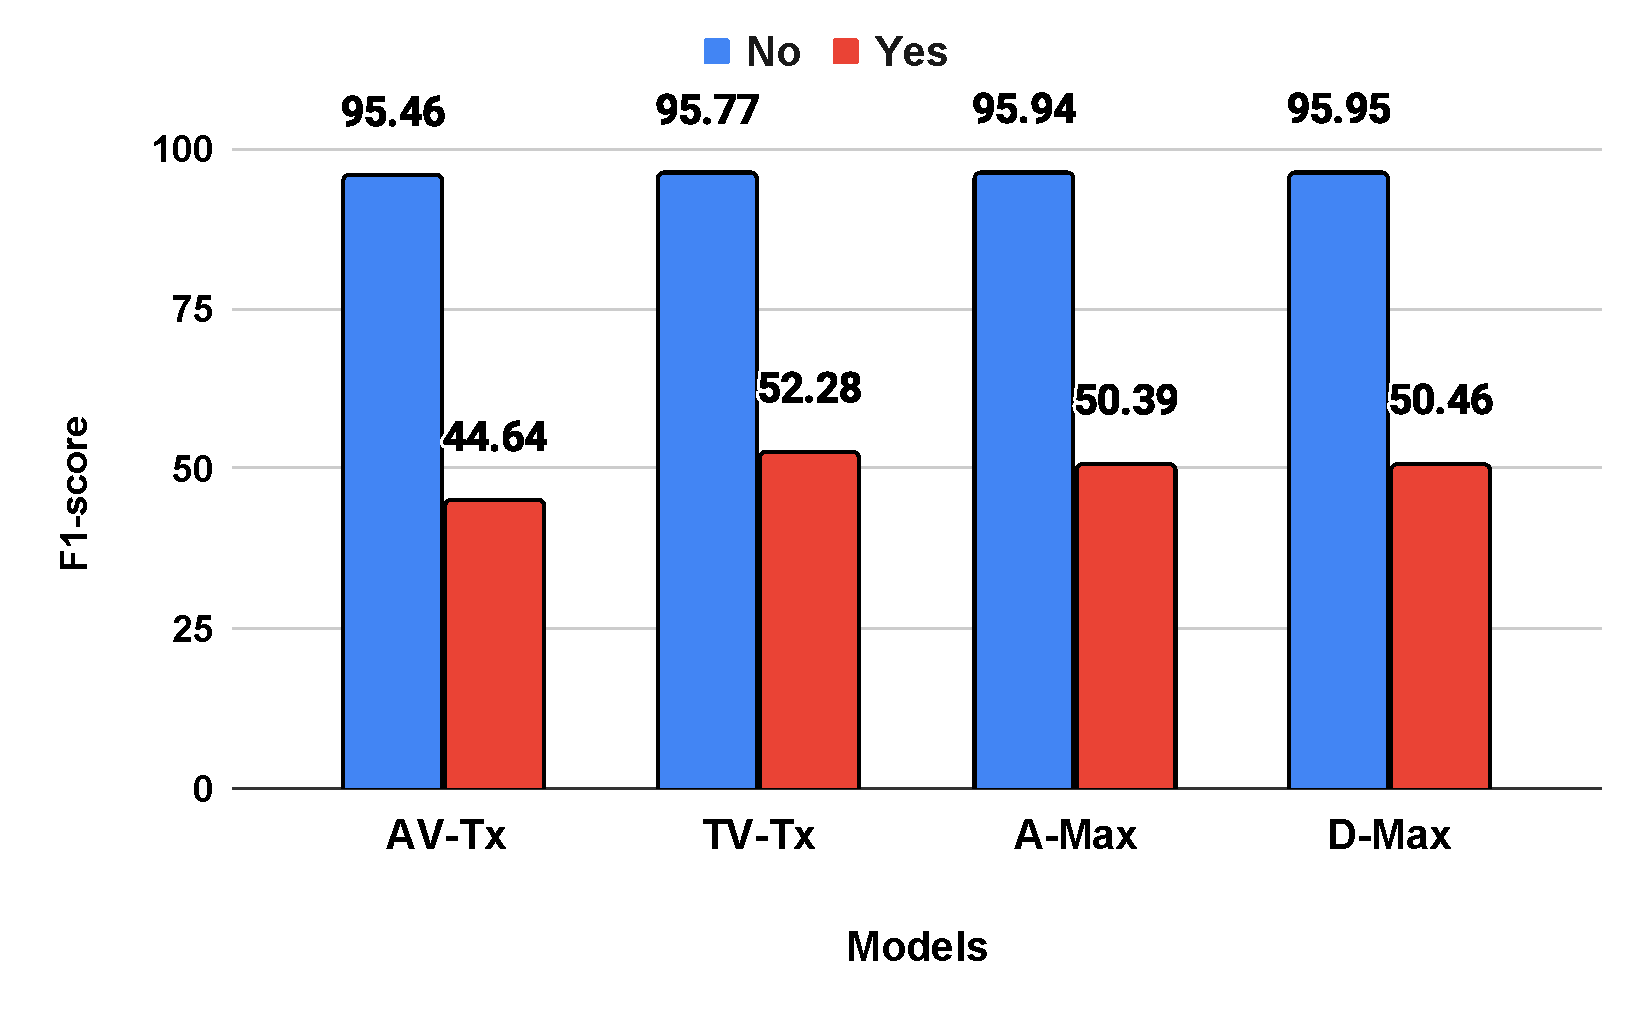
\includegraphics[width=\linewidth]{figures/multimodal_baselines_f1_score_social_message.pdf}
  \caption{F1-score for social message detection task class-wise}
  \label{class_wise_social_message_multimodal}
\end{subfigure}%
\begin{subfigure}{.50\textwidth}
  \centering
  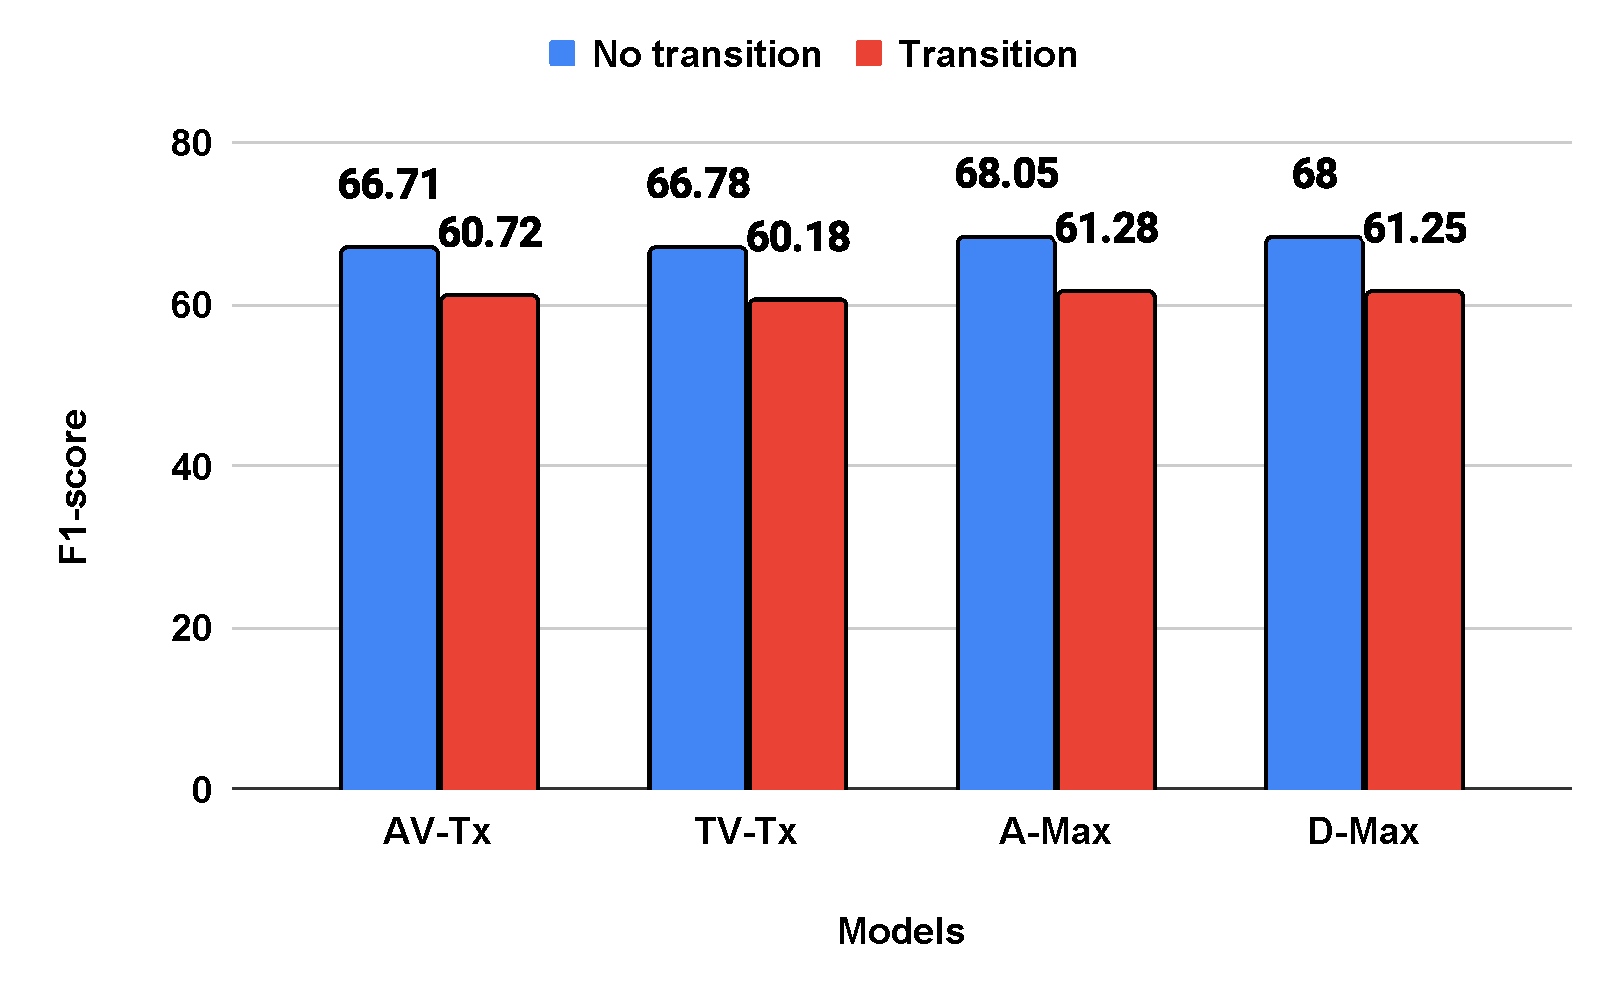
\includegraphics[width=\linewidth]{figures/multimodal_baselines_f1_score_transition.pdf}
  \caption{F1-score for tone transition detection task class-wise}
  \label{class_wise_tone_transition_multimodal}
\end{subfigure}
\caption{Comparisons between $\mathbf{Tx_{AV}}$(\texttt{AV-Tx}), $\mathbf{Tx_{TV}}$(\texttt{TV-Tx}), \texttt{A-Max}, \texttt{D-Max} in terms of class-wise F1-score for the social message (Yes: Presence of social message, No: Absence of social message), Tone transition detection tasks. Average of 5 runs considered for the F1-score.}
\label{tone_transition_social_message_multimodal}
\end{figure}

 \begin{figure*}[h!]
    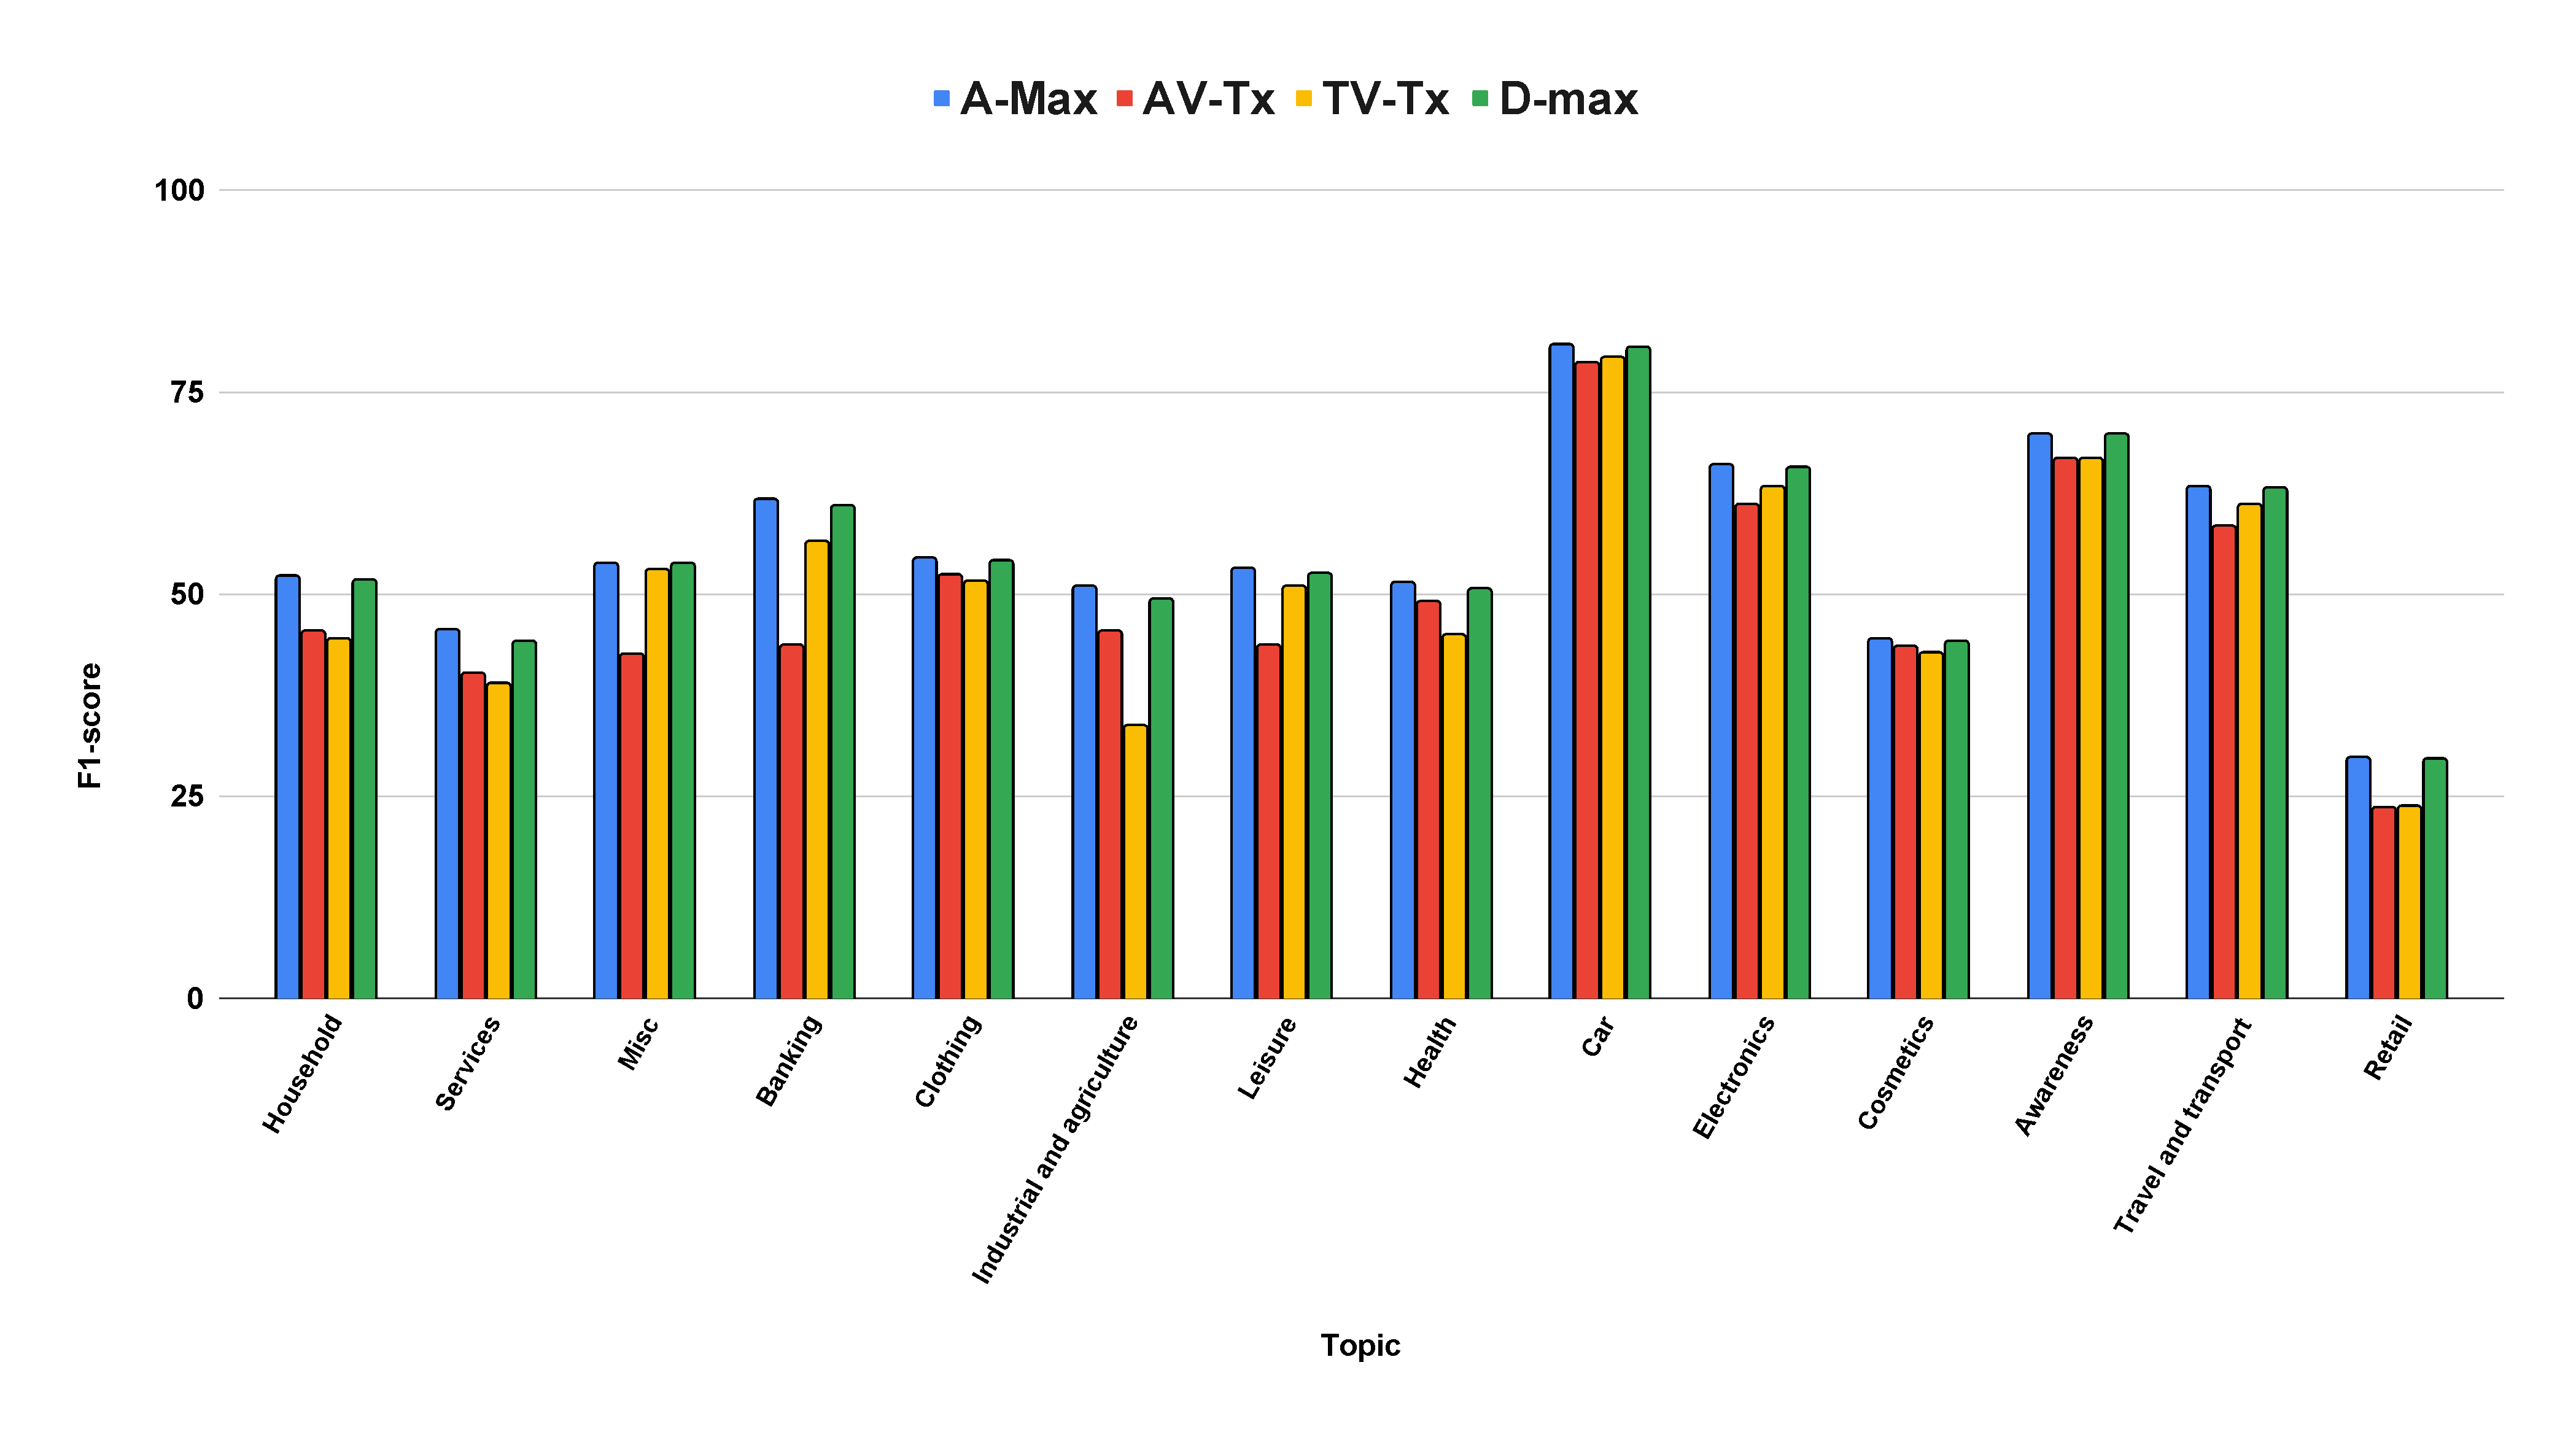
\includegraphics[width=\textwidth]{figures/multimodal_baselines_f1_score_topic.pdf}
    \caption{Comparisons between $\mathbf{Tx_{AV}}$ (\texttt{AV-Tx}), $\mathbf{Tx_{TV}}$(\texttt{TV-Tx}), \textbf{A-Max}, \textbf{D-Max} in terms of class-wise F1-score for the topic categorization task. Average of 5 runs is considered for the F1-score.}
    \label{topic_multimodal}
\end{figure*}

\section{Conclusions}

We introduce a benchmark called MM-AU for a macro-level understanding of advertisement videos. Further, we consider the narrative-driven tasks of topic categorization, tone transition, and social message detection. 
The major takeaways from this work are as follows:

\begin{itemize}

\item \textbf{Context-fusion:} Temporal and foreground context fusion through multiple modalities enable macro-level understanding of advertisement videos.

\item \textbf{Narrative-driven understanding:} The proposed tasks can be further extended to include explicit modeling of context-based narrative transitions.

\item \textbf{Importance of modalities:} As seen from the individual task-specific results, not all modalities contain useful signals. For a given macro-level task, there is a need to find the optimal fusion of context streams that can depend on a subset of input modalities.

\end{itemize}



